\chapter{BDT Input Variables}\label{app:bdt}
\section{List of all potential Input Features}\label{appsec:bdtFeatures}
Following the application of the event selection criteria, as described in Chapter~\ref{chapter:tzq-search}, a large number of input variables which were considered for use in the boosted decision trees used were constructed from the selected reconstructed physics objects.

The complete list of variables and their descriptions are listed in table~\ref{tab:allBdtVariables}.

\begin{table}[htbp]
\topcaption {The list of the names and descriptions of all of variables considered by recursive feature elimination to be used as input to the BDT to discriminate between potential tZq signal events and the dominant backgrounds.
}
\label{tab:allBdtVariables}
  \centering
% This increases column spacing.
\resizebox{\textwidth}{!}{
% This right-aligns numbers in column, but centers them under column title.
\begin{tabular}{cc}
   \hline
   \textbf{Variable} & \textbf{Description} \\
   \hline
    wQuark1Pt & Leading W boson candidate jet \pt \\
    wQuark1Eta & Leading W boson candidate jet $\eta$ \\
    wQuark1Phi &  Leading W boson candidate jet $\phi$ \\
    wQuark2Pt & Subleading W boson candidate jet \pt \\
    wQuark2Eta & Subleading W boson candidate jet $\eta$ \\
    wQuark2Phi & Subleading W boson candidate jet $\phi$  \\
    wPairMass & Reconstructed W boson mass  \\
    wPairPt & Reconstructed W boson \pt  \\
    wPairEta & Reconstructed W boson $\eta$  \\
    wPairPhi & Reconstructed W boson $\phi$  \\
    mTW & W boson transverse mass  \\
    met & Missing transverse energy   \\
    nJets & Number of jets  \\
    j1j2delR & $\Delta R$ between the leading and subleading jets \\
    j1j2delPhi & $\Delta \phi$ between the leading and subleading jets \\
    leadJetPt & Leading jet \pt \\
    leadJetPhi & Leading jet $\phi$  \\
    leadJetEta & Leading jet $\eta$  \\
    leadJetbTag & Leading jet b-tag output discriminant  \\
    secJetPt & Subleading jet \pt \\
    secJetPhi & Subleading jet $\phi$  \\
    secJetEta & Subleading jet $\eta$ \\
    secJetbTag & Subleading jet b-tag output discriminant  \\
   \hline
 \end{tabular}}
\end{table}

\begin{table}[htbp]
\label{tab:allBdtVariables2}
  \centering
% This increases column spacing.
\resizebox{\textwidth}{!}{
% This right-aligns numbers in column, but centers them under column title.
\begin{tabular}{cc}
   \hline
   \textbf{Variable} & \textbf{Description} \\
   \hline
    thirdJetPt & Third jet \pt \\
    thirdJetPhi & Third jet $\phi$  \\
    thirdJetEta & Third jet $\eta$ \\
    thirdJetbTag & Third jet b-tag output discriminant  \\
    fourthJetPt & Fourth jet \pt \\
    fourthJetPhi & Fourth jet $\phi$  \\
    fourthJetEta & Fourth jet $\eta$ \\
    fourthJetbTag & Fourth jet b-tag output discriminant  \\
    nBjets & Number of b-tagged jets \\
    bTagDisc & Leading b-tagged jet b-tag output discriminant \\
    lep1Pt & Leading lepton \pt \\
    lep1Eta & Leading lepton $\eta$ \\
    lep1Phi & Leading lepton $\phi$ \\
    lep1RelIso & Leading lepton $I^{rel}$ \\
    lep1D0 & Leading lepton $d_{0}$ \\
    lep2Pt & Subleading lepton \pt \\
    lep2Eta & Subleading lepton $\eta$ \\
    lep2Phi & Subleading lepton $\phi$ \\
    lep2RelIso & Subleading lepton $I^{rel}$ \\
    lep2D0 & Subleading lepton $d_{0}$ \\
    zMass & Z boson mass  \\
    zPt & Reconstructed Z boson \pt \\
    zEta & Reconstructed Z boson $\eta$ \\
    zPhi & Reconstructed Z boson $\phi$ \\
    topMass & Reconstructed top quark mass \\
    topPt & Reconstructed top quark \pt \\
    topEta & Reconstructed top quark $\eta$ \\
    topPhi & Reconstructed top quark $\phi$ \\
    w1w2delR & $\Delta R$ between the W boson candidate's jets \\
    w1w2delPhi & $\Delta \phi$ between the W boson candidate's jets \\
    zLepdelR & $\Delta R$ between the Z boson candidate leptons \\
    zLepdelPhi & $\Delta \phi$ between the Z boson candidates leptons \\
    zl1Quark1DelR & $\Delta R$ between the leading lepton and W boson candidate's leading jet \\
    zl1Quark1DelPhi & $\Delta \phi$ between the leading lepton and W boson candidate's leading jet \\
    zl1Quark2DelR & $\Delta R$ between the leading lepton and W boson candidate's subleading jet \\
    zl1Quark2DelPhi & $\Delta \phi$ between the leading lepton and W boson candidate's subleading jet \\
    zl2Quark1DelR & $\Delta R$ between the subleading lepton and W boson candidate's leading jet \\
    zl2Quark1DelPhi & $\Delta \phi$ between the subleading lepton and W boson candidate's leading jet \\
    zl2Quark2DelR & $\Delta R$ between the subleading lepton and W boson candidate's subleading jet \\
    zl2Quark2DelPhi & $\Delta \phi$ between the subleading lepton and W boson candidate's subleading jet \\
    zlb1DelR & $\Delta R$ between the leading lepton and leading b-tagged jet \\
    zlb1DelPhi & $\Delta \phi$ between the leading lepton and leading b-tagged jet \\
    zlb2DelR & $\Delta R$ between the subleading lepton and leading b-tagged jet\\
    zlb2DelPhi & $\Delta \phi$ between the subleading lepton and leading b-tagged jet \\
    lepHt & ${\ensuremath{H_{\mathrm{T}}}}$ of the Z boson candidate's leptons \\
    wQuarkHt & ${\ensuremath{H_{\mathrm{T}}}}$ of the W boson candidate's jets \\
   \hline
 \end{tabular}}
\end{table}

\begin{table}[htbp]
\label{tab:allBdtVariables3}
  \centering
% This increases column spacing.
\resizebox{\textwidth}{!}{
% This right-aligns numbers in column, but centers them under column title.
\begin{tabular}{cc}
   \hline
   \textbf{Variable} & \textbf{Description} \\
   \hline
    totPtVec & \pt of the system \\
    totEta & $\eta$ of the system \\
    totPhi & $\phi$ of the system \\
    totVecM & Invariant mass of the system \\
    totPt2Jet & Square of the sum of the two leading jets' \pT \\
    totJetPt & Sum of all the jets' \pT  \\
    wZdelR & $\Delta R$ between the W and Z boson candidates \\
    wZdelPhi & $\Delta \phi$ between the W and Z bosons candidates \\
    zQuark1DelR & $\Delta R$ between the Z boson candidate and W boson candidate's leading jet \\
    zQuark1DelPhi & $\Delta \phi$ between the Z boson candidate and W boson candidate's leading jet \\
    zQuark2DelR & $\Delta R$ between the Z boson candidate and W boson candidate's subleading jet \\
    zQuark2DelPhi & $\Delta \phi$ between the Z boson candidate and W boson candidate's subleading jet \\
    zTopDelR & $\Delta R$ between the Z boson and top quark candidates \\
    zTopDelPhi & $\Delta \phi$ between the Z boson and top quark candidates\\
    zl1TopDelR & $\Delta R$ between the leading lepton and top quark candidates \\
    zl1TopDelPhi & $\Delta \phi$ between the leading lepton and top quark candidates \\
    zl2TopDelR & $\Delta R$ between the subleading lepton and top quark candidate \\
    zl2TopDelPhi & $\Delta \phi$ between the subleading lepton and top quark candidate \\
    wTopDelR & $\Delta R$ between the W boson and top quark candidates \\
    wTopDelPhi & $\Delta \phi$ between the W boson and top quark candidates \\
    w1TopDelR & $\Delta R$ between the W boson candidates's leading jet and the top quark candidate\\
    w1TopDelPhi & $\Delta \phi$ between the W boson candidates's leading jet and the top quark candidate \\
    w2TopDelR & $\Delta R$ between the W boson candidates's subleading jet and the top quark candidate \\
    w2TopDelPhi & $\Delta \phi$ between the W boson candidates's subleading jet and the top quark candidate \\
    zjminR & Minimum $\Delta R$ between the Z boson candidate and any jet  \\
    minZJetPhi & Minimum $\phi R$ between the Z boson candidate and any jet \\
    totHt & Total ${\ensuremath{H_{\mathrm{T}}}}$ of the system \\
    jetHt & ${\ensuremath{H_{\mathrm{T}}}}$ of all the jets in an event \\
    jetMass & Invariant mass of all the jets in an event \\
    jetPt & \pT of all the jets in an event \\
    jetEta & $\eta$ of all the jets in an event \\
    jetPhi & $\phi$ of all the jets in an event \\
    jetMass3 & Invariant mass of the leading three jets in an event\\
    totHtOverPt & Total ${\ensuremath{H_{\mathrm{T}}}}$ divided by the system's \pT \\
   \hline
 \end{tabular}}
\end{table}

\section{List of all potential Input Features}\label{appsec:bdtInputComparisons}
The following section contains the full set of comparison plots between data and simulation for the chosen BDT input variables listed in table~\ref{selectedBdtVariables} in Section~\ref{subsec:bdtOpt}.

\begin{figure}[htb]
\centering
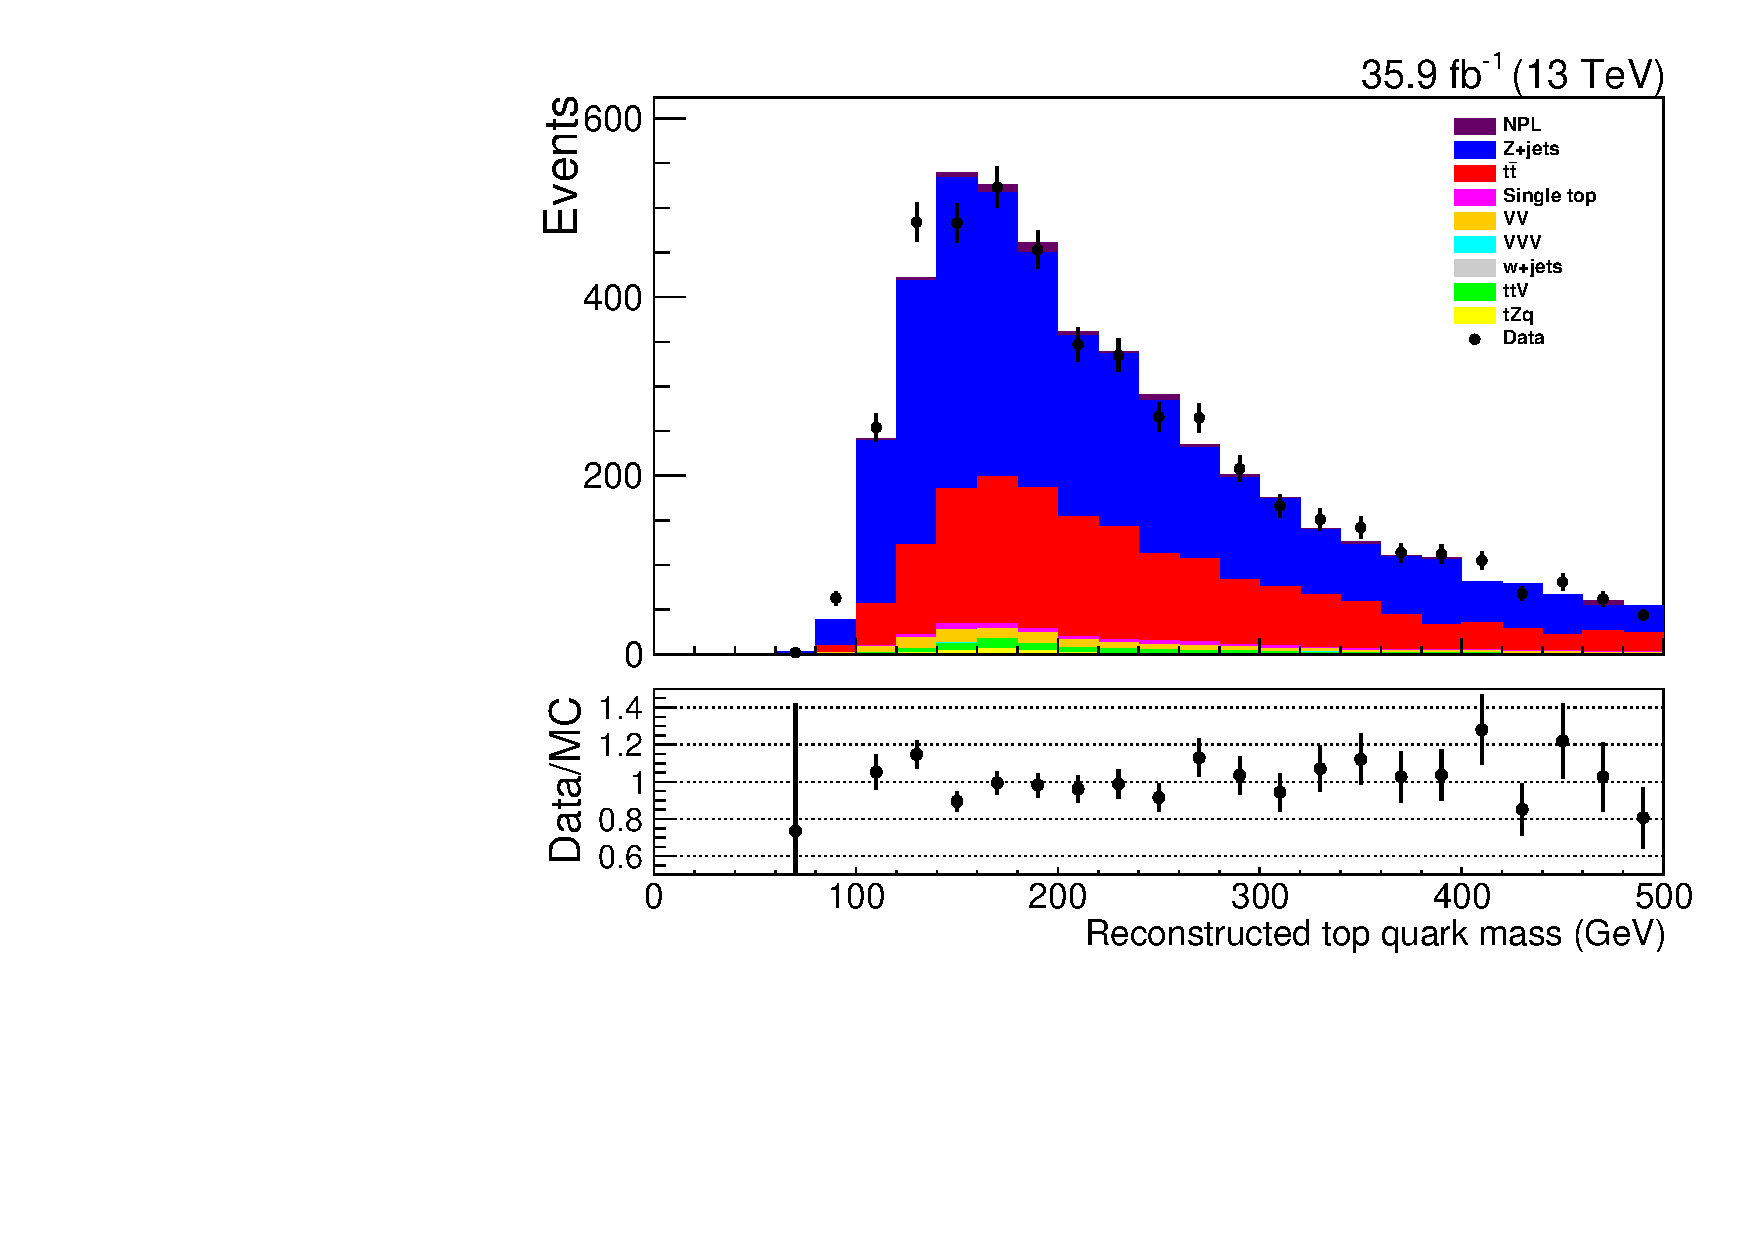
\includegraphics[width=0.47\textwidth]{figs/background-estimation/plots/unblinded/prompt_ee_ttbarInc/topMass_NPL_ee_wMass_ee.pdf}
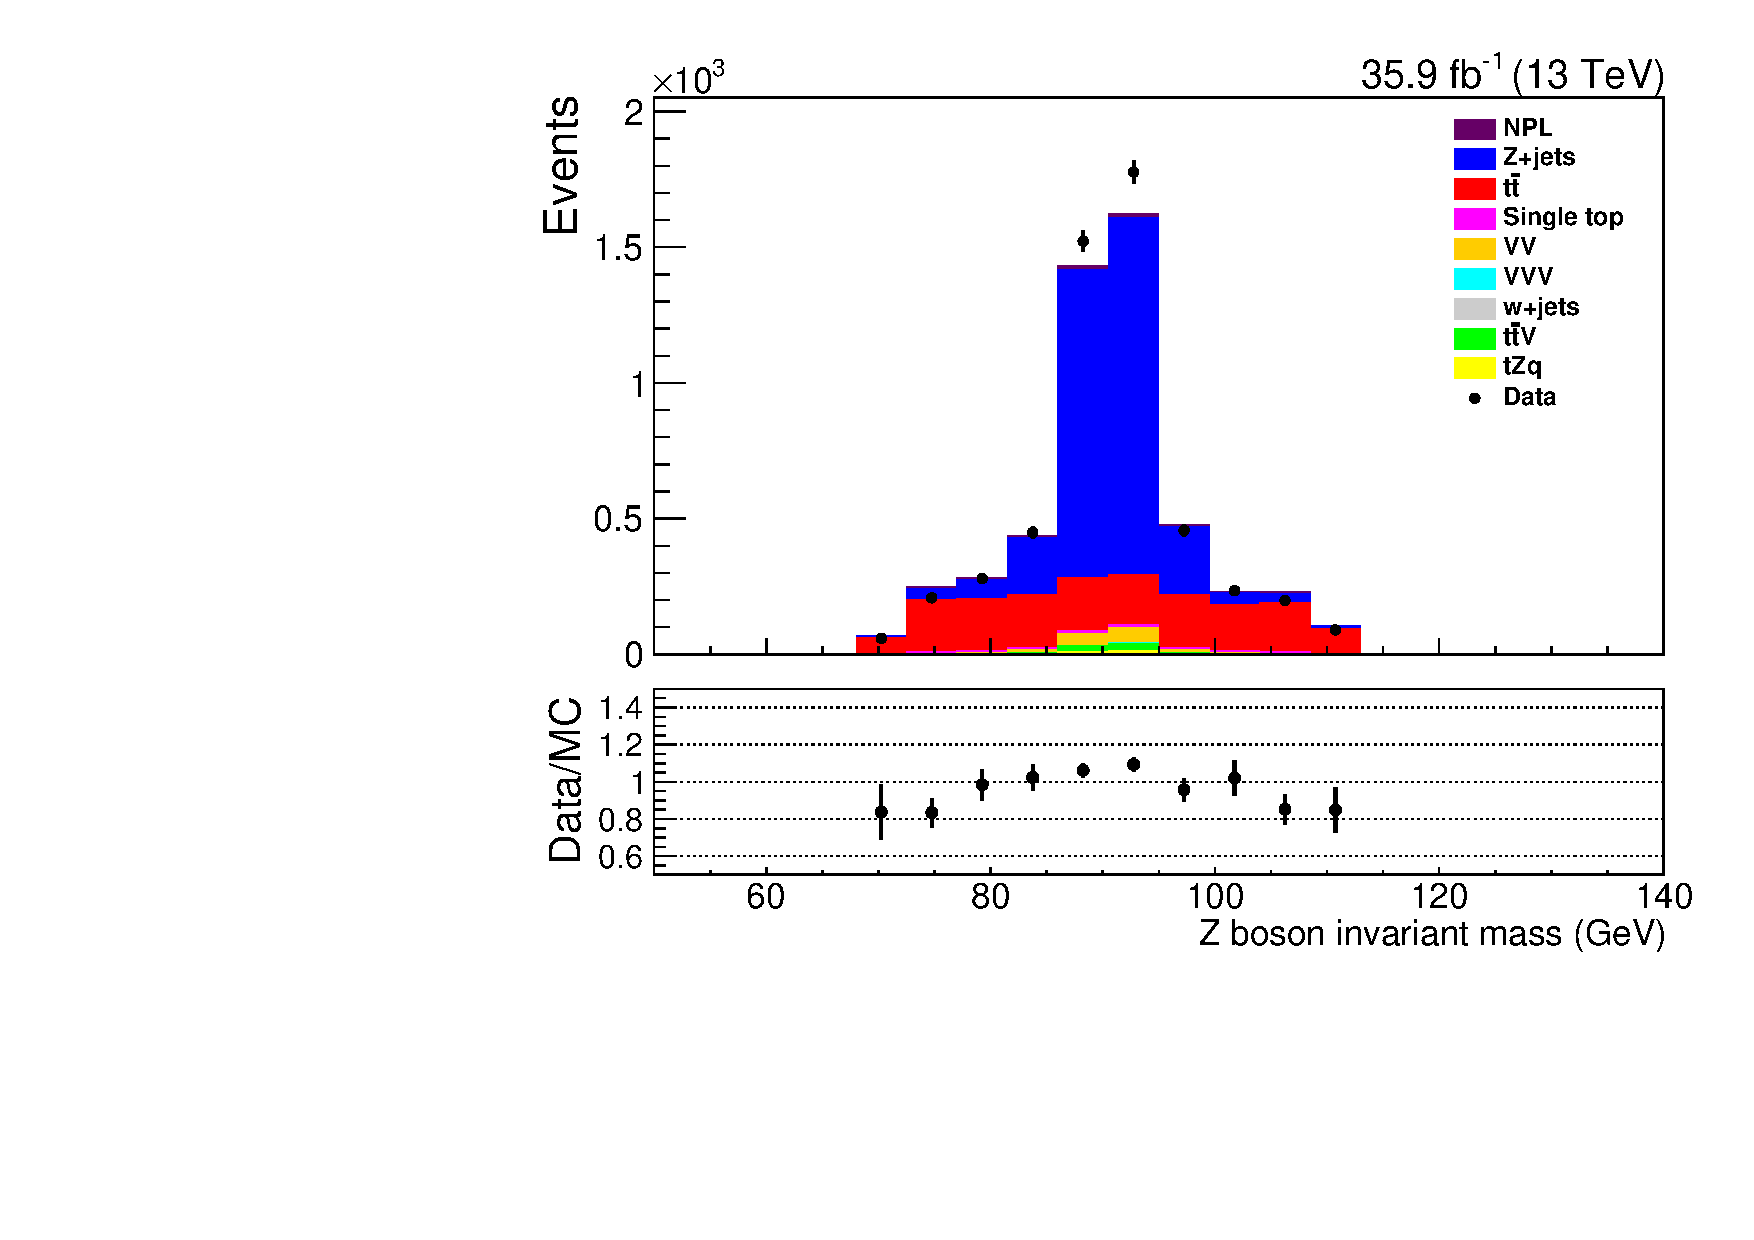
\includegraphics[width=0.47\textwidth]{figs/background-estimation/plots/unblinded/prompt_ee_ttbarInc/zPairMass_NPL_ee_wMass_ee.pdf}
\\
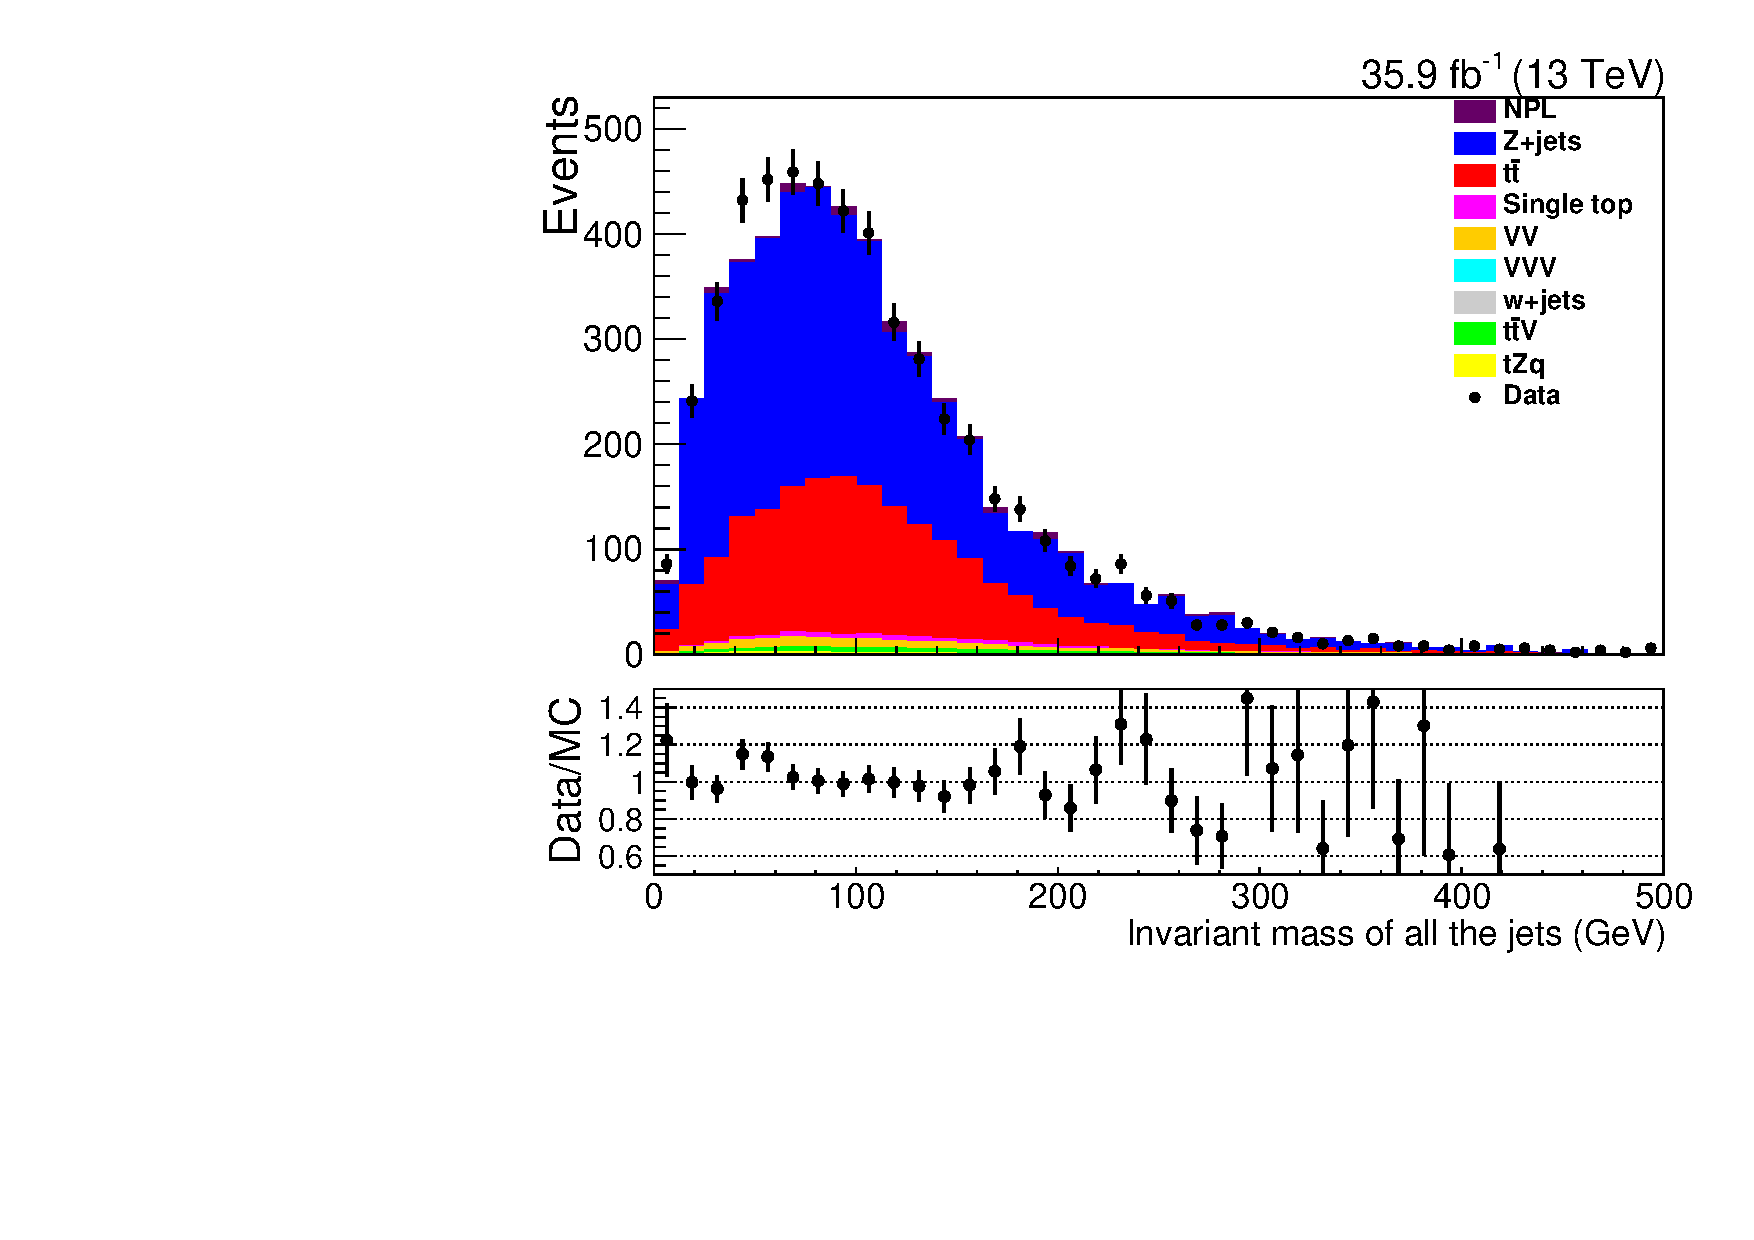
\includegraphics[width=0.47\textwidth]{figs/background-estimation/plots/unblinded/prompt_ee_ttbarInc/totalJetMass_NPL_ee_wMass_ee.pdf}
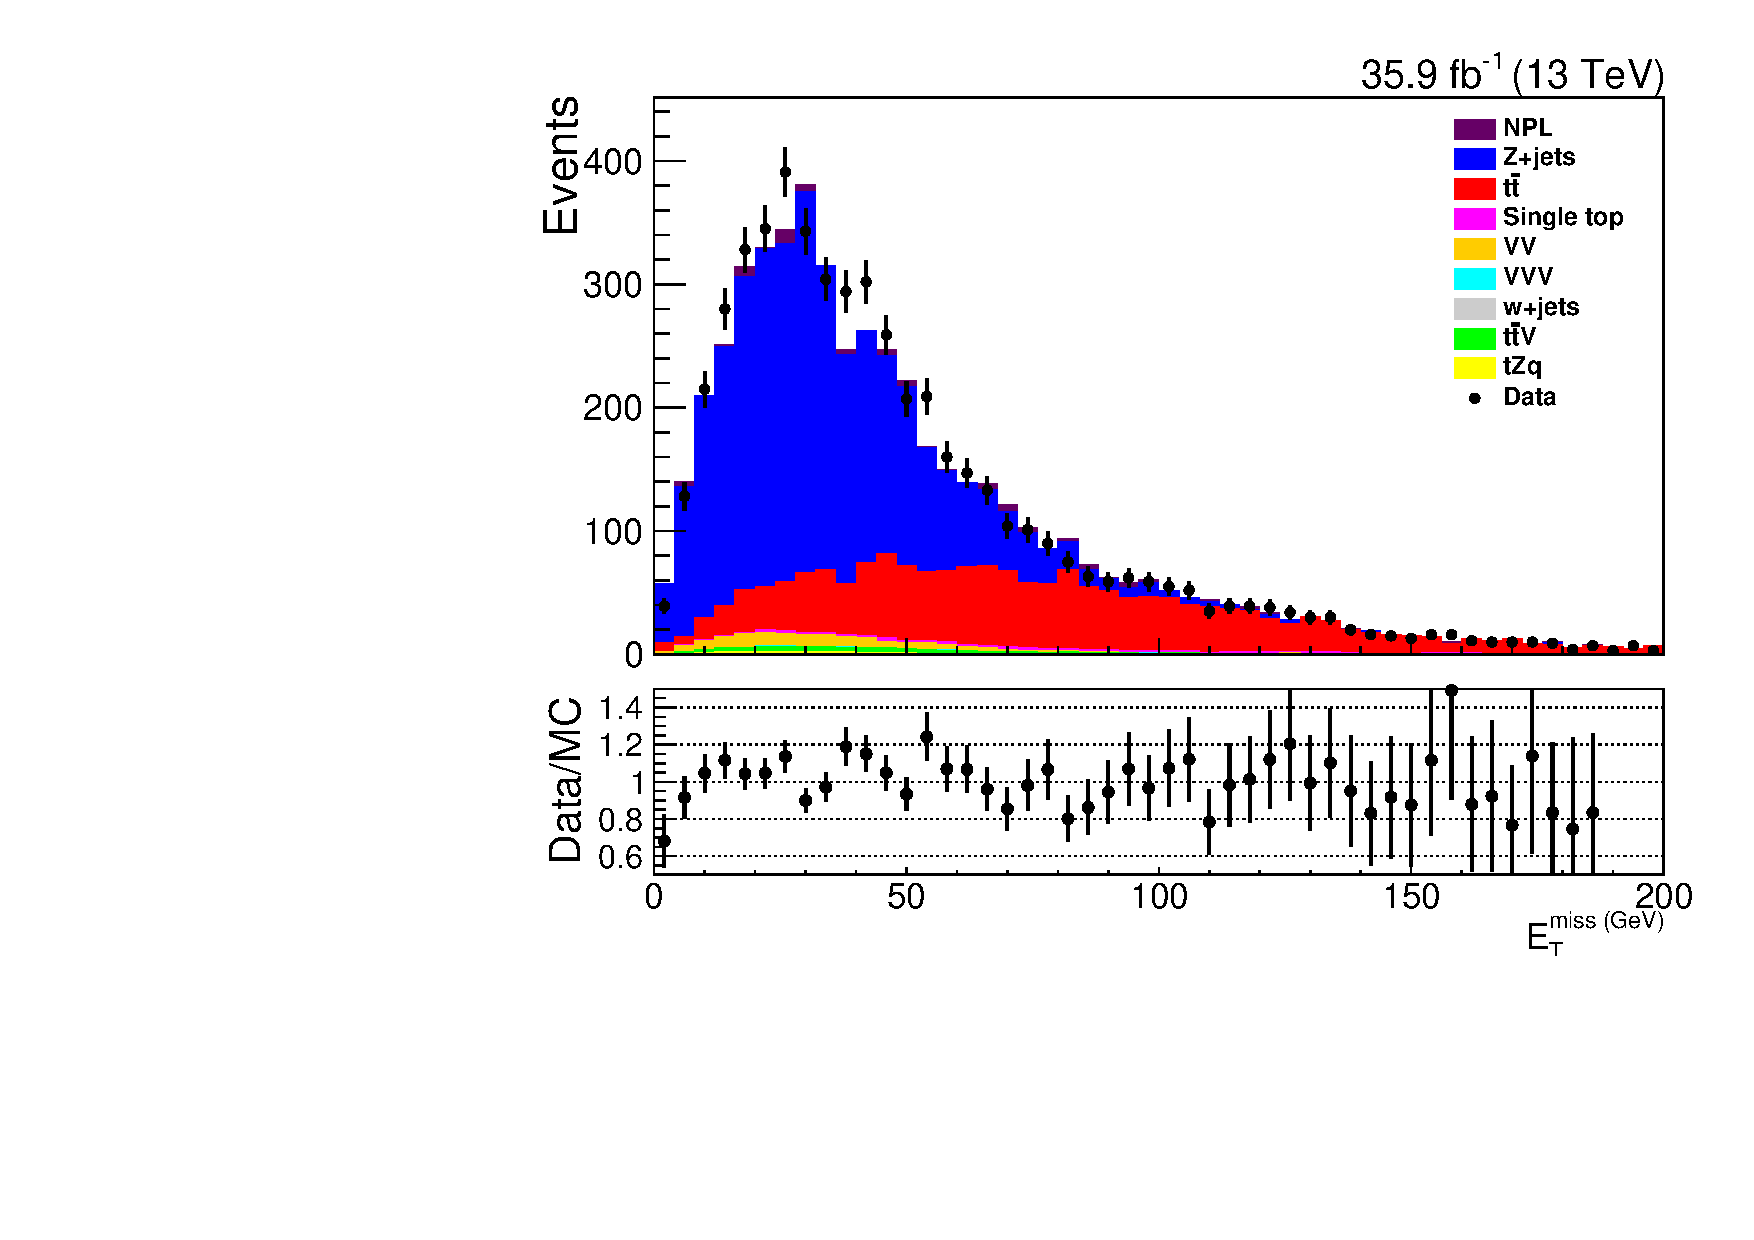
\includegraphics[width=0.47\textwidth]{figs/background-estimation/plots/unblinded/prompt_ee_ttbarInc/met_NPL_ee_wMass_ee.pdf}
\caption{
Reconstructed top mass, Z boson mass, total jet mass, and \MET distributions for the $ee$ channel comparing the agreement between data and simulation for the variables used as input variables in the BDT training.}
\label{fig:appInputFeaturesDataSimAgreement0}
\end{figure}

\begin{figure}[htb]
\centering
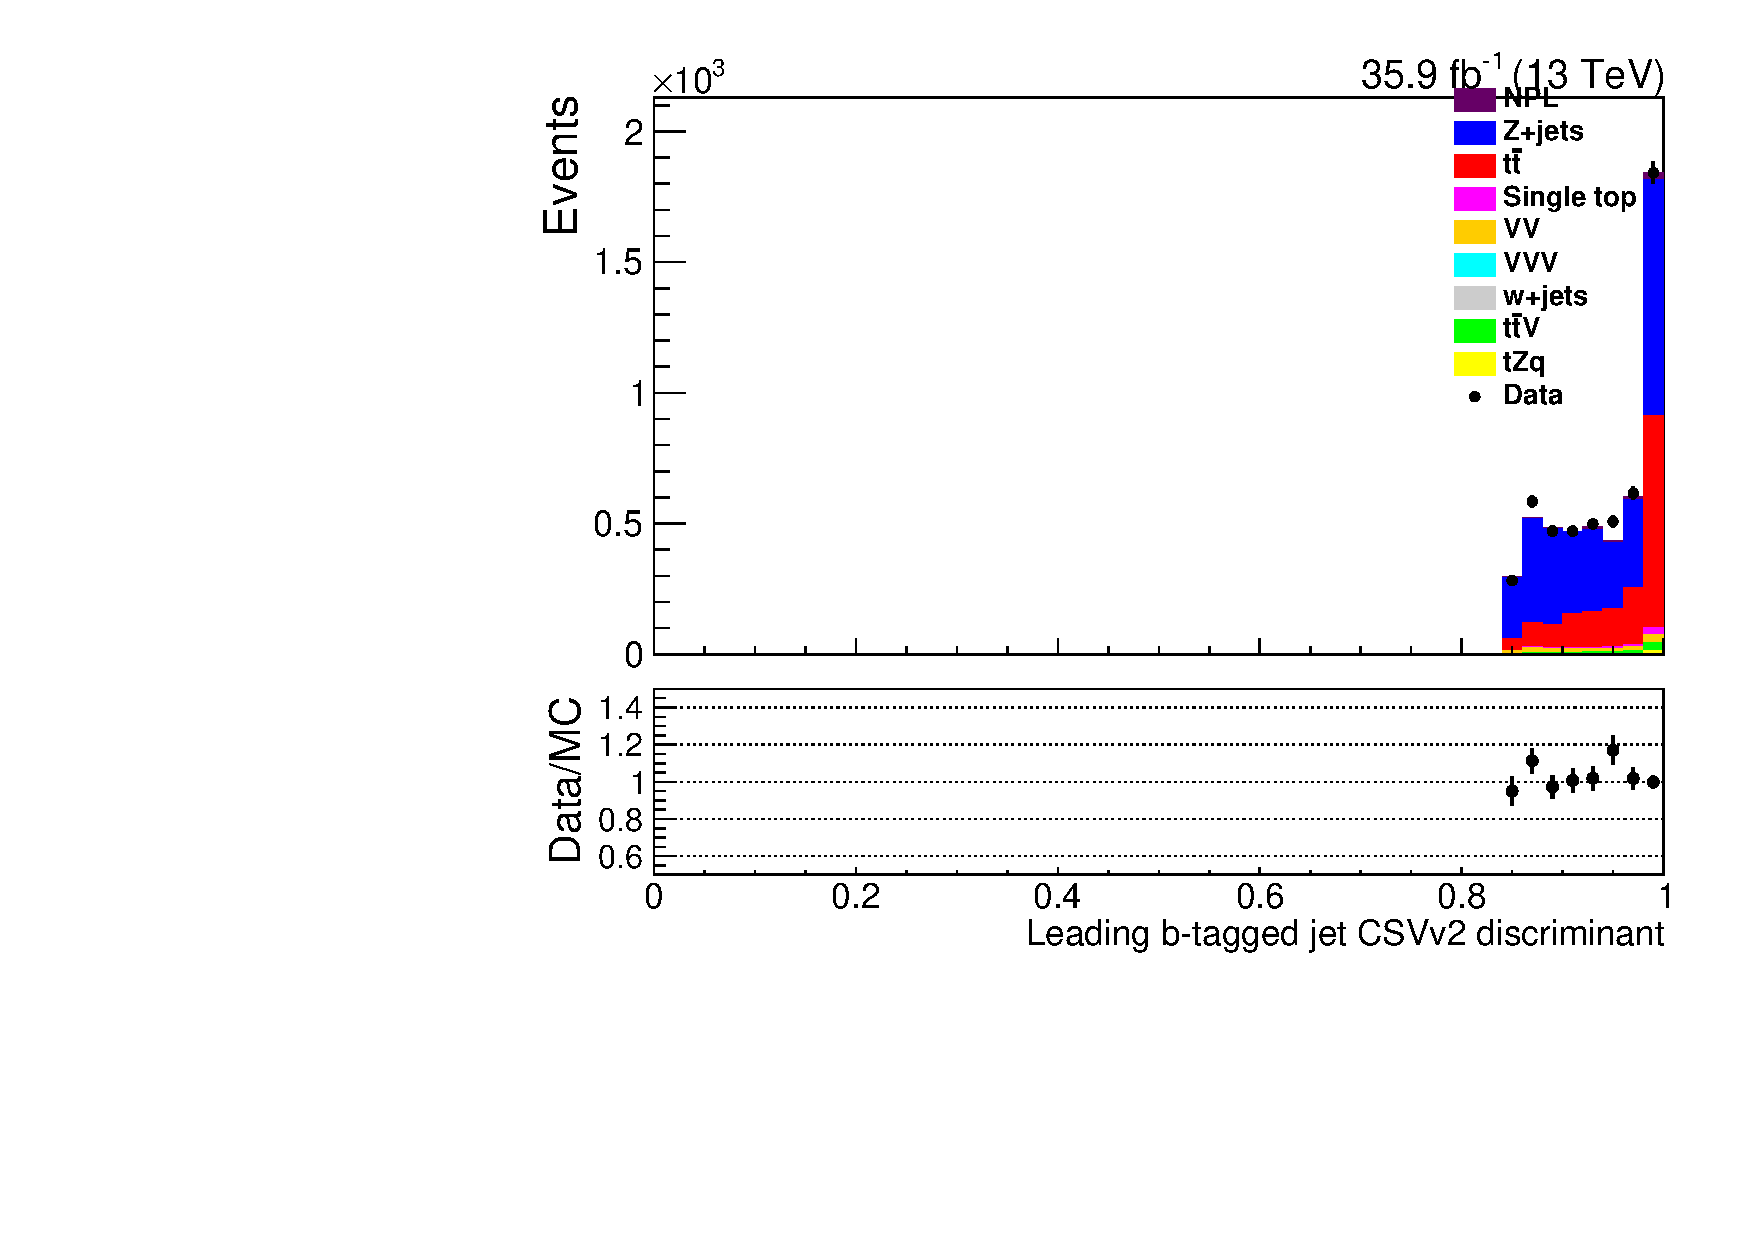
\includegraphics[width=0.47\textwidth]{figs/background-estimation/plots/unblinded/prompt_ee_ttbarInc/bTagDisc_NPL_ee_wMass_ee.pdf}
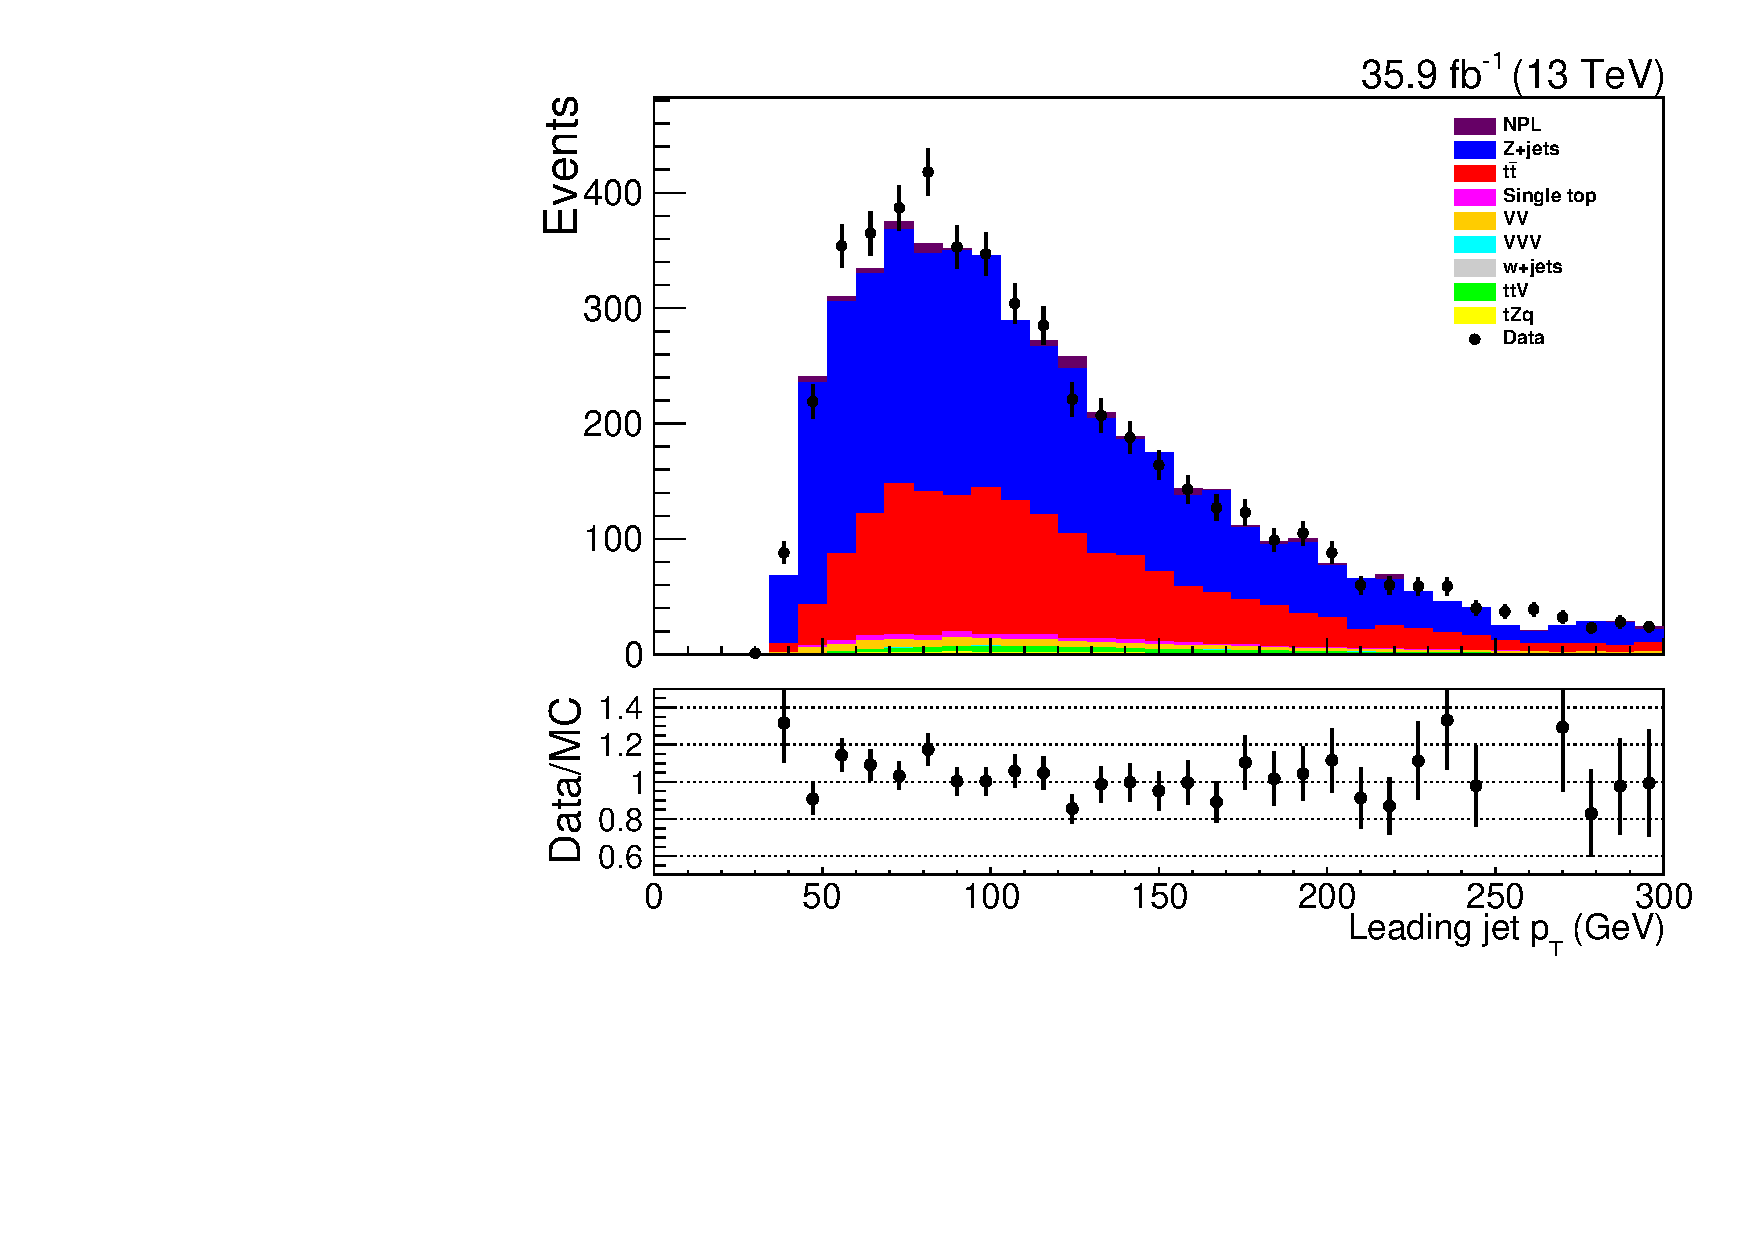
\includegraphics[width=0.47\textwidth]{figs/background-estimation/plots/unblinded/prompt_ee_ttbarInc/leadingJetPt_NPL_ee_wMass_ee.pdf}
\\
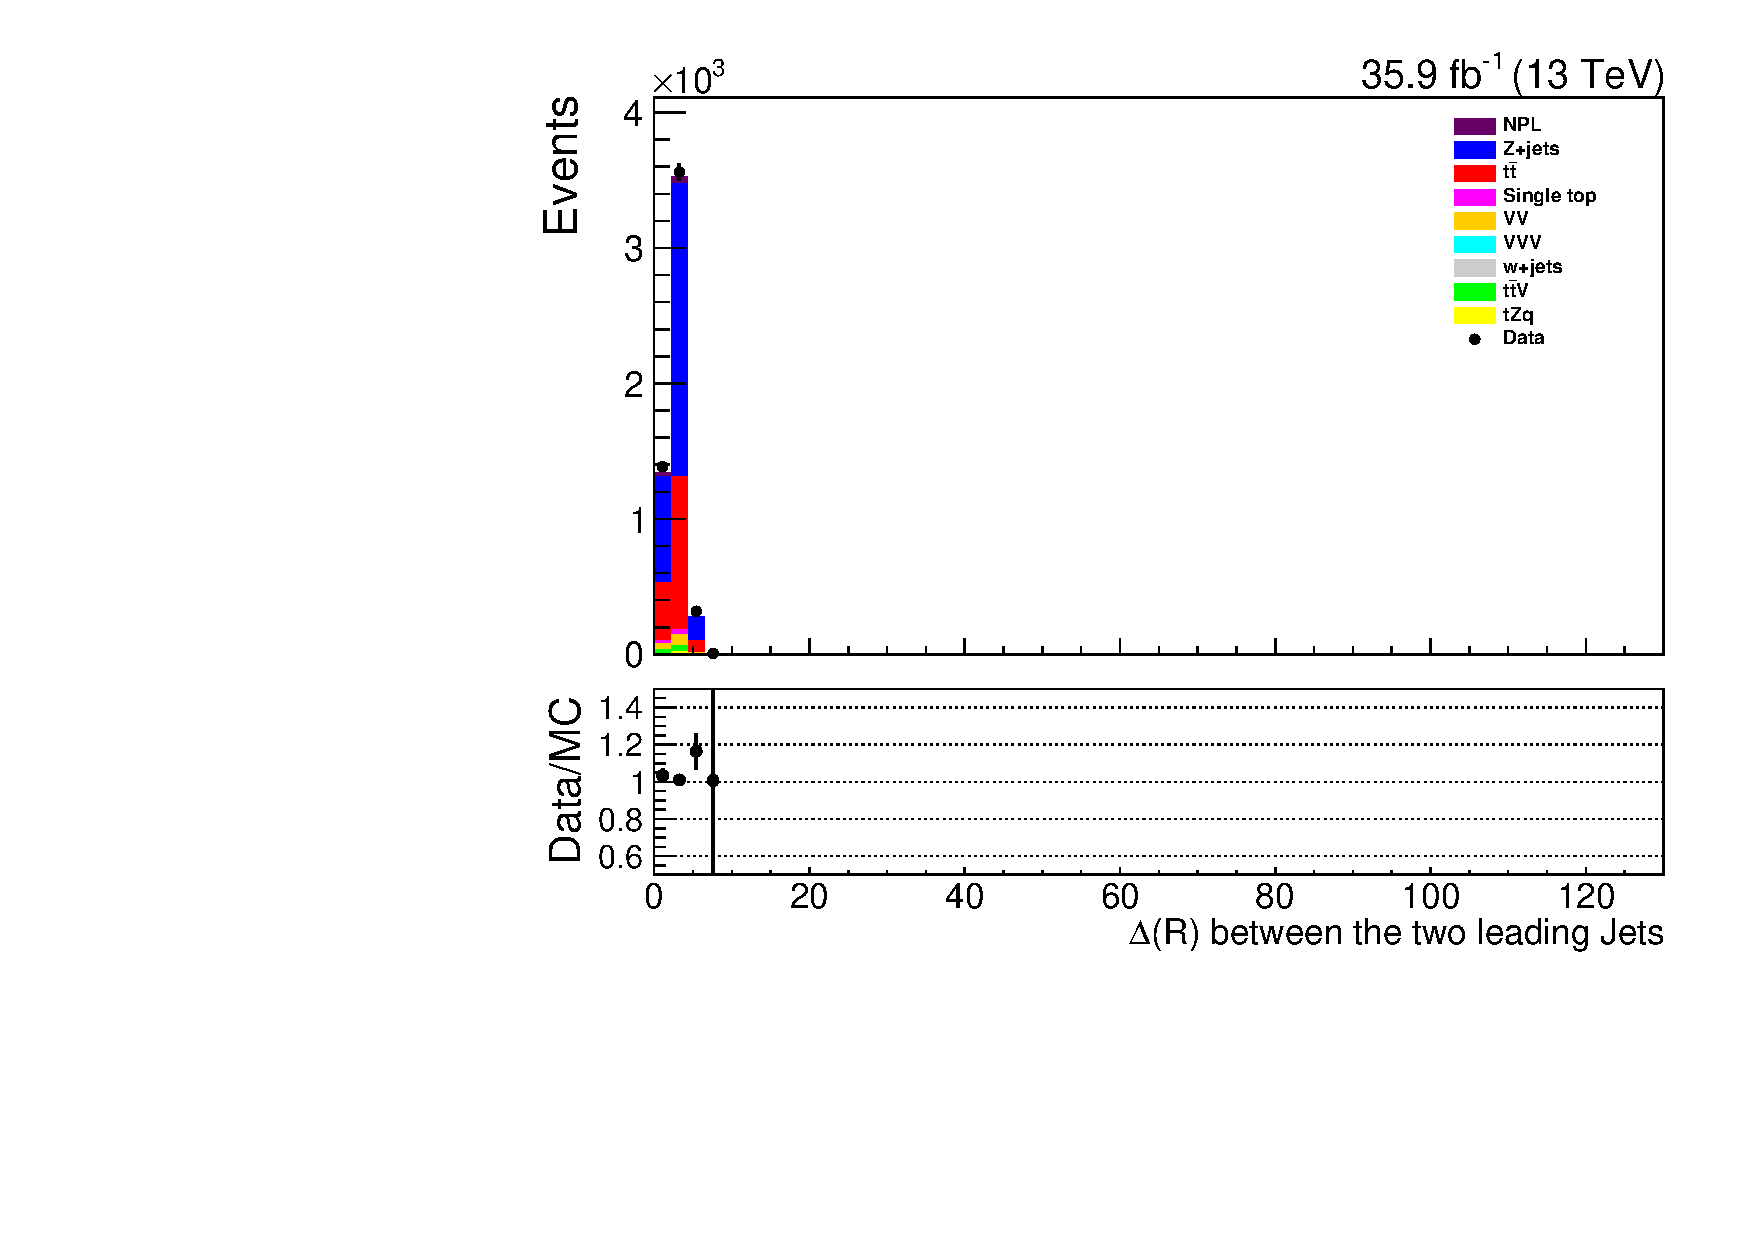
\includegraphics[width=0.47\textwidth]{figs/background-estimation/plots/unblinded/prompt_ee_ttbarInc/jjDelR_NPL_ee_wMass_ee.pdf}
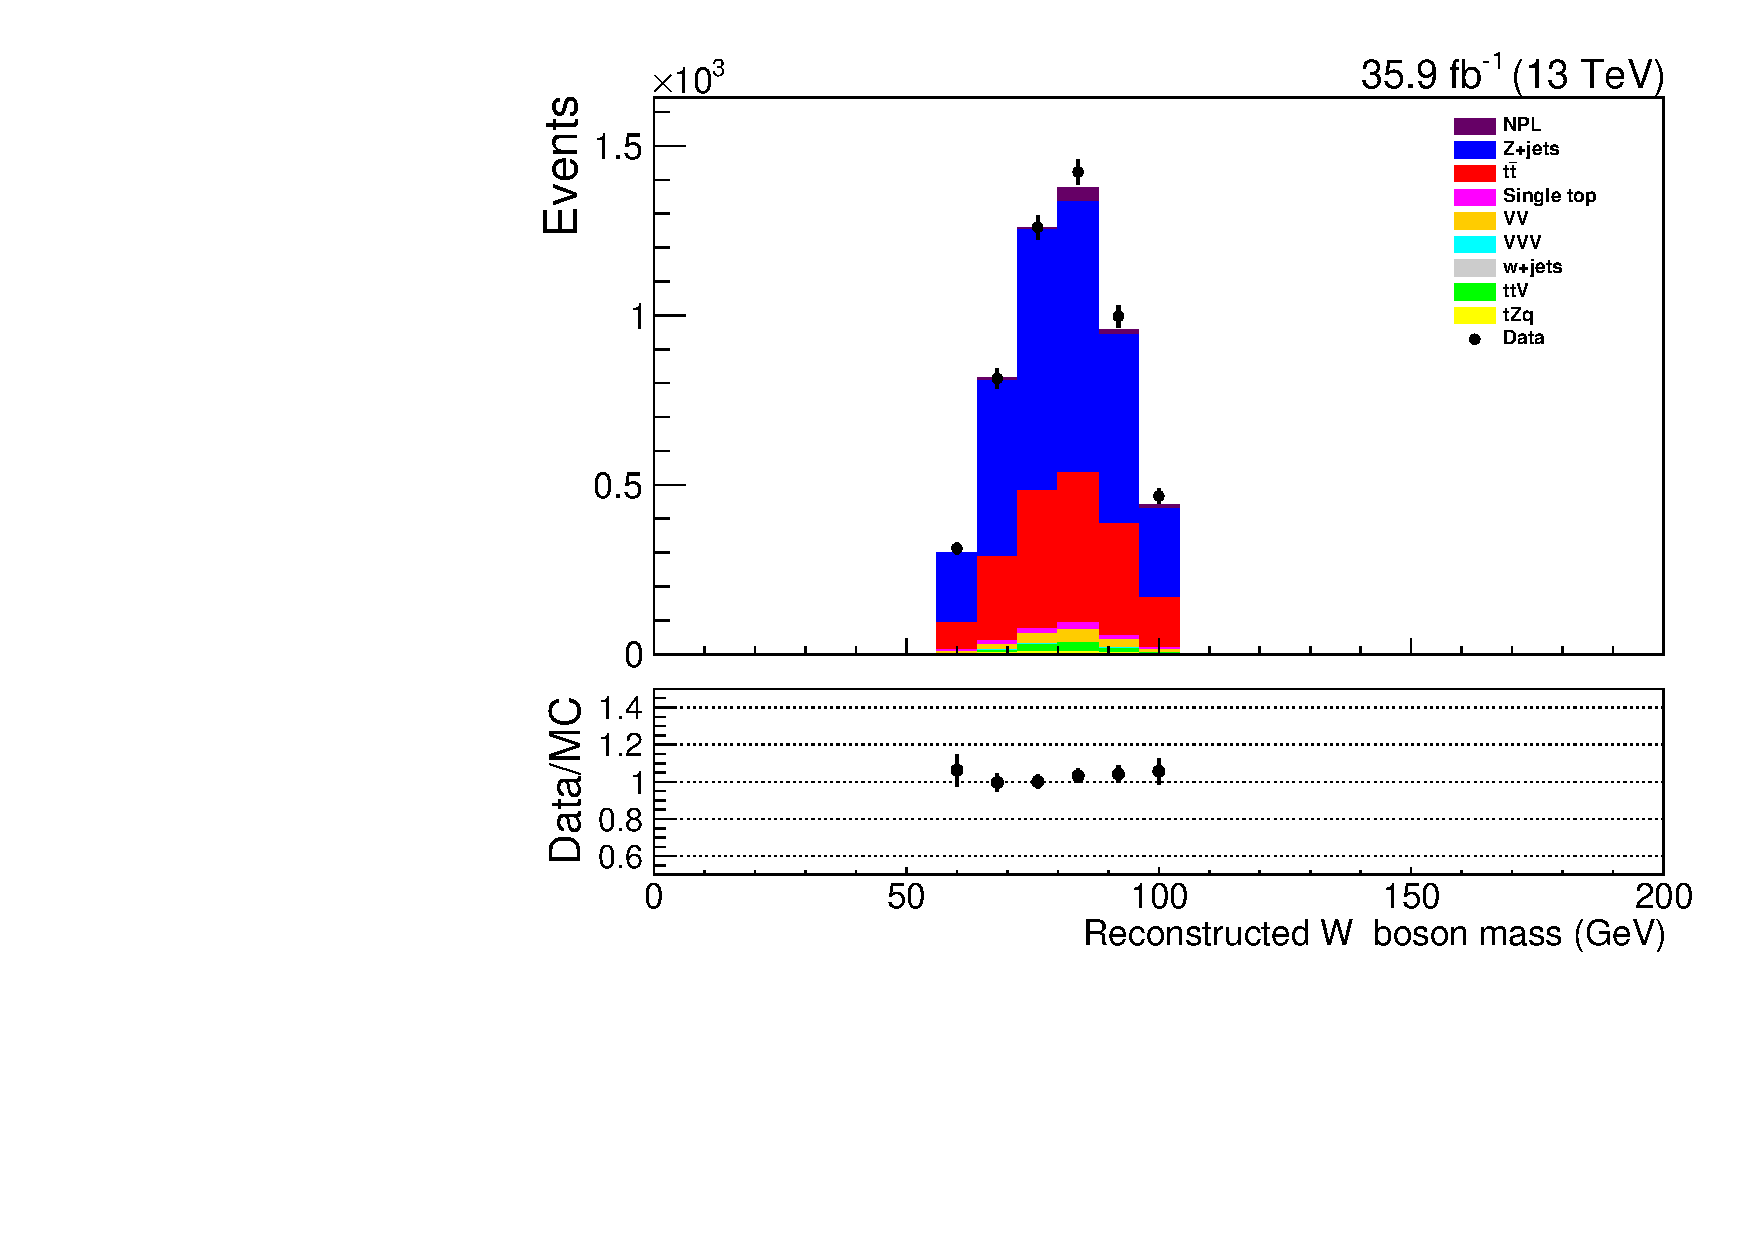
\includegraphics[width=0.47\textwidth]{figs/background-estimation/plots/unblinded/prompt_ee_ttbarInc/wPairMass_NPL_ee_wMass_ee.pdf}
\caption{
Leading b-tagged jet CSVv2 discriminant, leading jet \pT, $\Delta R$ between the leading jets, and reconstructed W boson mass distributions for the $ee$ channel comparing the agreement between data and simulation for the variables used as input variables in the BDT training.}
\label{fig:inputFeaturesDataSimAgreement1}
\end{figure}

\begin{figure}[htb]
\centering
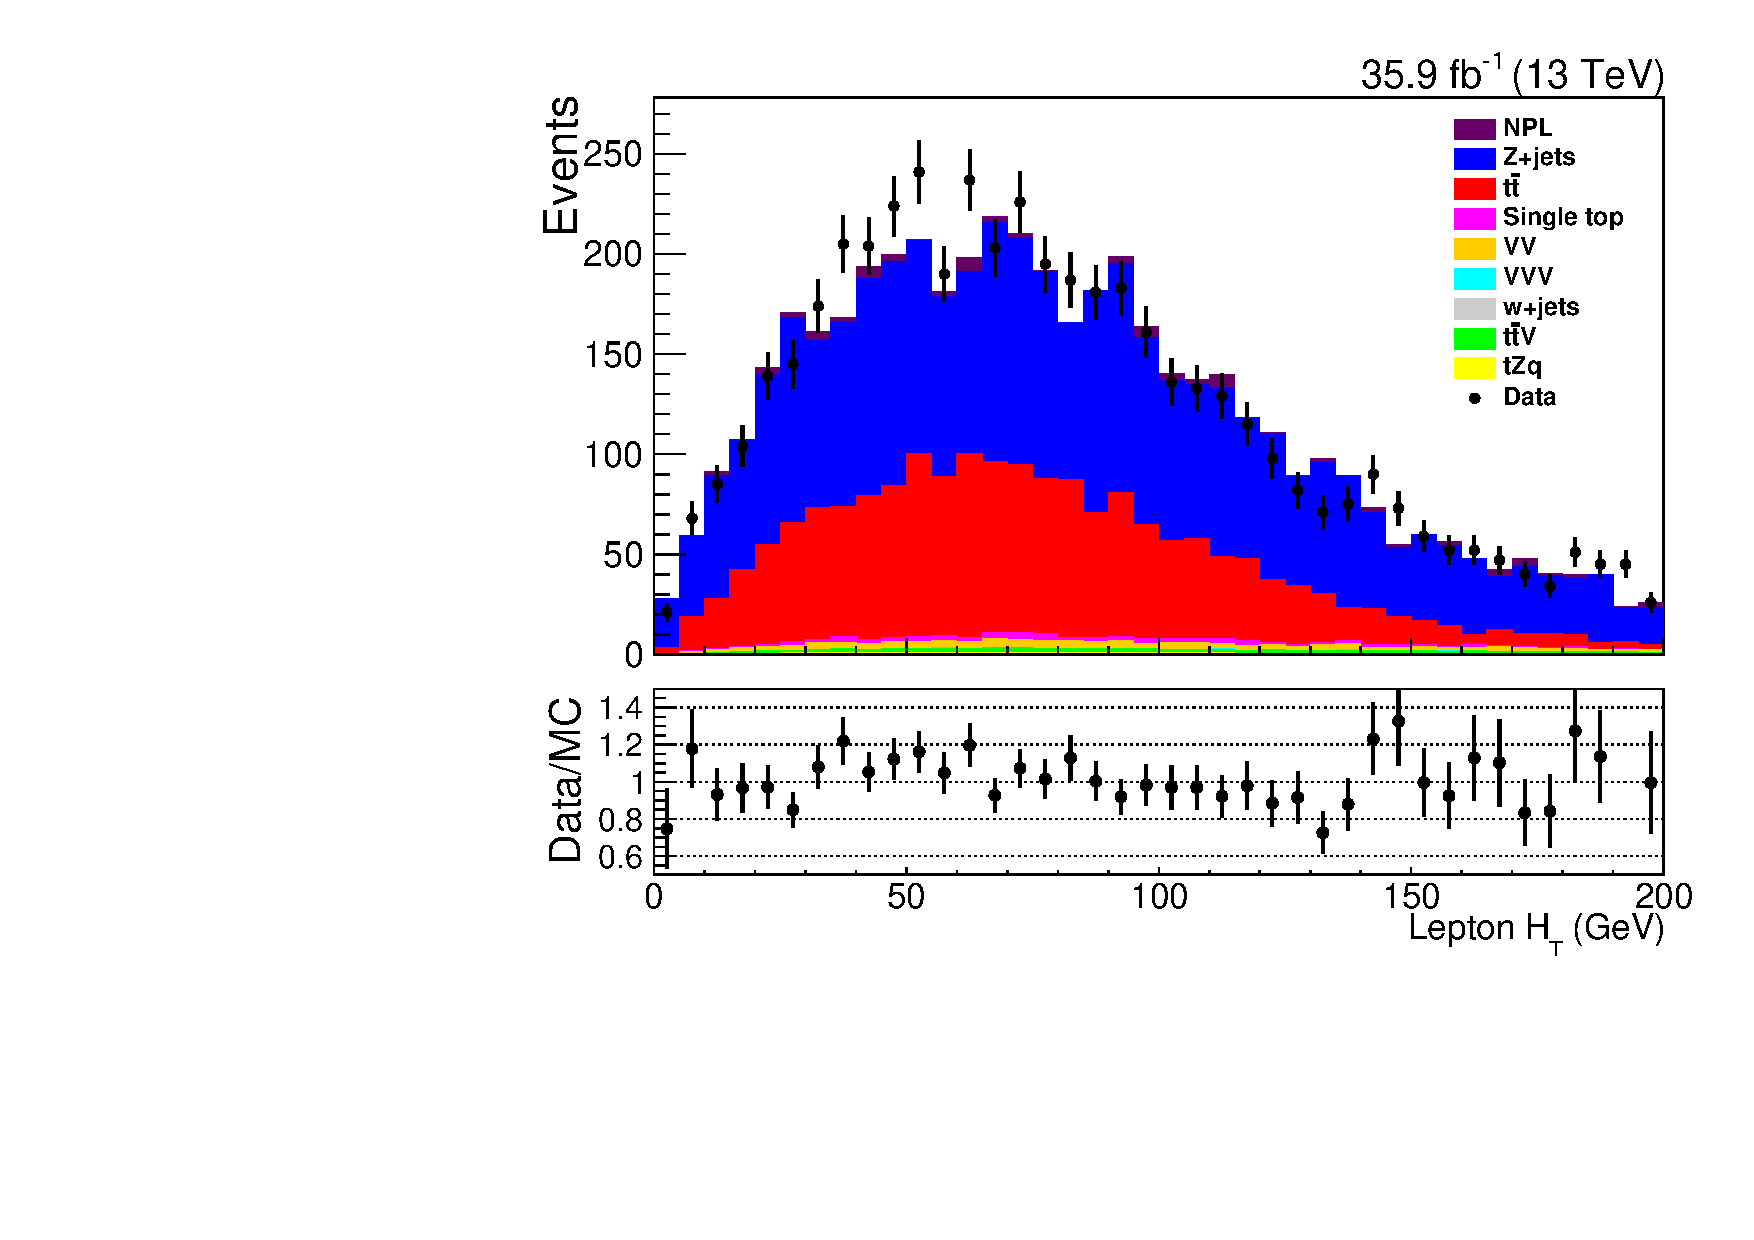
\includegraphics[width=0.47\textwidth]{figs/background-estimation/plots/unblinded/prompt_ee_ttbarInc/lepHt_NPL_ee_wMass_ee.pdf}
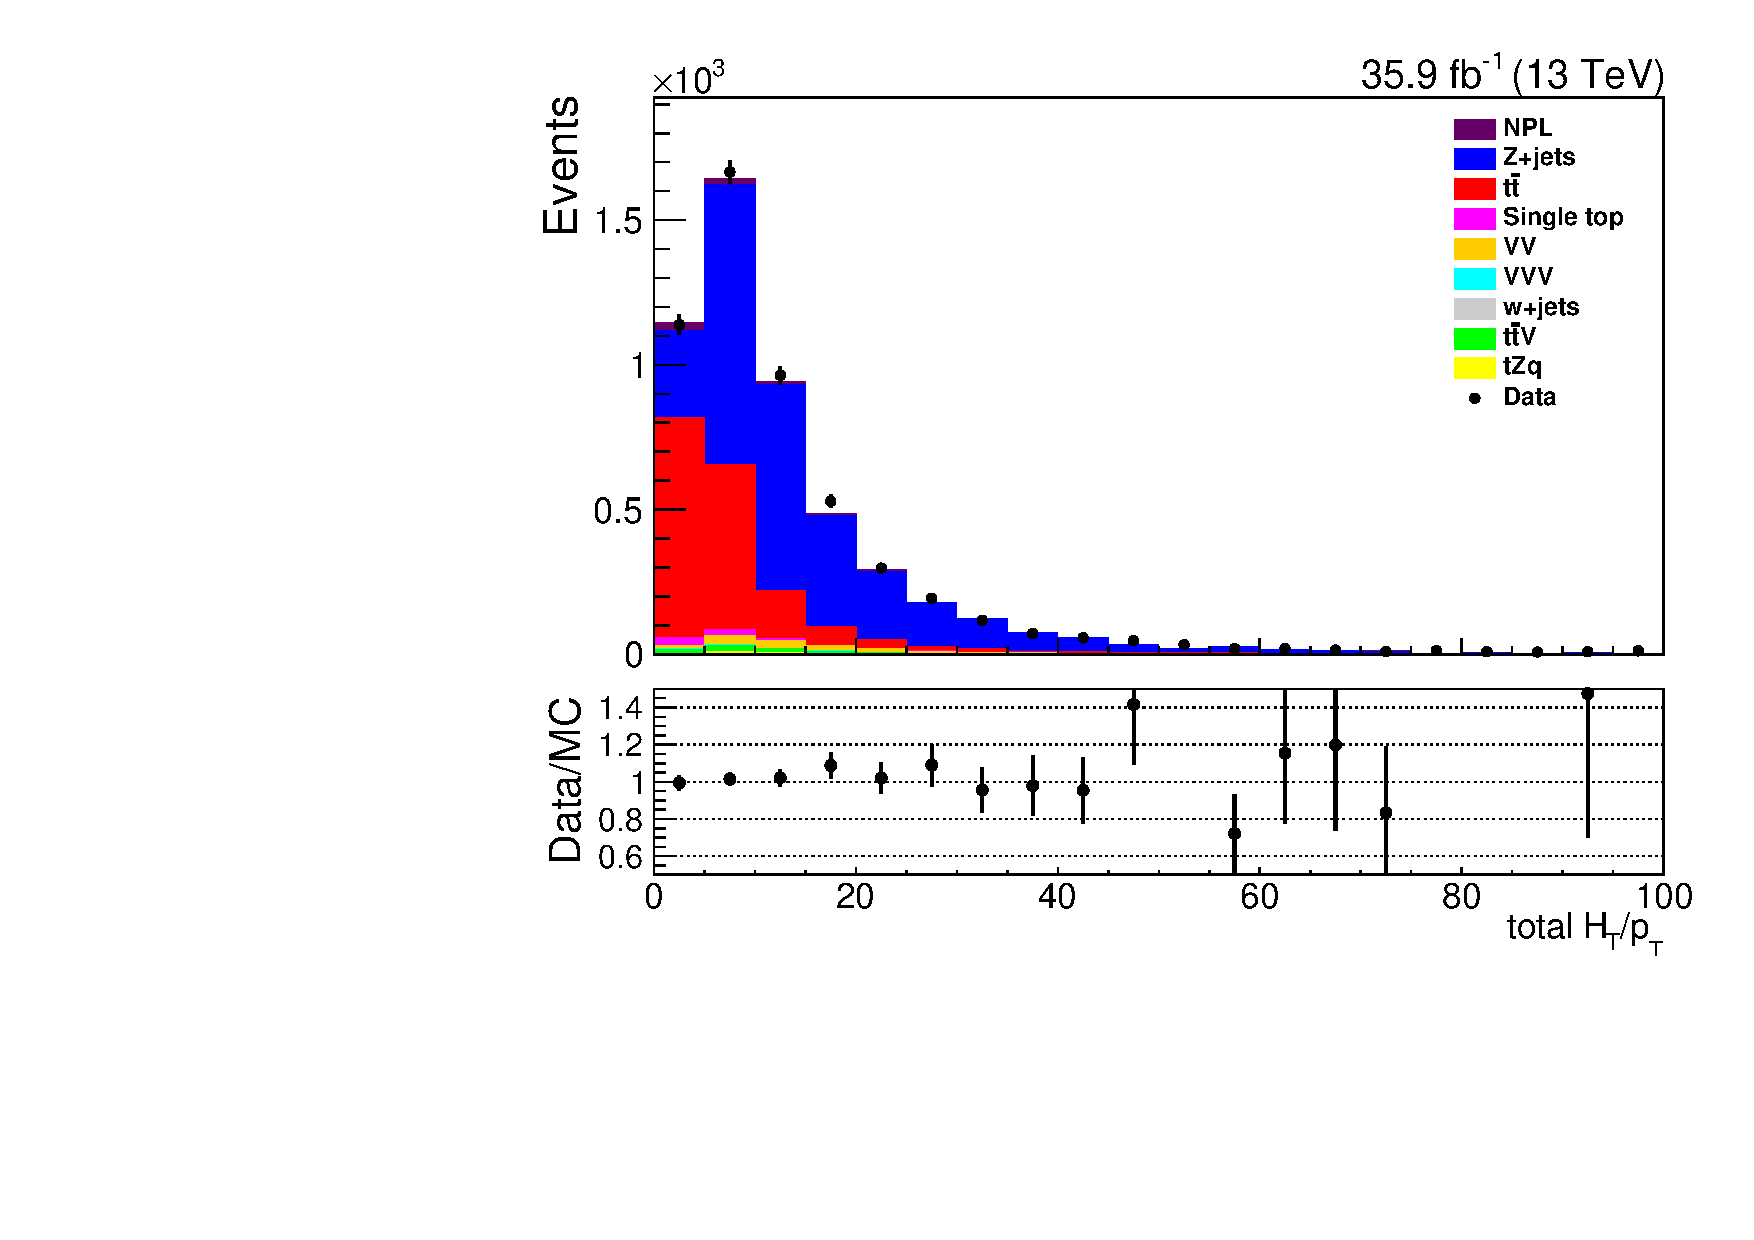
\includegraphics[width=0.47\textwidth]{figs/background-estimation/plots/unblinded/prompt_ee_ttbarInc/totHtOverPt_NPL_ee_wMass_ee.pdf}
\\
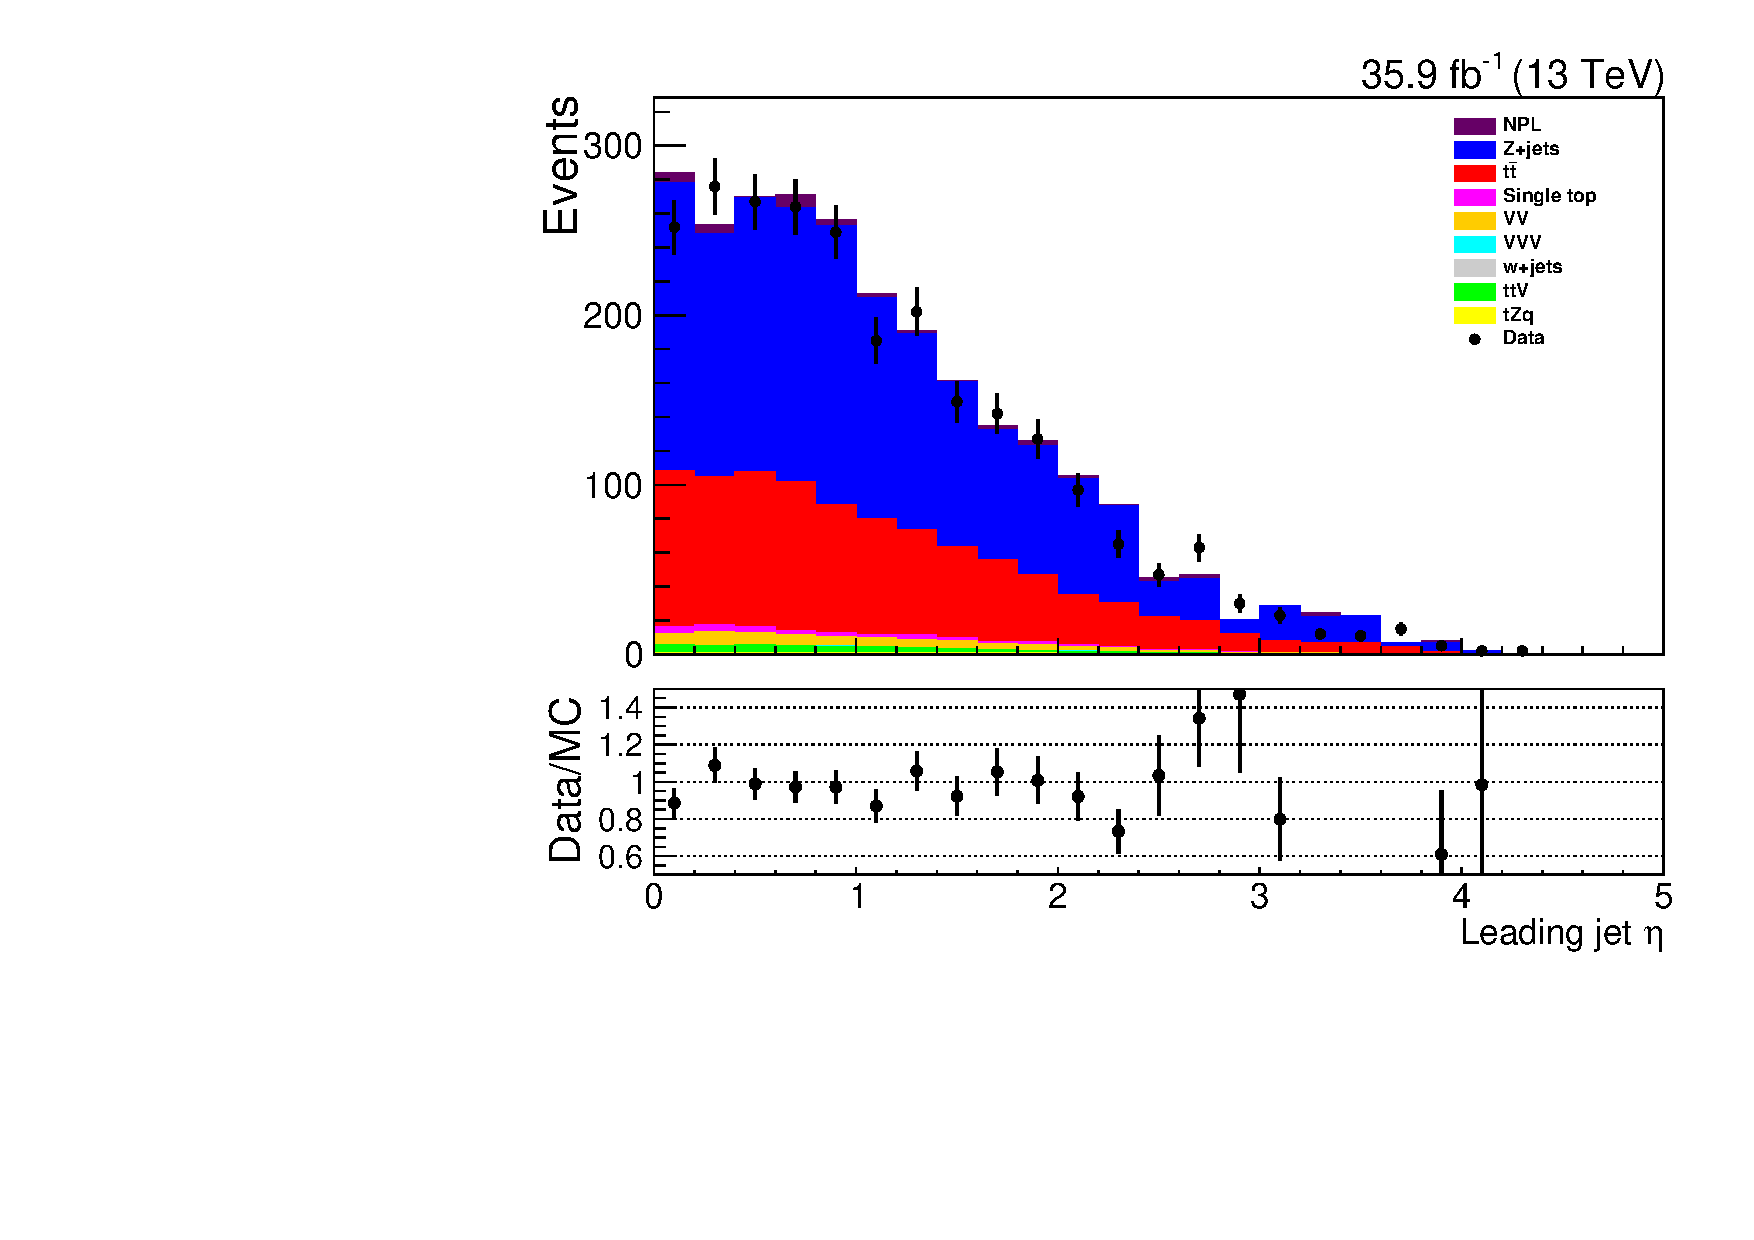
\includegraphics[width=0.47\textwidth]{figs/background-estimation/plots/unblinded/prompt_ee_ttbarInc/leadingJetEta_NPL_ee_wMass_ee.pdf}
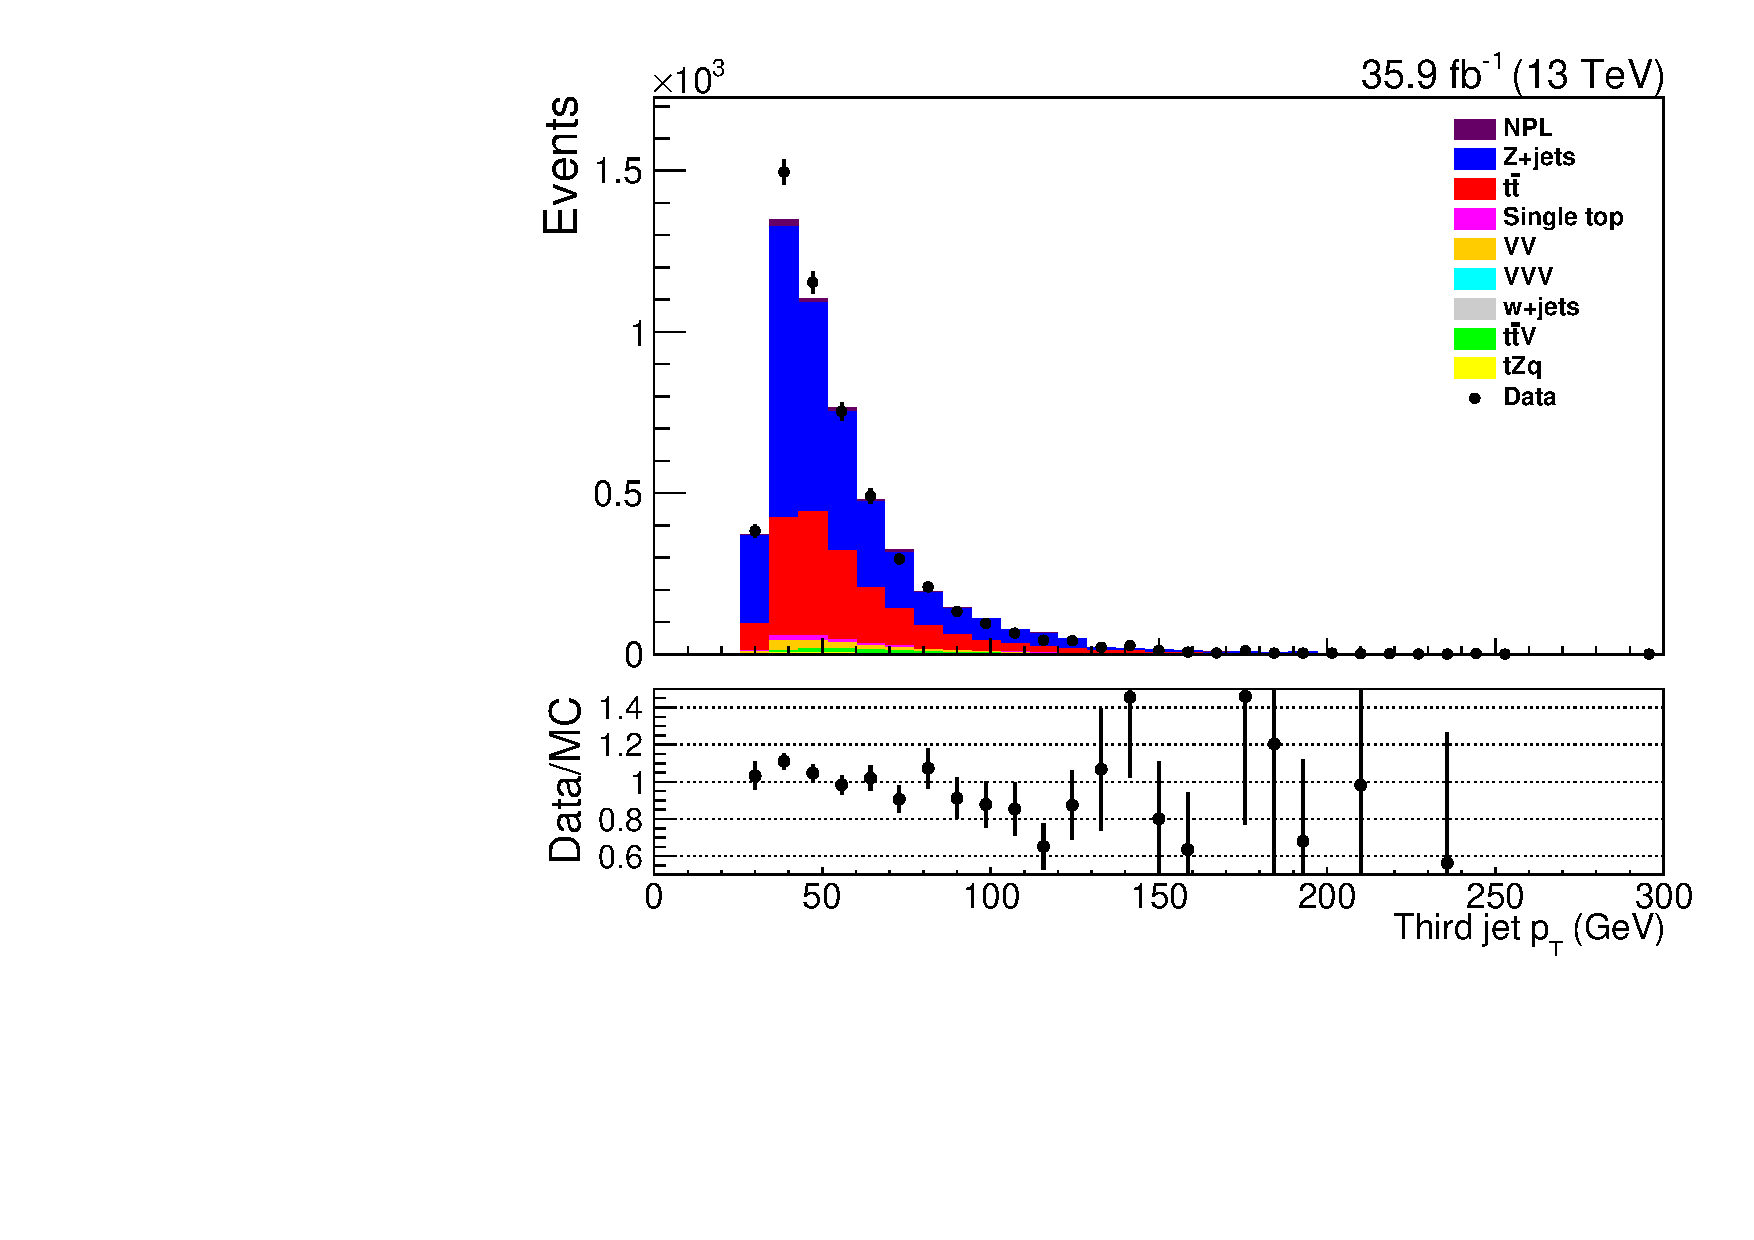
\includegraphics[width=0.47\textwidth]{figs/background-estimation/plots/unblinded/prompt_ee_ttbarInc/thirdJetPt_NPL_ee_wMass_ee.pdf}
\caption{
Lepton ${\ensuremath{H_{\mathrm{T}}}}$, total ${\ensuremath{H_{\mathrm{T}}}}$ divided by total \pt, leading jet $\eta$ and third jet \pT distributions for the $ee$ channel comparing the agreement between data and simulation for the variables used as input variables in the BDT training.}
\label{fig:appInputFeaturesDataSimAgreement2}
\end{figure}

\begin{figure}[htb]
\centering
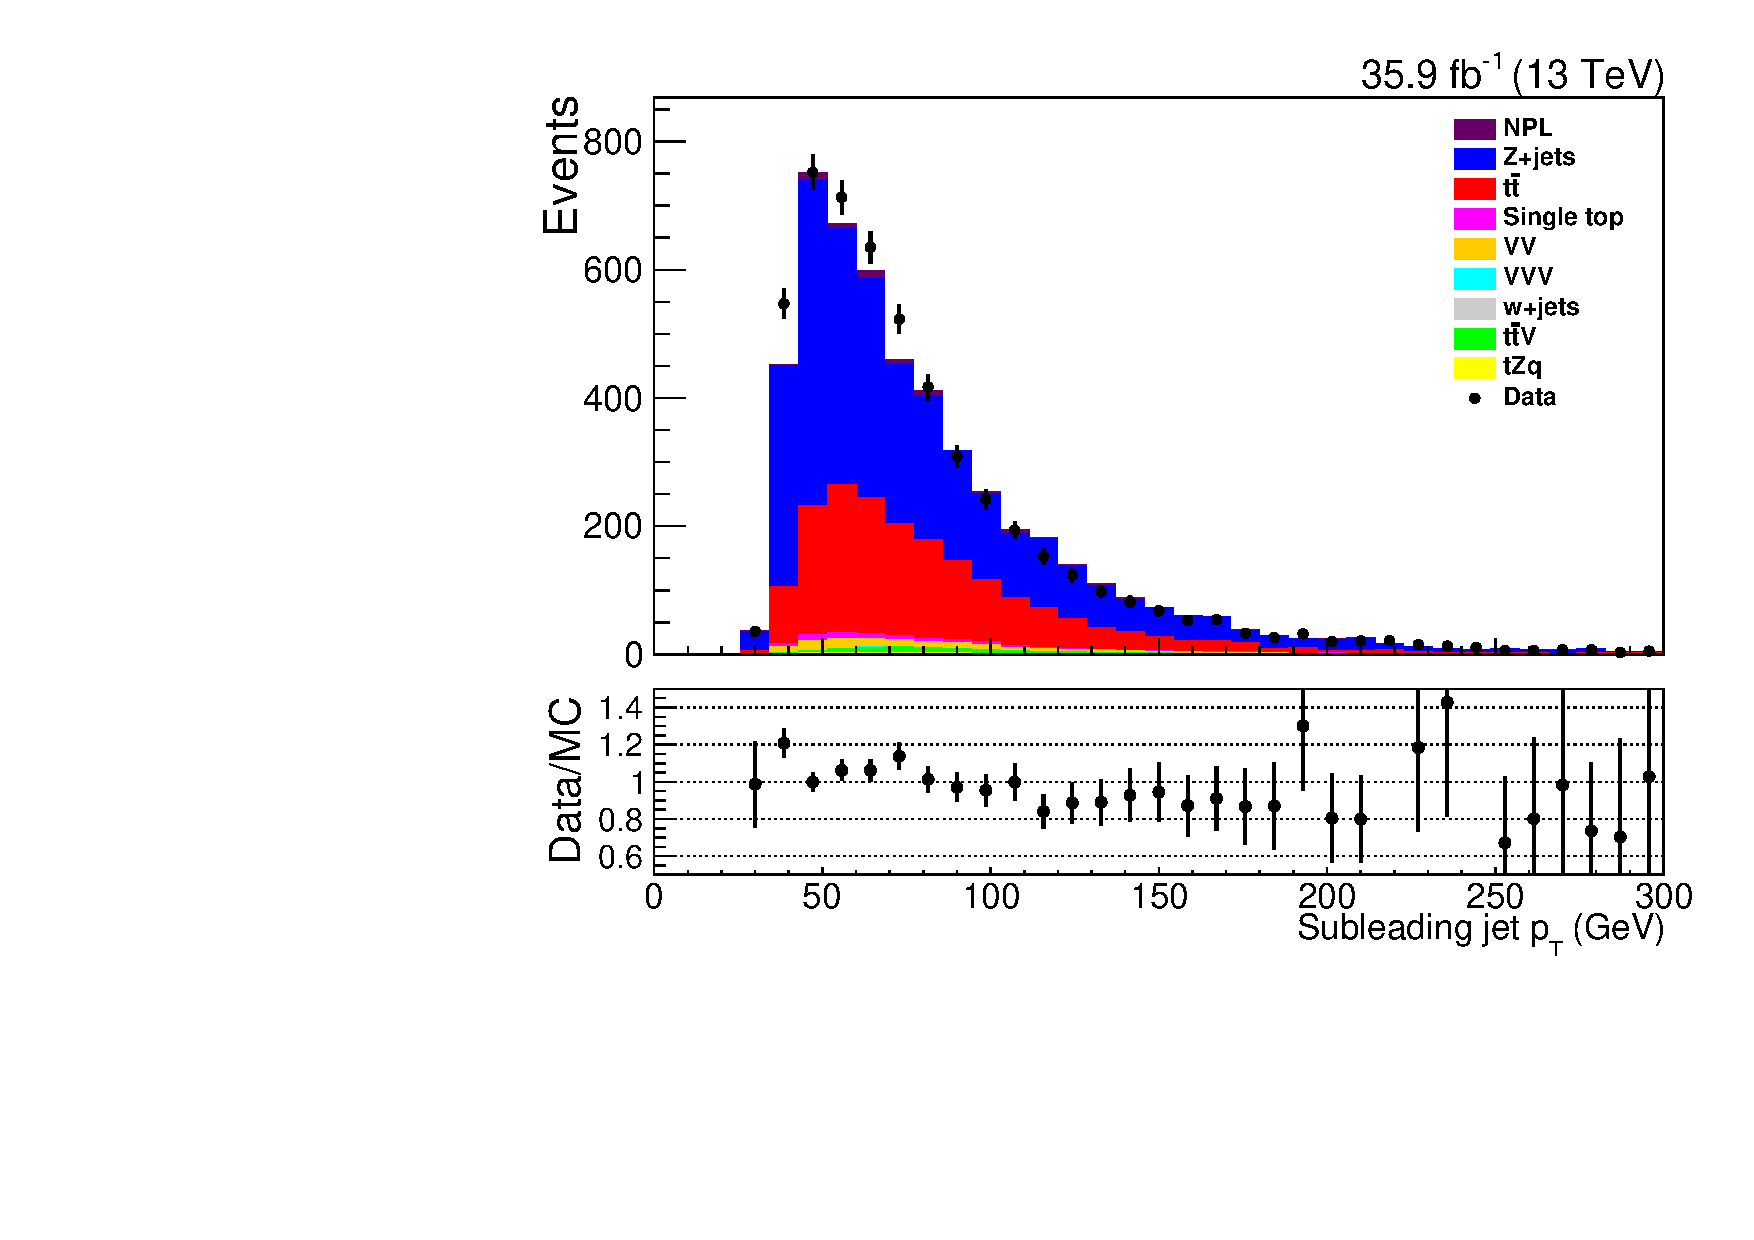
\includegraphics[width=0.47\textwidth]{figs/background-estimation/plots/unblinded/prompt_ee_ttbarInc/secondJetPt_NPL_ee_wMass_ee.pdf}
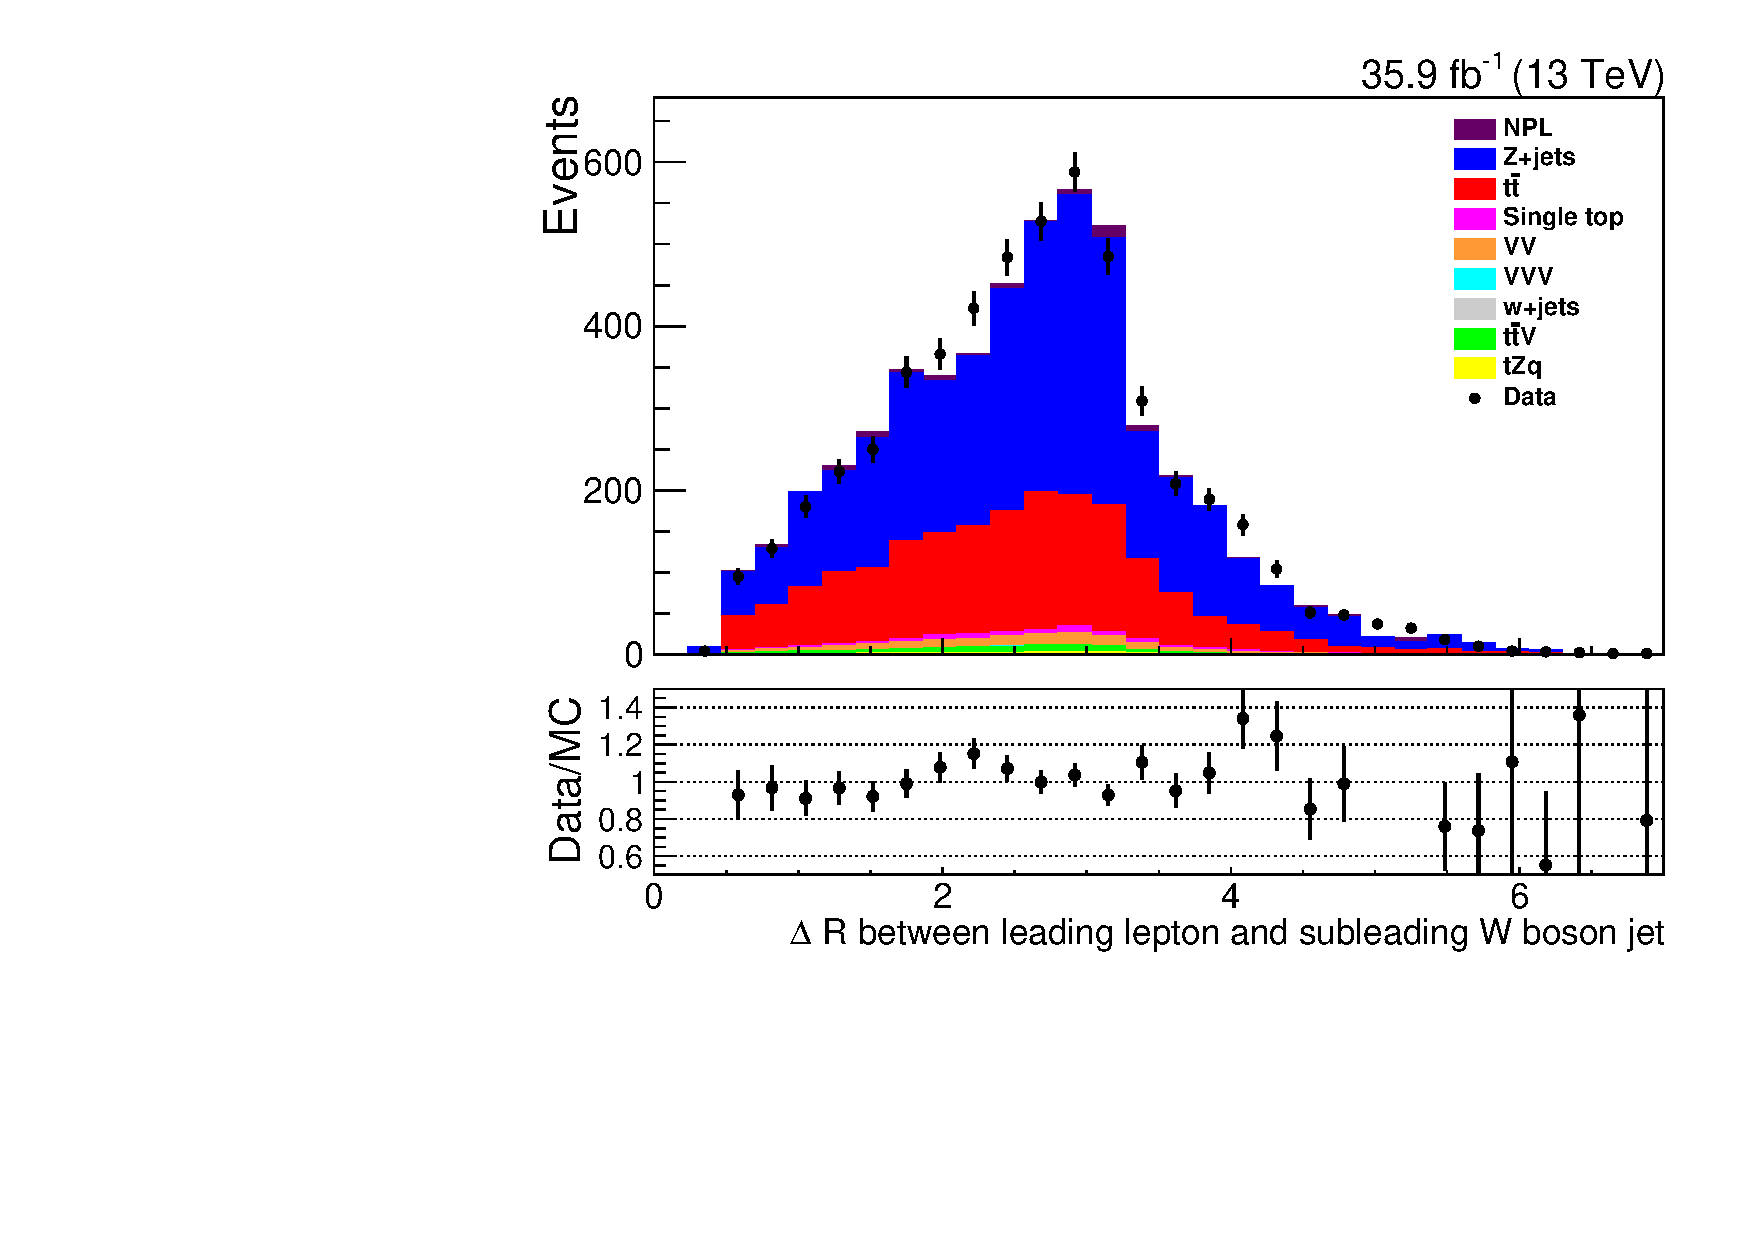
\includegraphics[width=0.47\textwidth]{figs/background-estimation/plots/unblinded/prompt_ee_ttbarInc/zLep1Quark2DelR_NPL_ee_wMass_ee.pdf}
\\
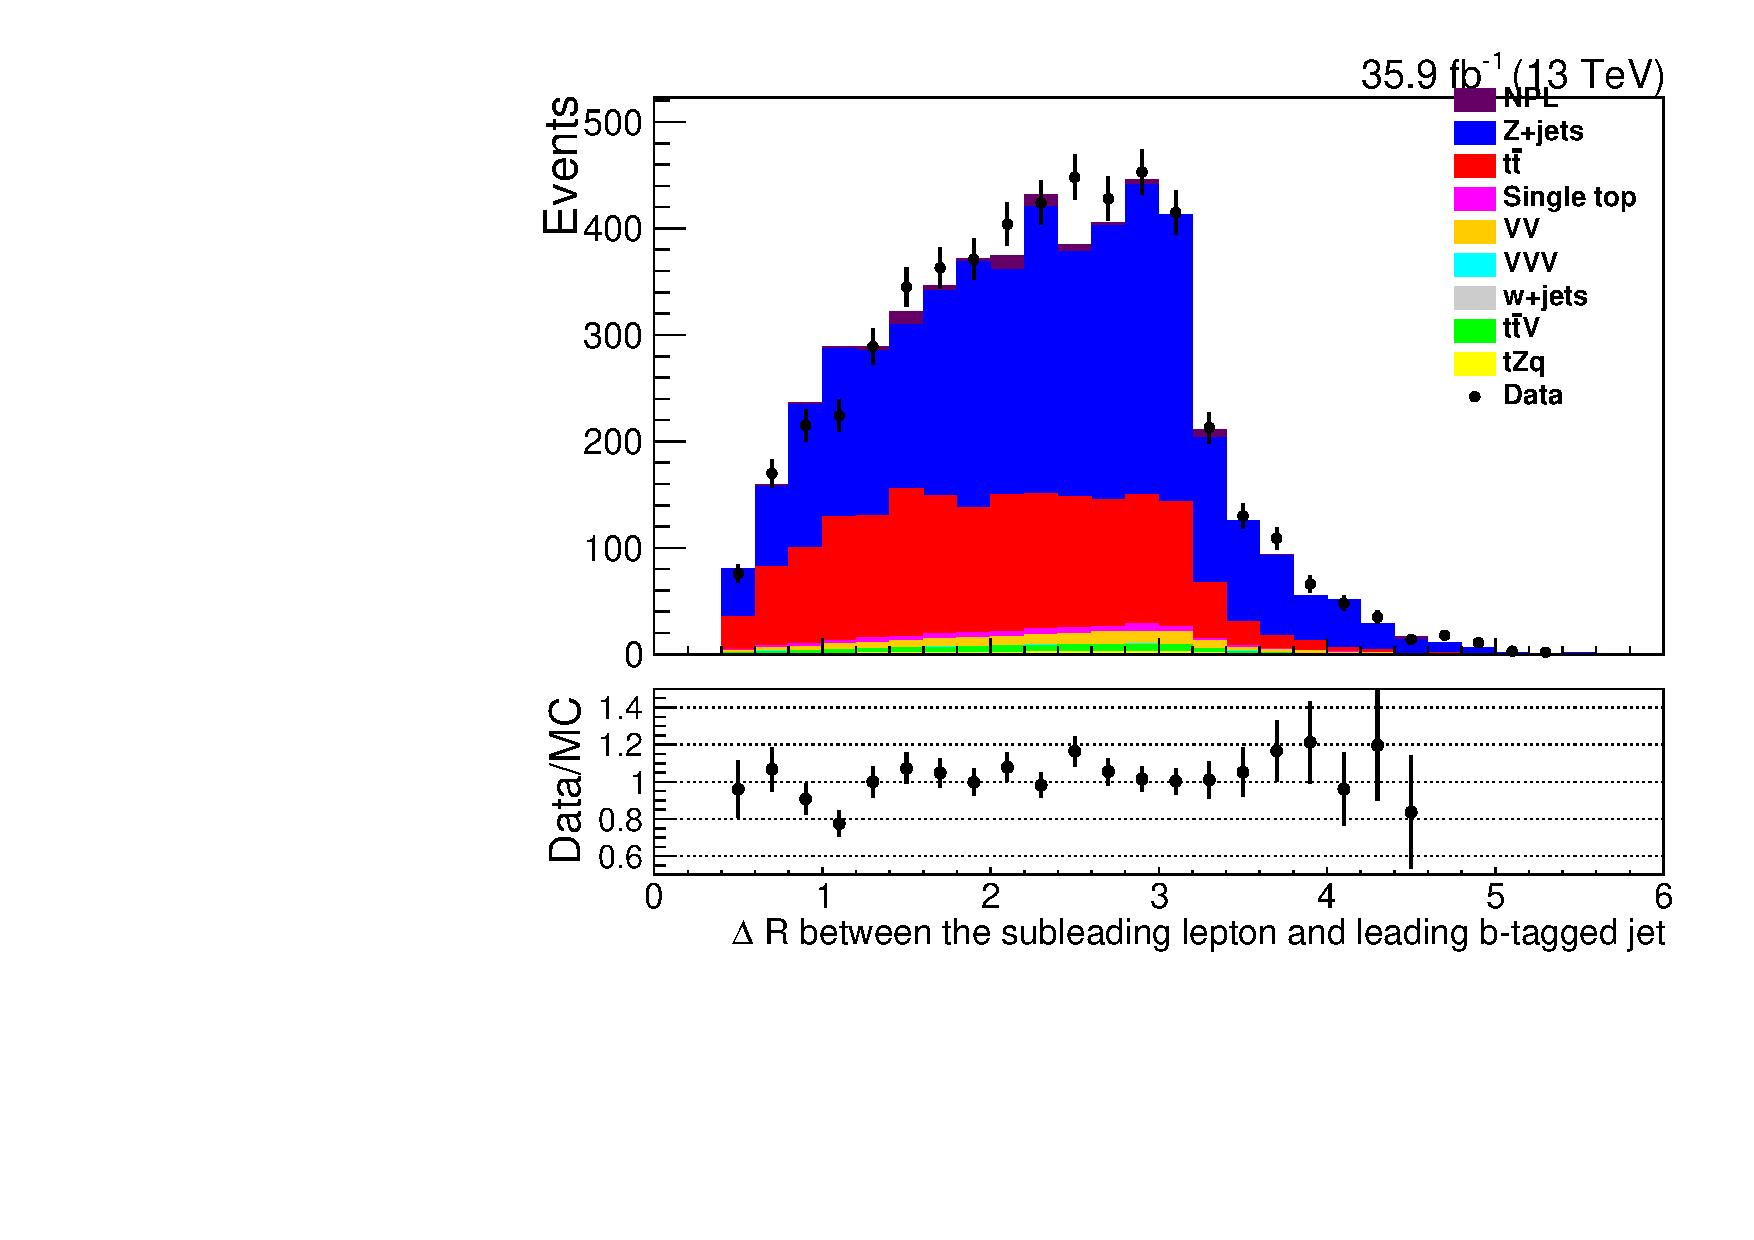
\includegraphics[width=0.47\textwidth]{figs/background-estimation/plots/unblinded/prompt_ee_ttbarInc/zLep2BjetDelR_NPL_ee_wMass_ee.pdf}
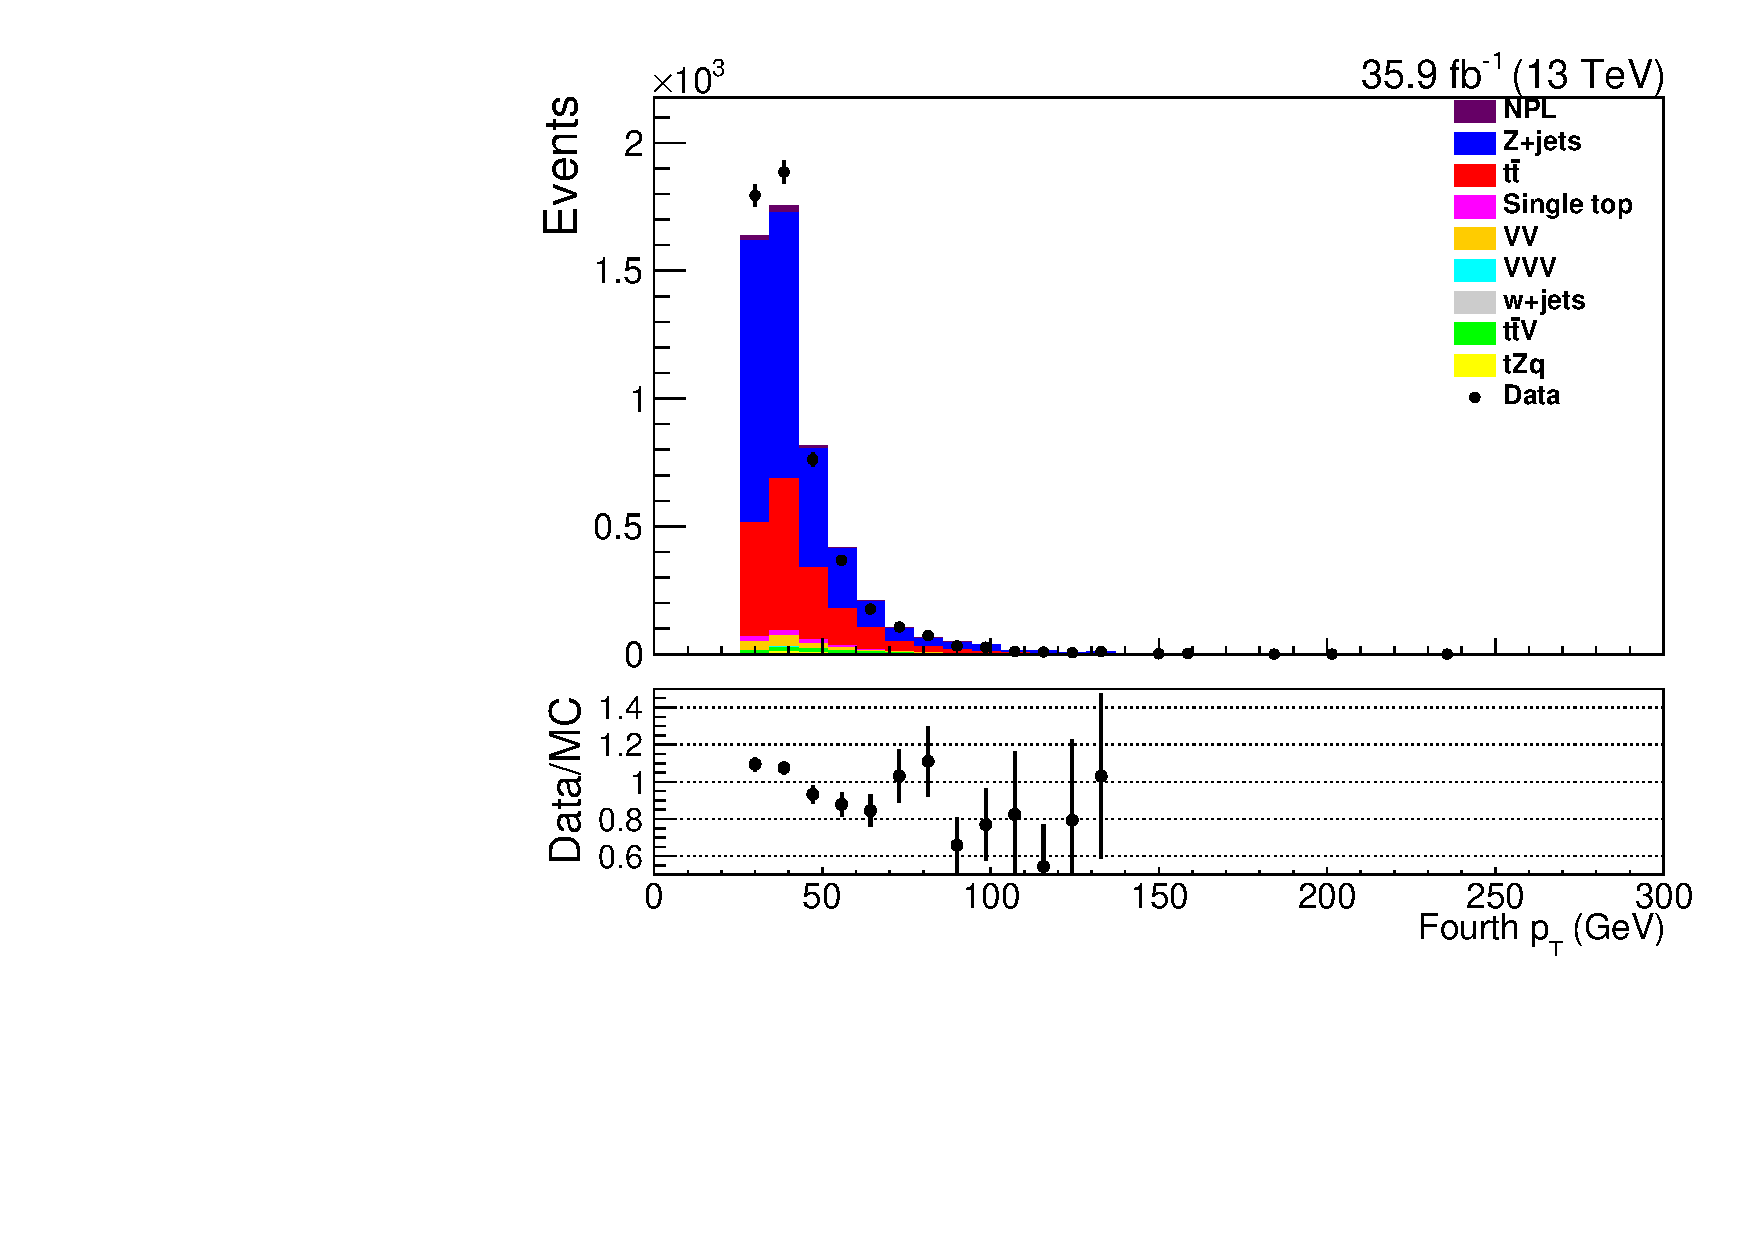
\includegraphics[width=0.47\textwidth]{figs/background-estimation/plots/unblinded/prompt_ee_ttbarInc/fourthJetPt_NPL_ee_wMass_ee.pdf}
\caption{
Second jet \pt, $\Delta R$ between subleading lepton and leading b-tagged jet, $\Delta R$ between subleading lepton and leading b-tagged jet and fourth jet \pT distributions for the $ee$ channel comparing the agreement between data and simulation for the variables used as input variables in the BDT training.}
\label{fig:inputFeaturesDataSimAgreement3}
\end{figure}

\begin{figure}[htb]
\centering
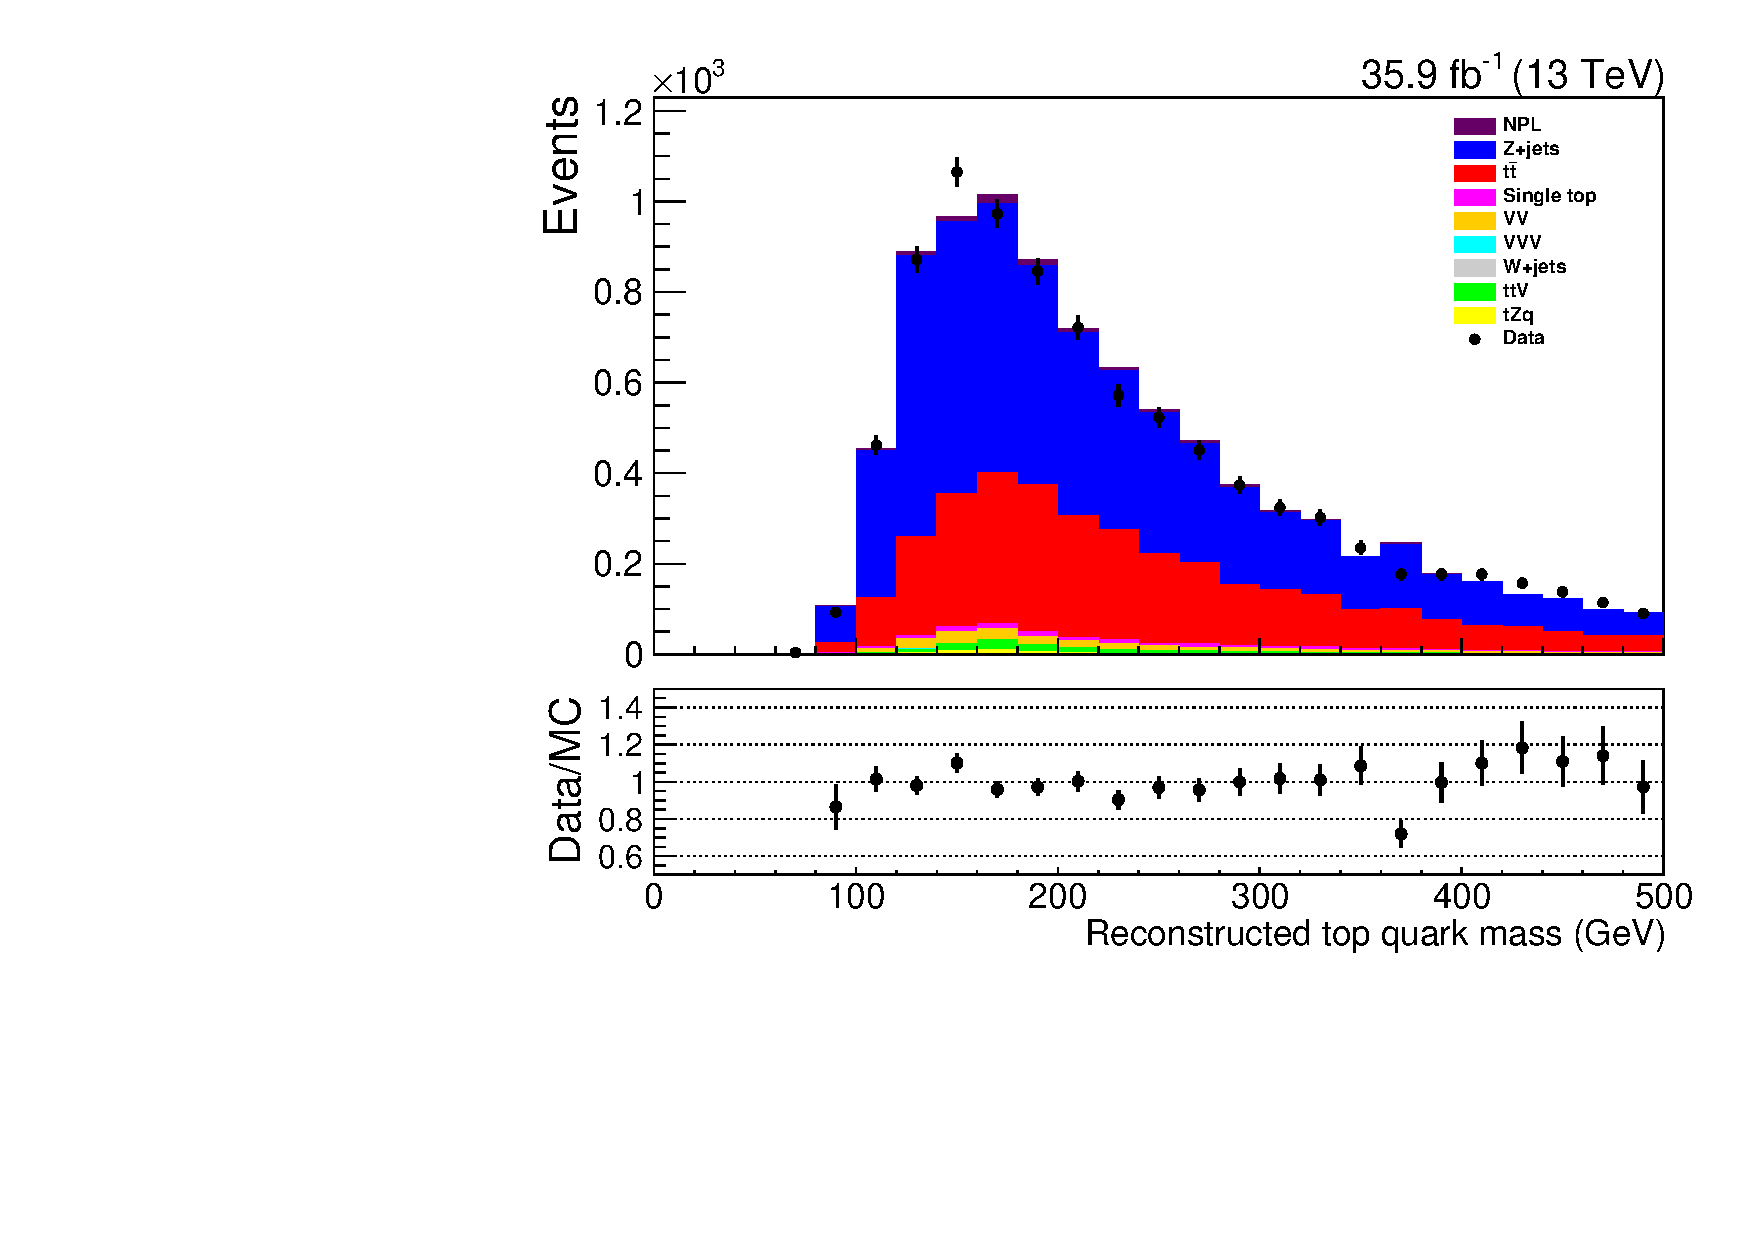
\includegraphics[width=0.47\textwidth]{figs/background-estimation/plots/unblinded/prompt_mumu_ttbarInc/topMass_NPL_mumu_wMass_mumu.pdf}
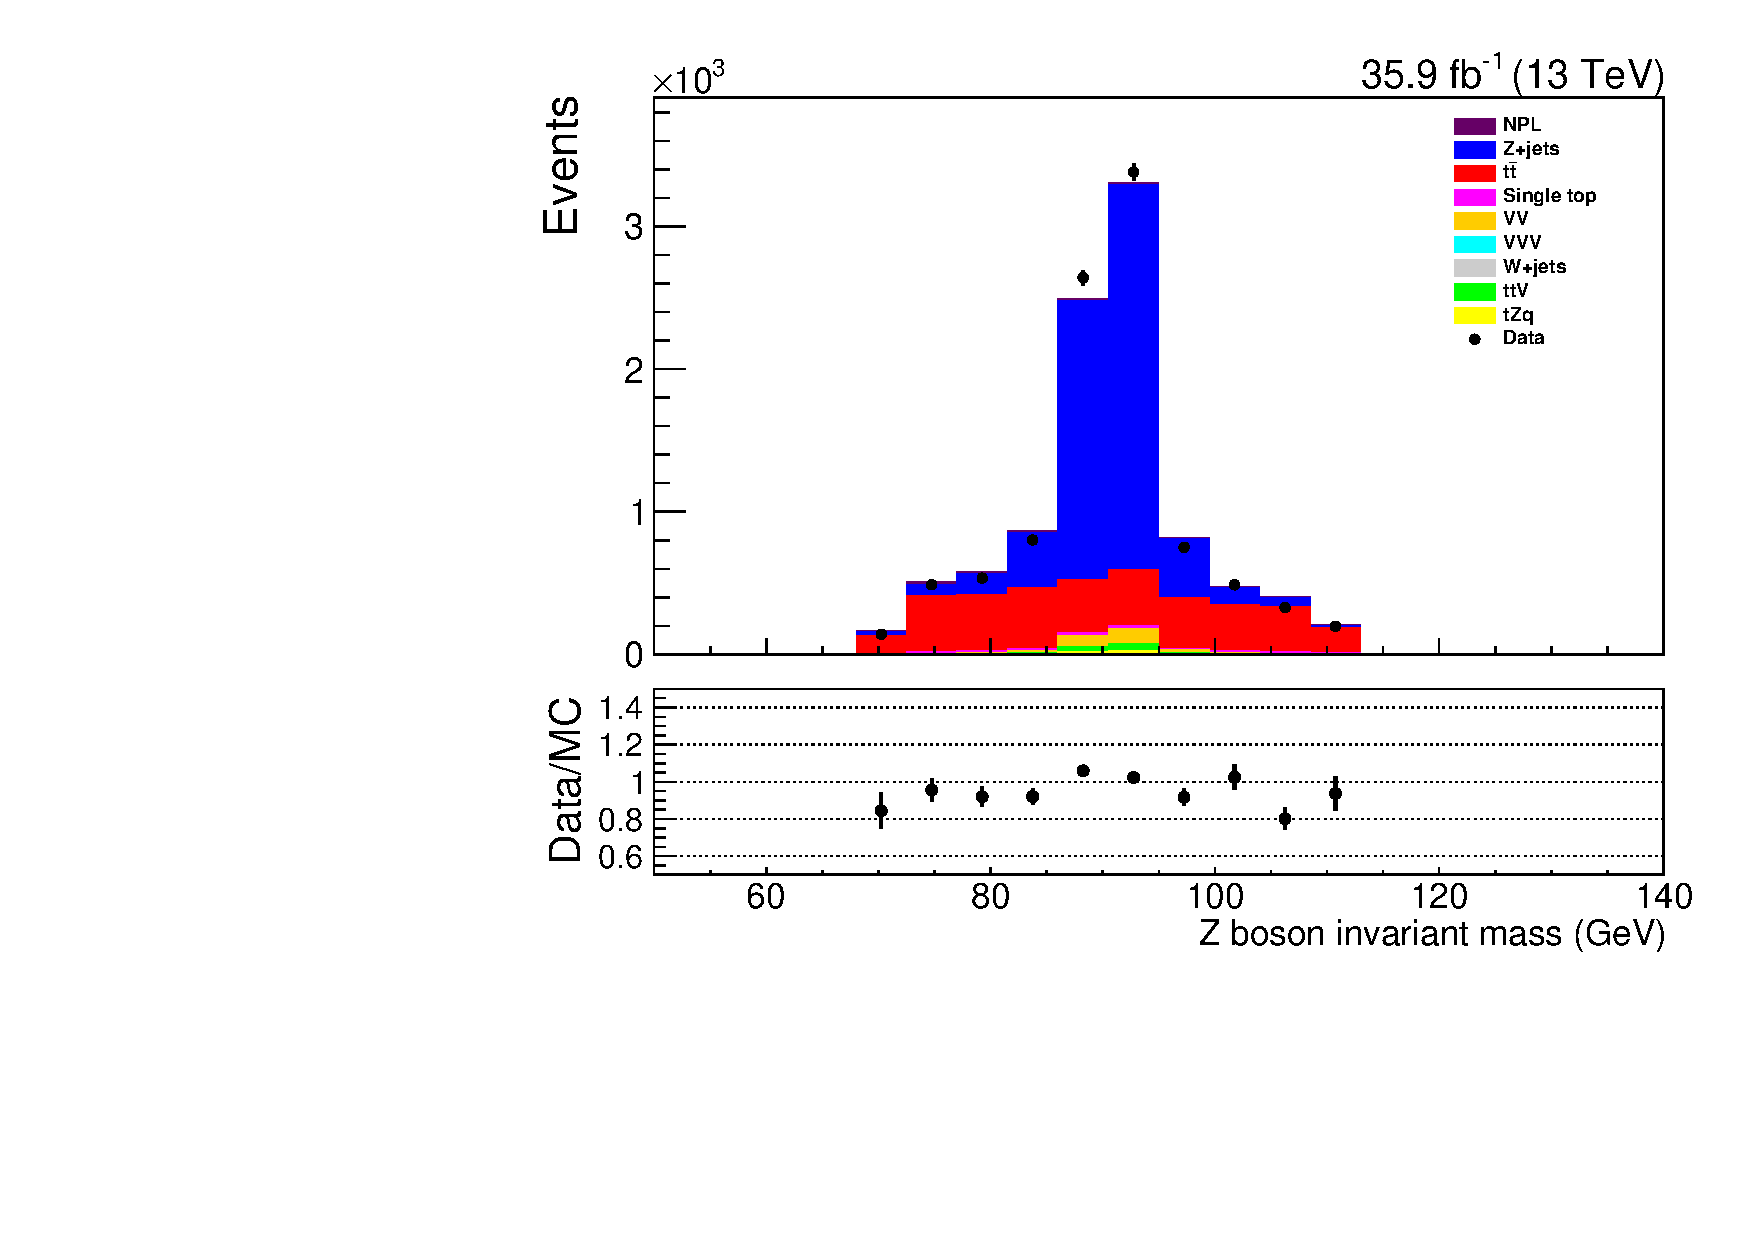
\includegraphics[width=0.47\textwidth]{figs/background-estimation/plots/unblinded/prompt_mumu_ttbarInc/zPairMass_NPL_mumu_wMass_mumu.pdf}
\\
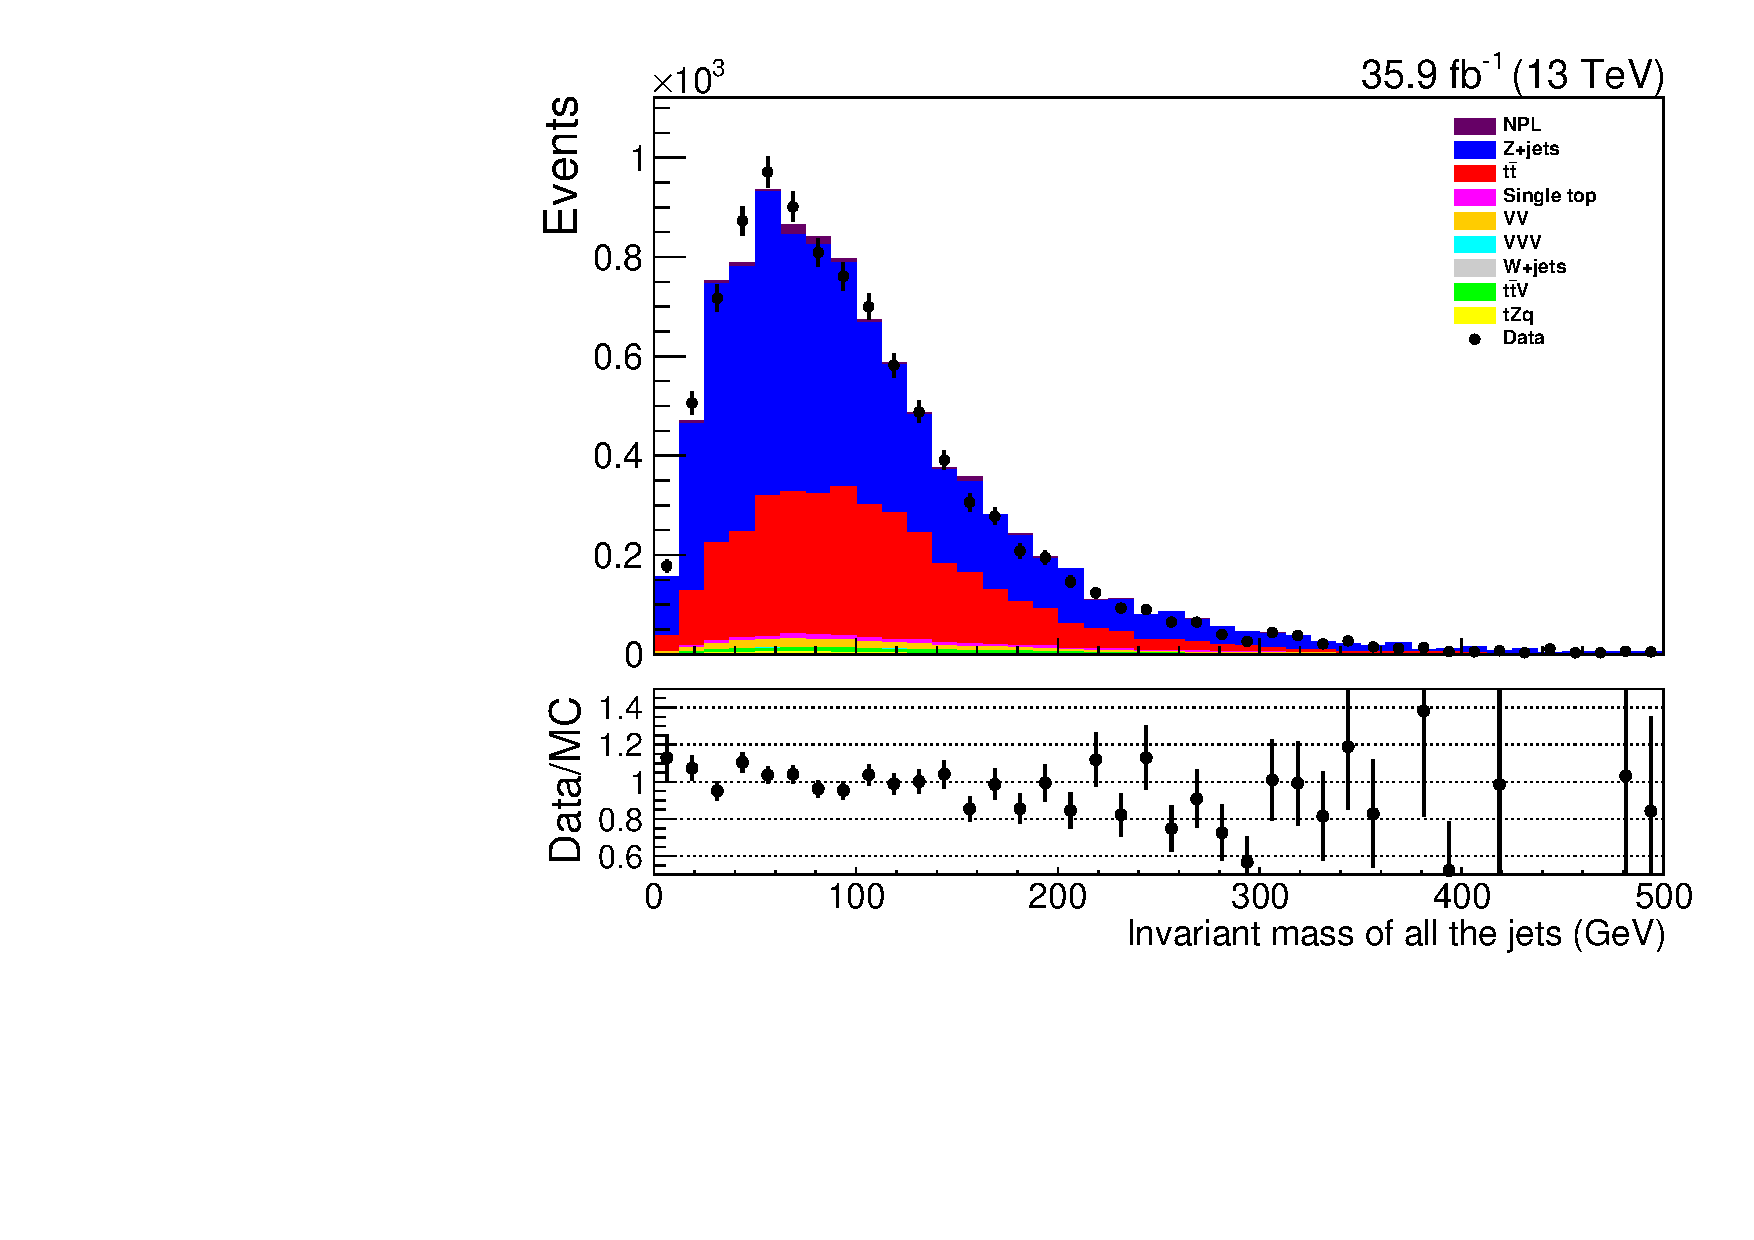
\includegraphics[width=0.47\textwidth]{figs/background-estimation/plots/unblinded/prompt_mumu_ttbarInc/totalJetMass_NPL_mumu_wMass_mumu.pdf}
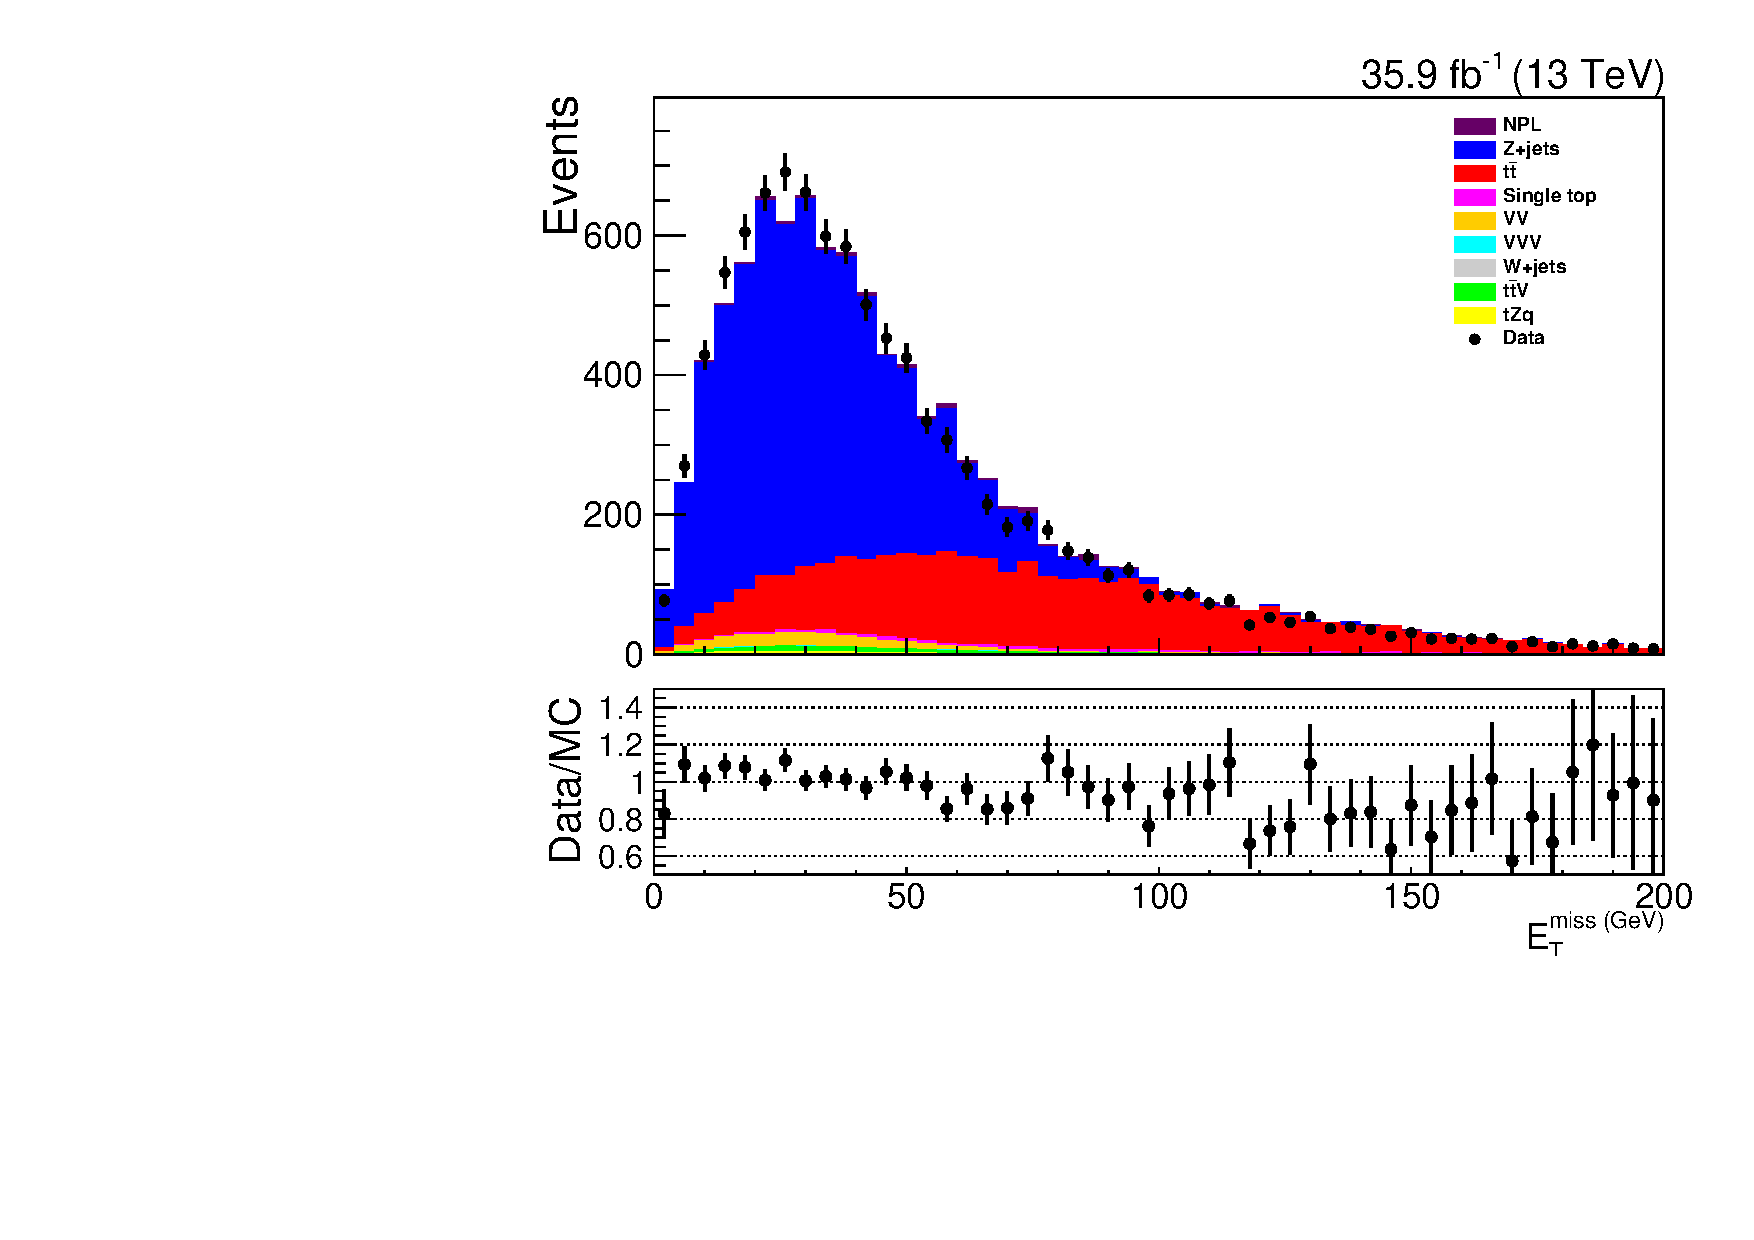
\includegraphics[width=0.47\textwidth]{figs/background-estimation/plots/unblinded/prompt_mumu_ttbarInc/met_NPL_mumu_wMass_mumu.pdf}
\caption{
Reconstructed top mass, Z boson mass, total jet mass, and \MET distributions for the $\mu\mu$ channel comparing the agreement between data and simulation for the variables used as input variables in the BDT training.}
\label{fig:appInputFeaturesDataSimAgreement10}
\end{figure}

\begin{figure}[htb]
\centering
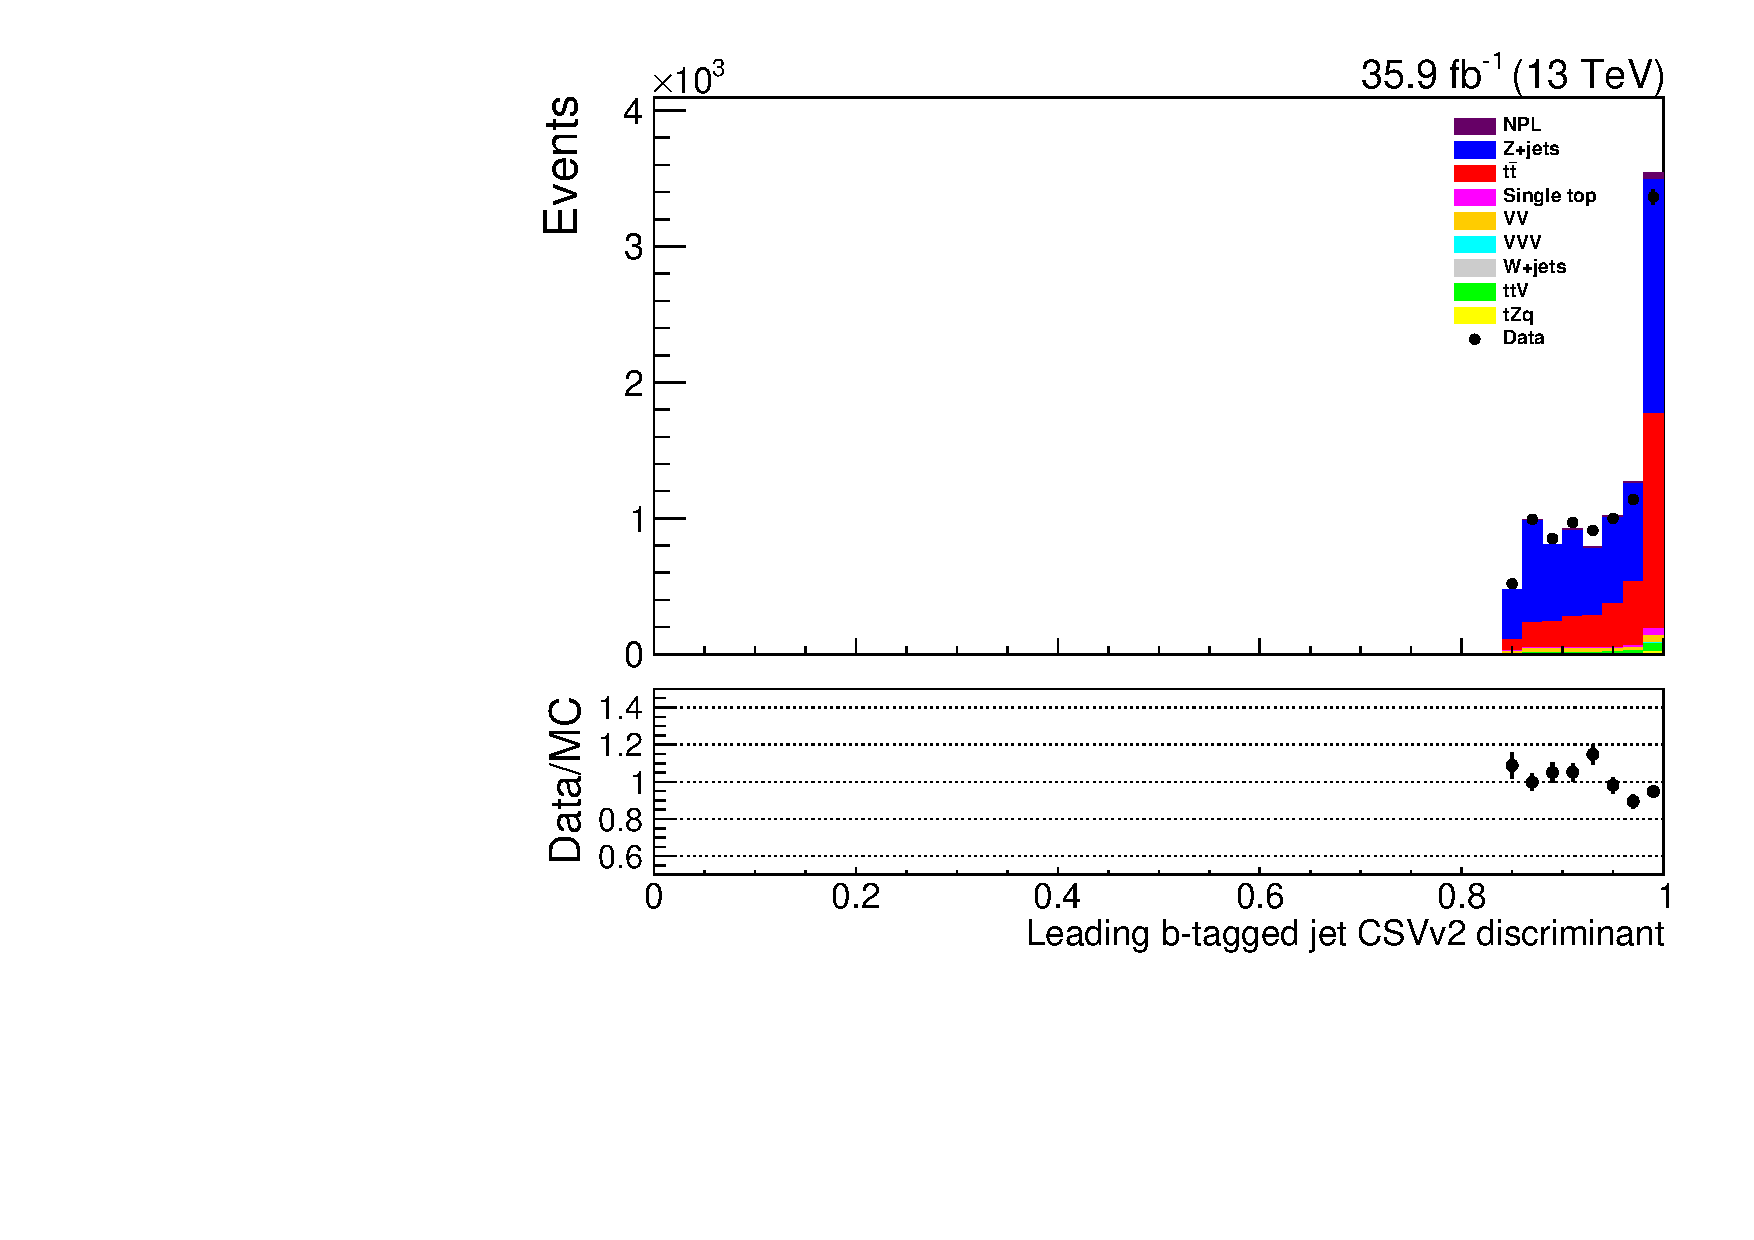
\includegraphics[width=0.47\textwidth]{figs/background-estimation/plots/unblinded/prompt_mumu_ttbarInc/bTagDisc_NPL_mumu_wMass_mumu.pdf}
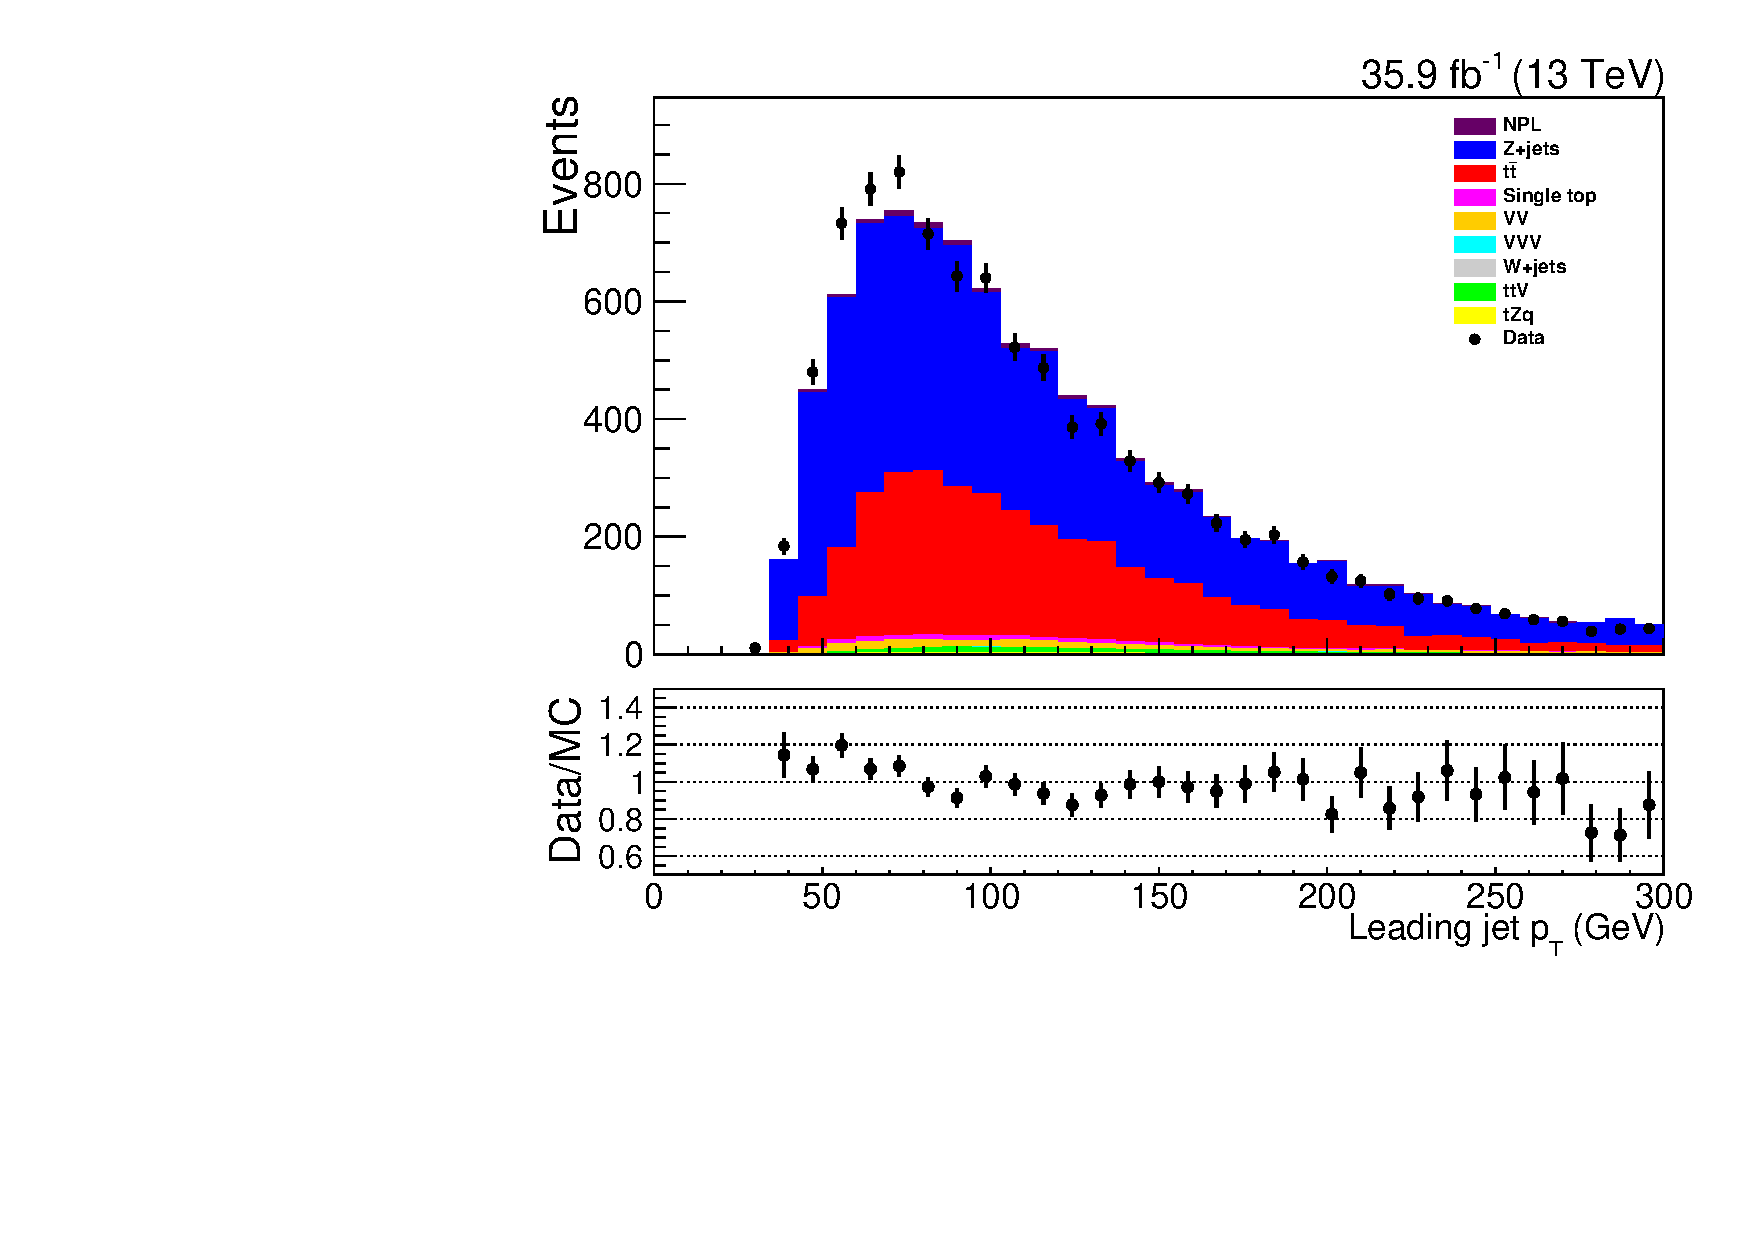
\includegraphics[width=0.47\textwidth]{figs/background-estimation/plots/unblinded/prompt_mumu_ttbarInc/leadingJetPt_NPL_mumu_wMass_mumu.pdf}
\\
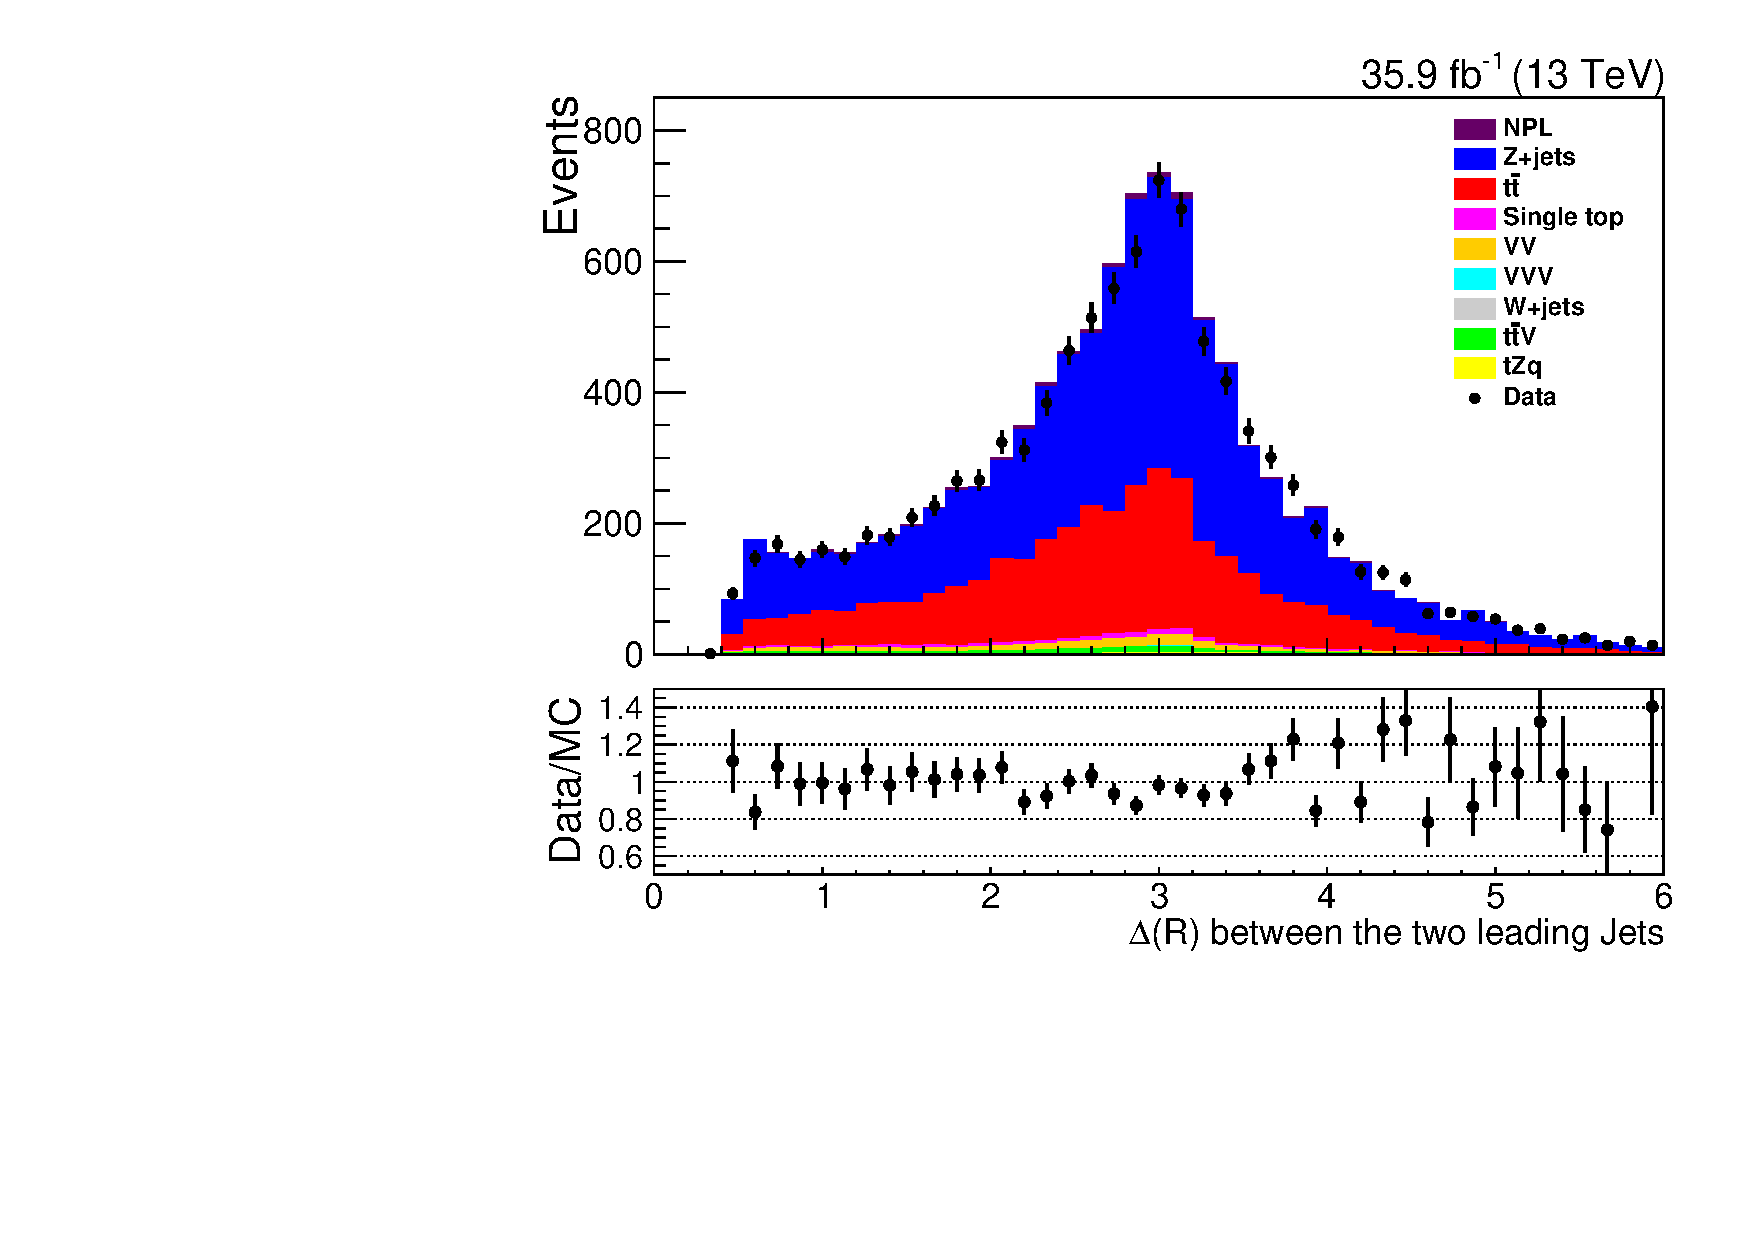
\includegraphics[width=0.47\textwidth]{figs/background-estimation/plots/unblinded/prompt_mumu_ttbarInc/jjDelR_NPL_mumu_wMass_mumu.pdf}
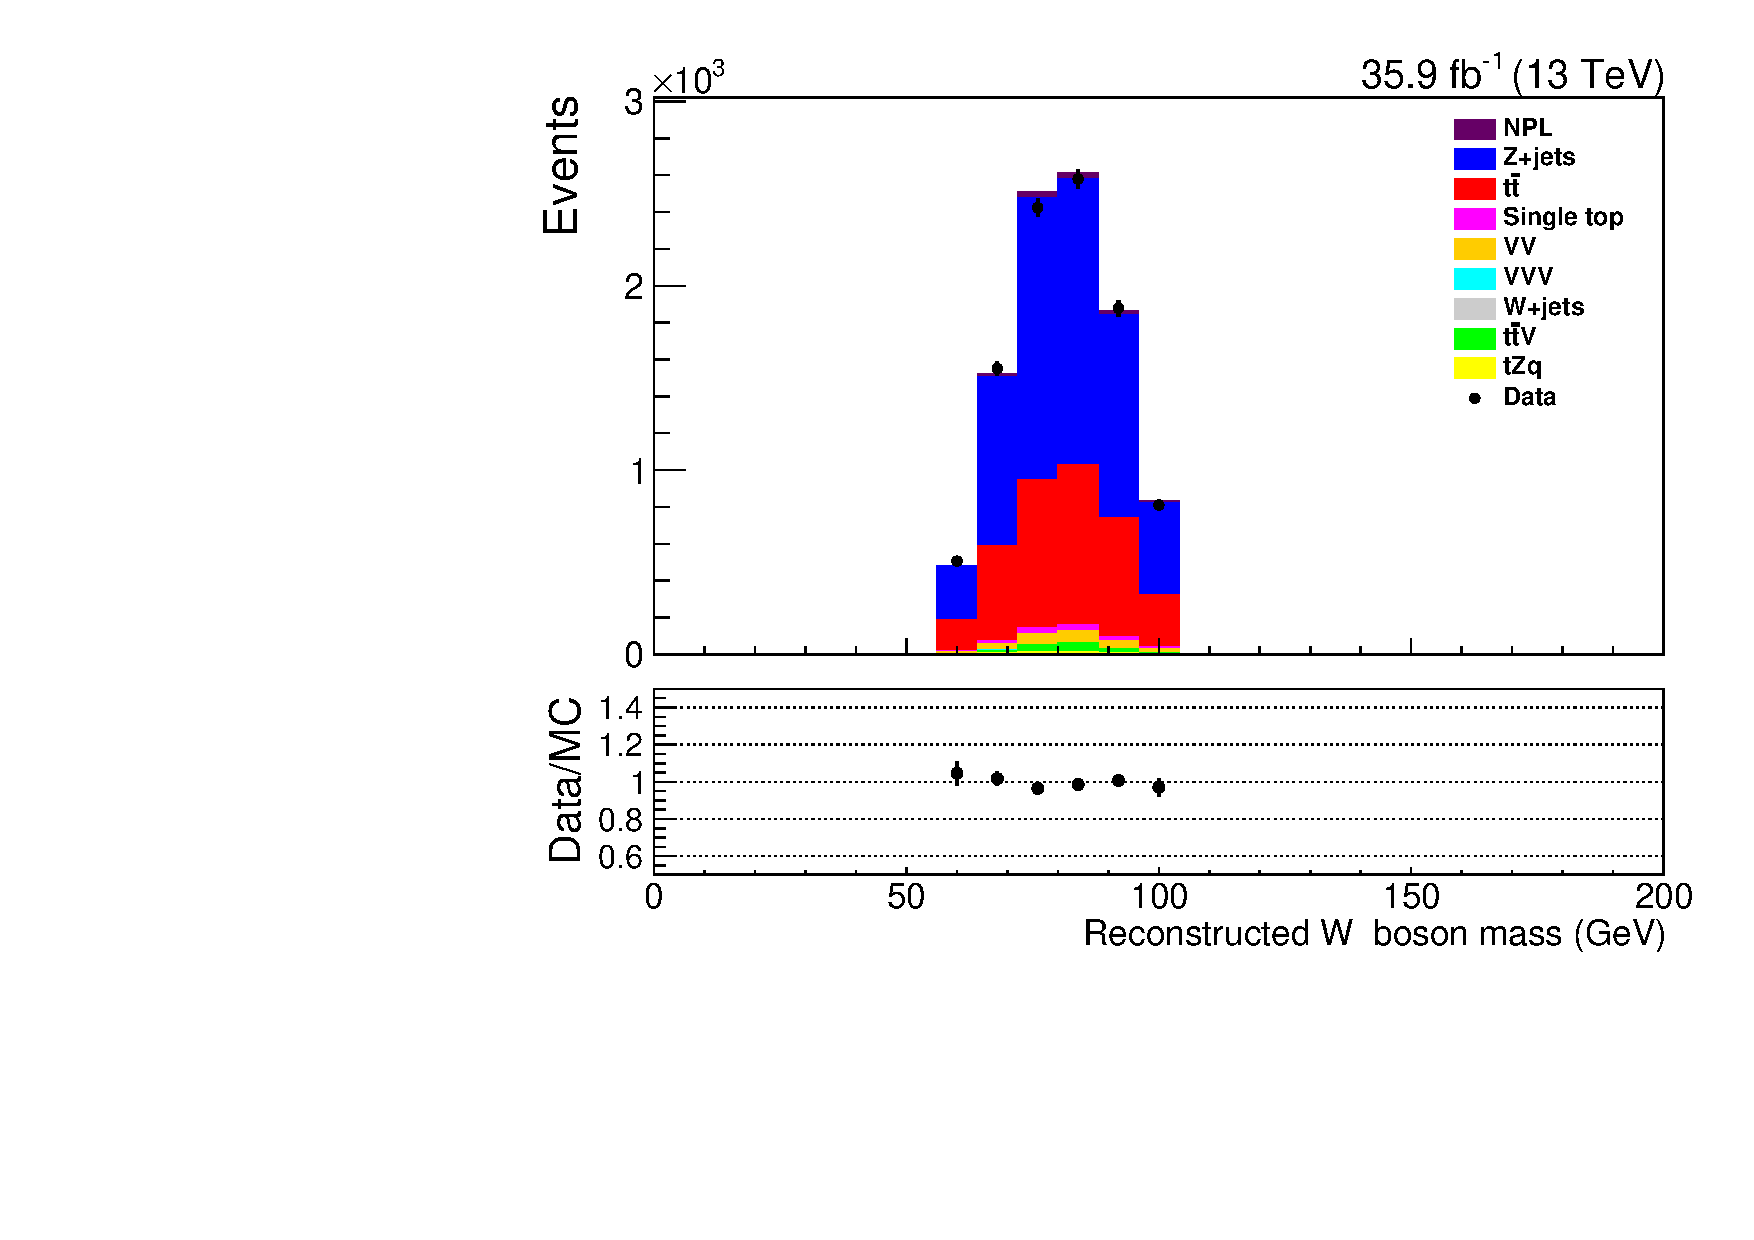
\includegraphics[width=0.47\textwidth]{figs/background-estimation/plots/unblinded/prompt_mumu_ttbarInc/wPairMass_NPL_mumu_wMass_mumu.pdf}
\caption{
Leading b-tagged jet CSVv2 discriminant, leading jet \pT, $\Delta R$ between the leading jets, and reconstructed W boson mass distributions for the $\mu\mu$ channel comparing the agreement between data and simulation for the variables used as input variables in the BDT training.}
\label{fig:inputFeaturesDataSimAgreement11}
\end{figure}

\begin{figure}[htb]
\centering
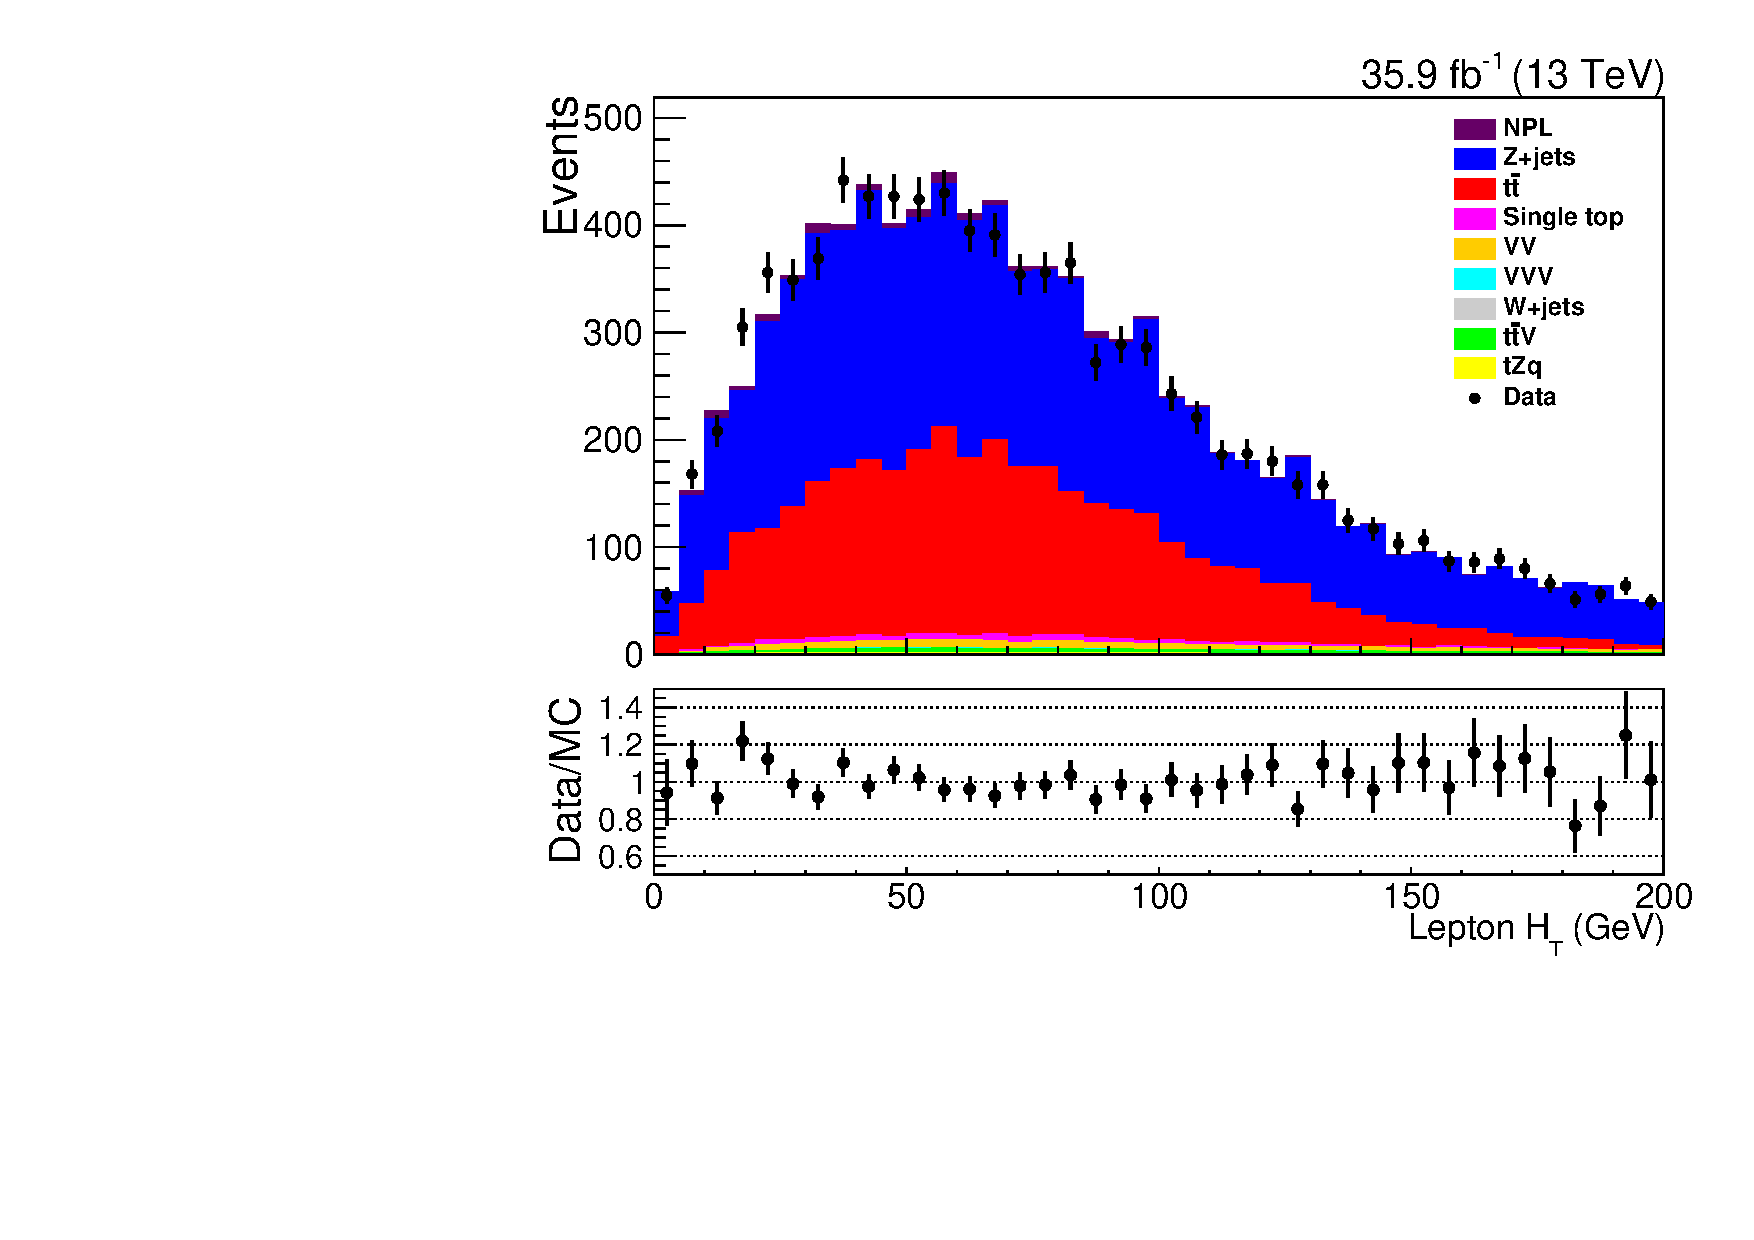
\includegraphics[width=0.47\textwidth]{figs/background-estimation/plots/unblinded/prompt_mumu_ttbarInc/lepHt_NPL_mumu_wMass_mumu.pdf}
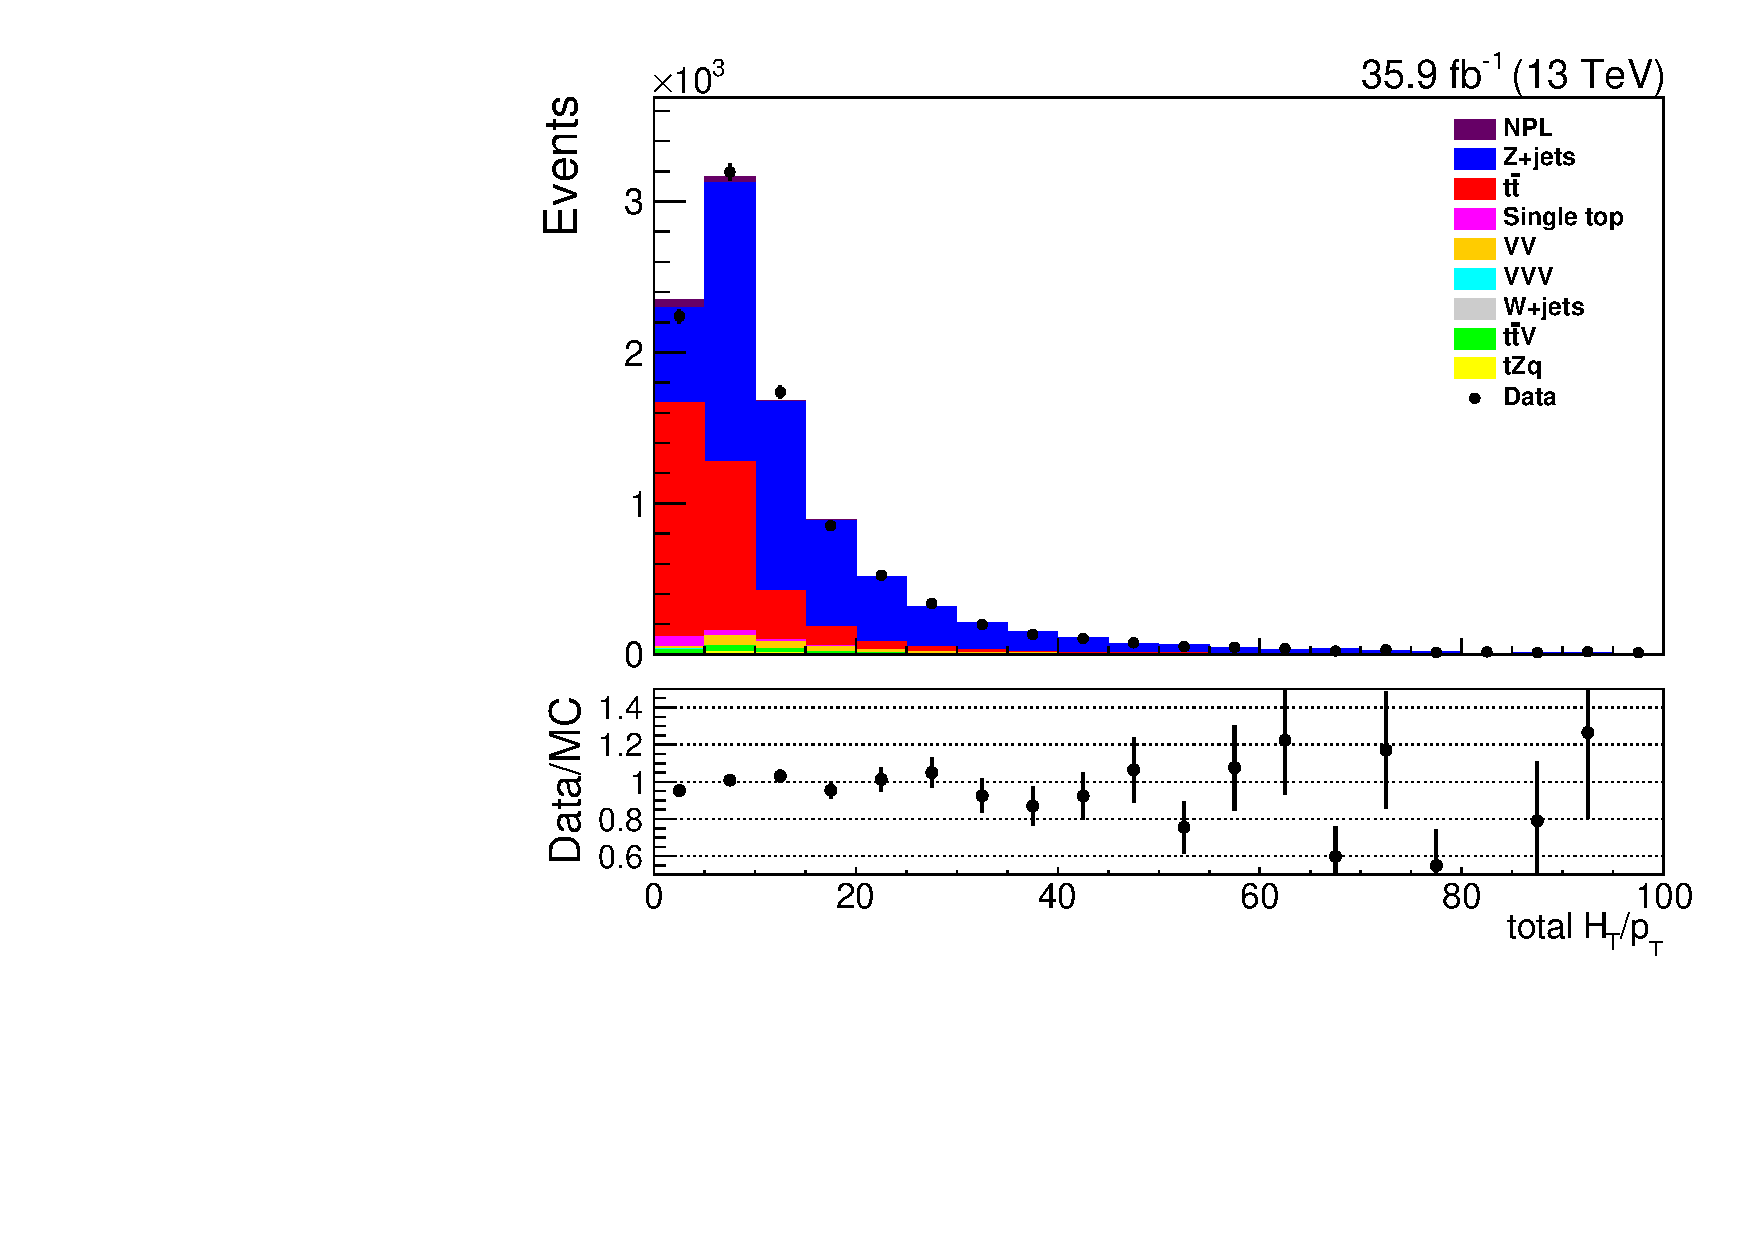
\includegraphics[width=0.47\textwidth]{figs/background-estimation/plots/unblinded/prompt_mumu_ttbarInc/totHtOverPt_NPL_mumu_wMass_mumu.pdf}
\\
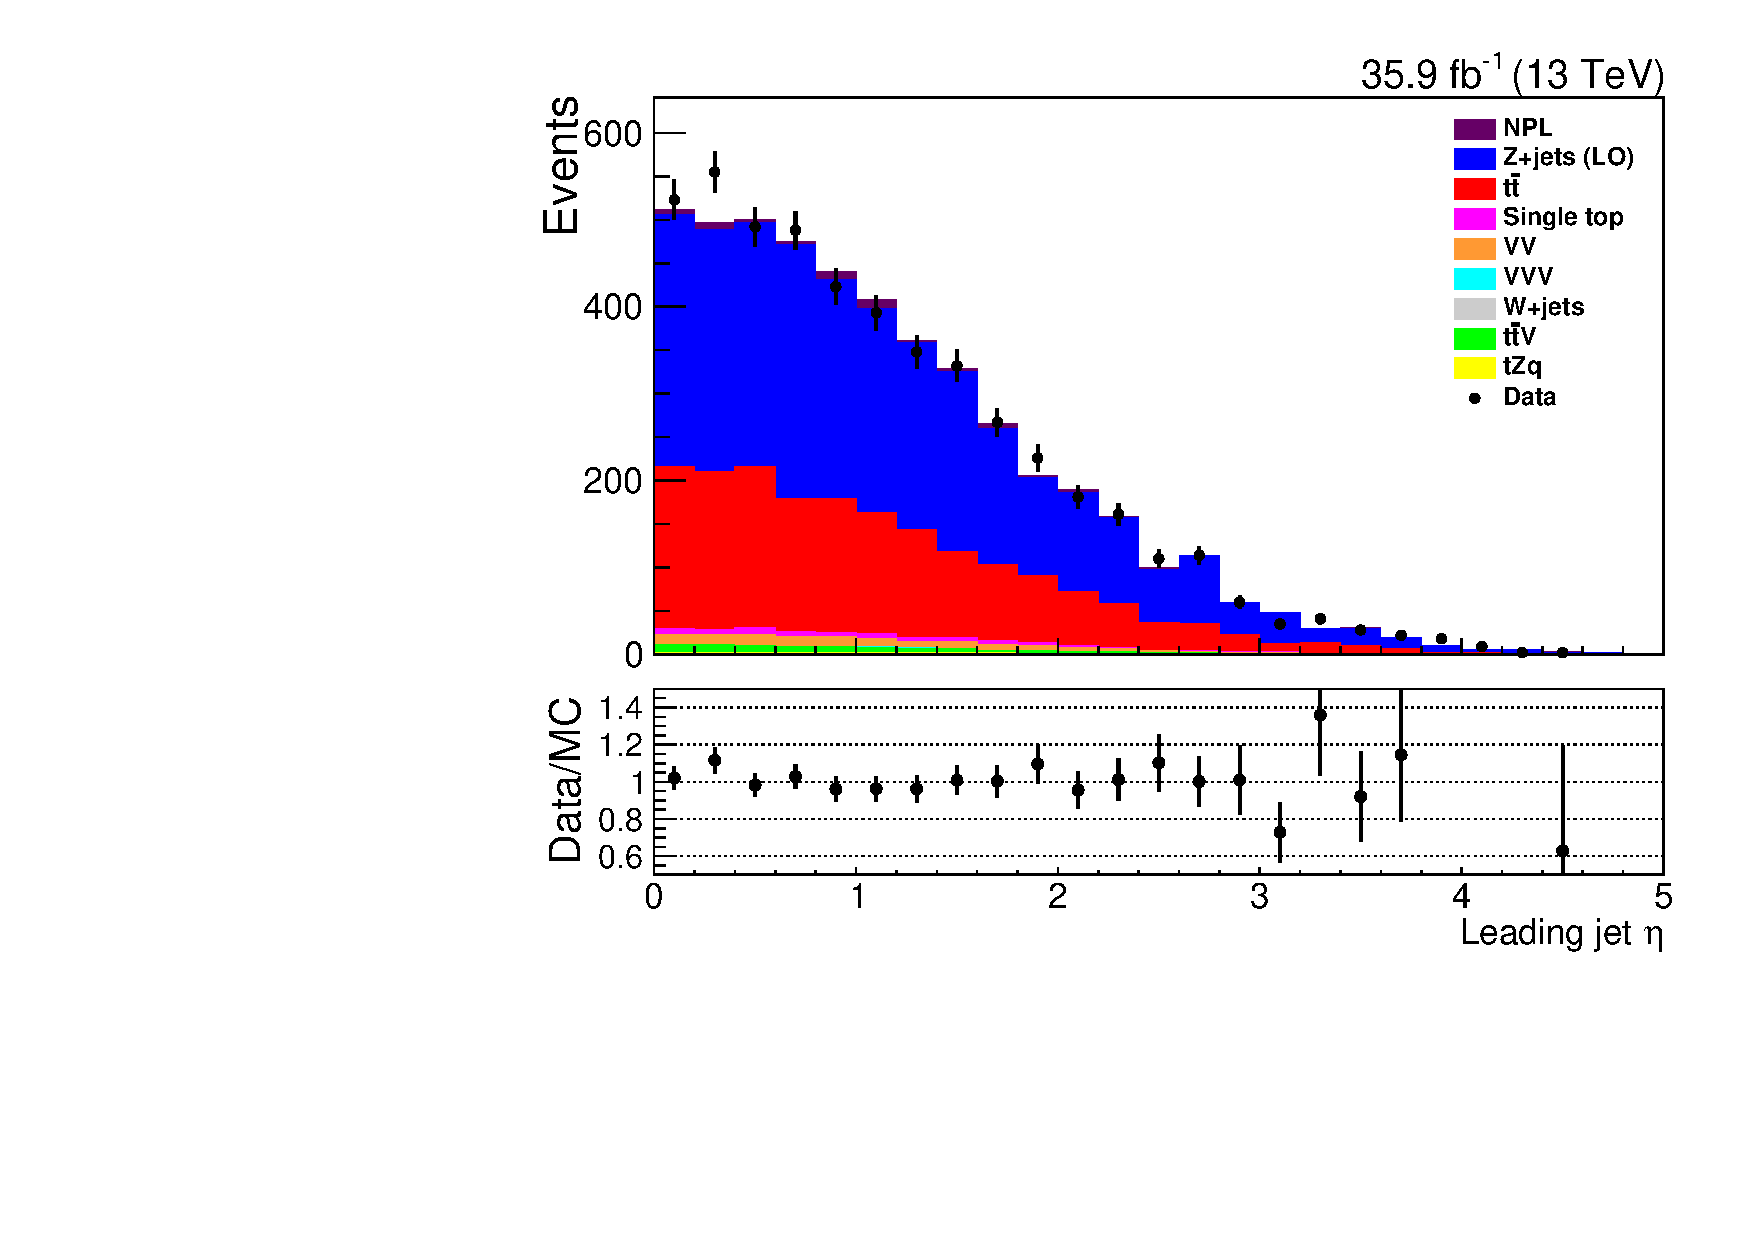
\includegraphics[width=0.47\textwidth]{figs/background-estimation/plots/unblinded/prompt_mumu_ttbarInc/leadingJetEta_NPL_mumu_wMass_mumu.pdf}
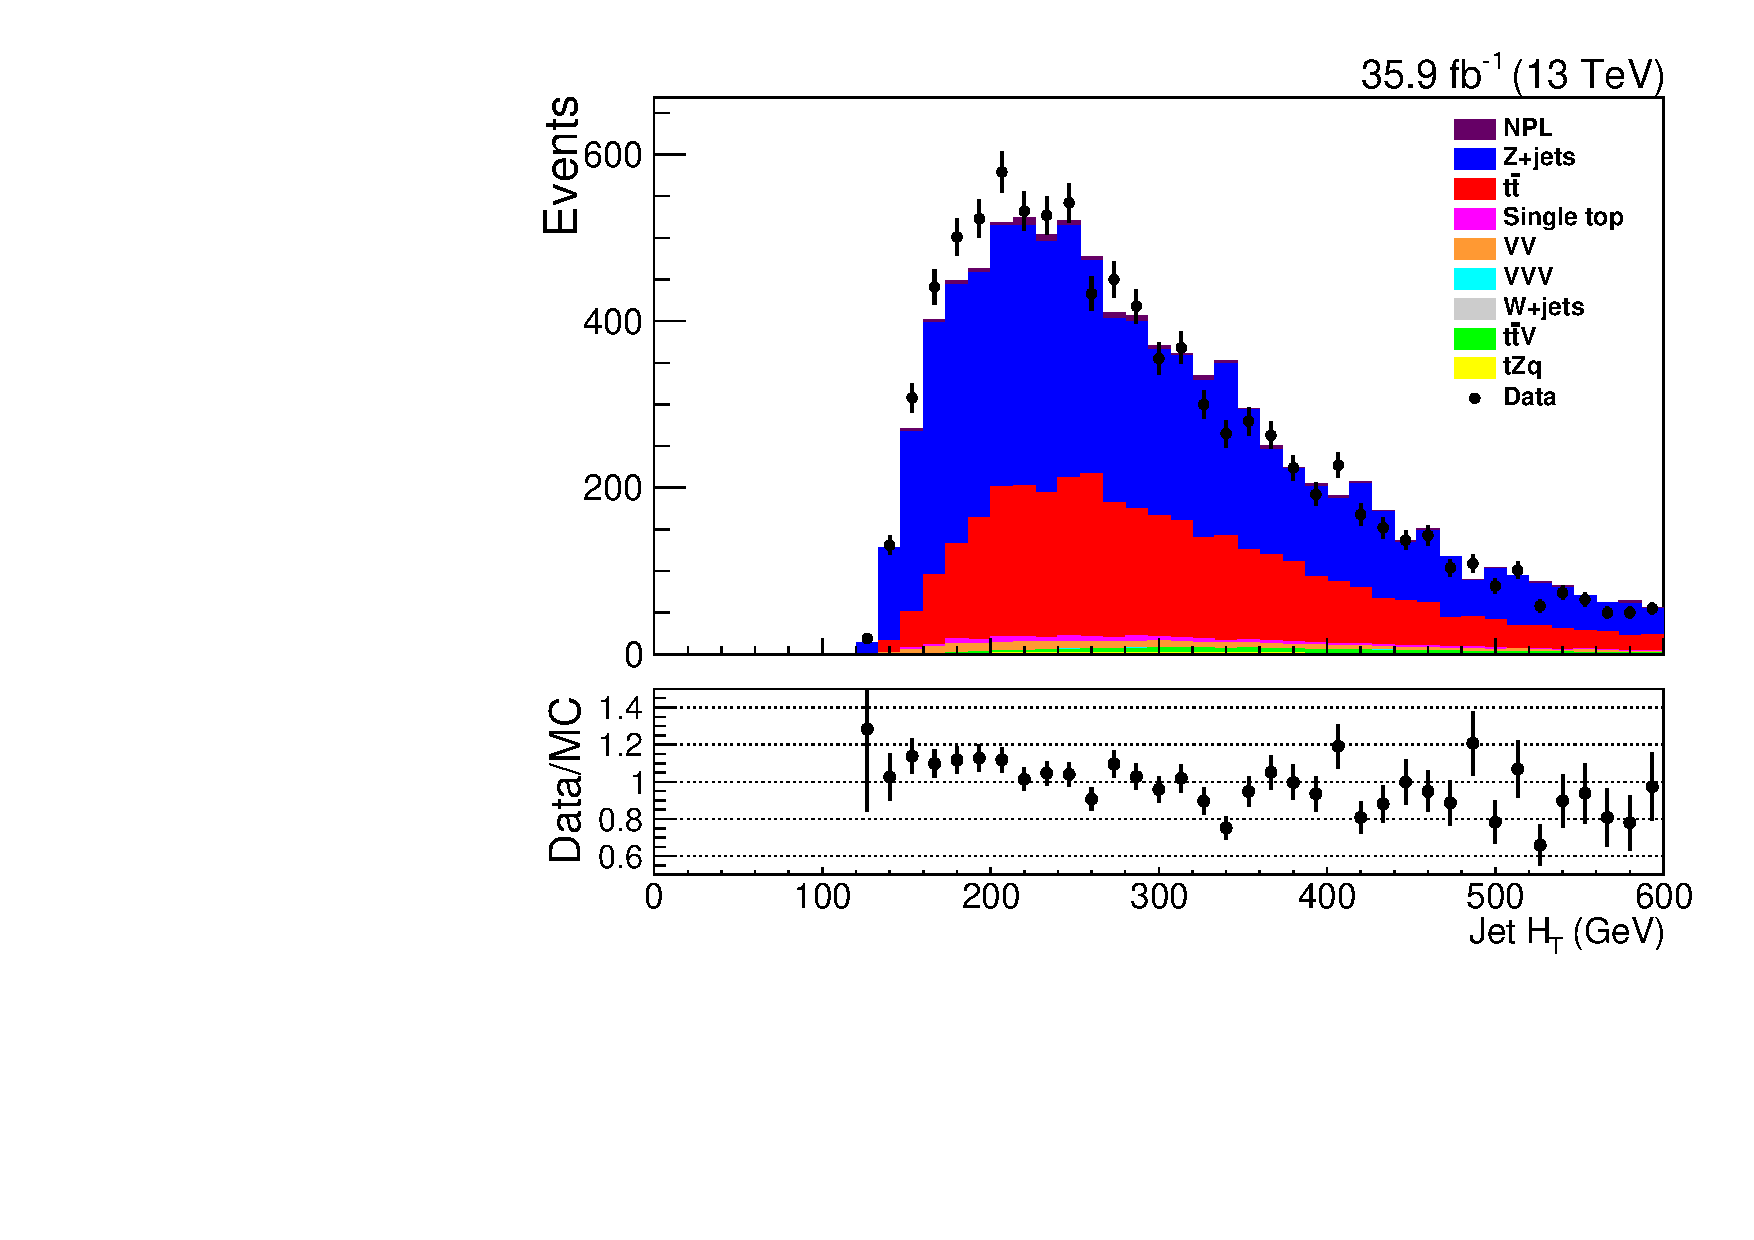
\includegraphics[width=0.47\textwidth]{figs/background-estimation/plots/unblinded/prompt_mumu_ttbarInc/jetHt_NPL_mumu_wMass_mumu.pdf}
\caption{
Lepton ${\ensuremath{H_{\mathrm{T}}}}$, total ${\ensuremath{H_{\mathrm{T}}}}$ divided by total \pt, leading jet $\eta$ and jet ${\ensuremath{H_{\mathrm{T}}}}$ distributions for the $\mu\mu$ channel comparing the agreement between data and simulation for the variables used as input variables in the BDT training.}
\label{fig:appInputFeaturesDataSimAgreement12}
\end{figure}

\begin{figure}[htb]
\centering
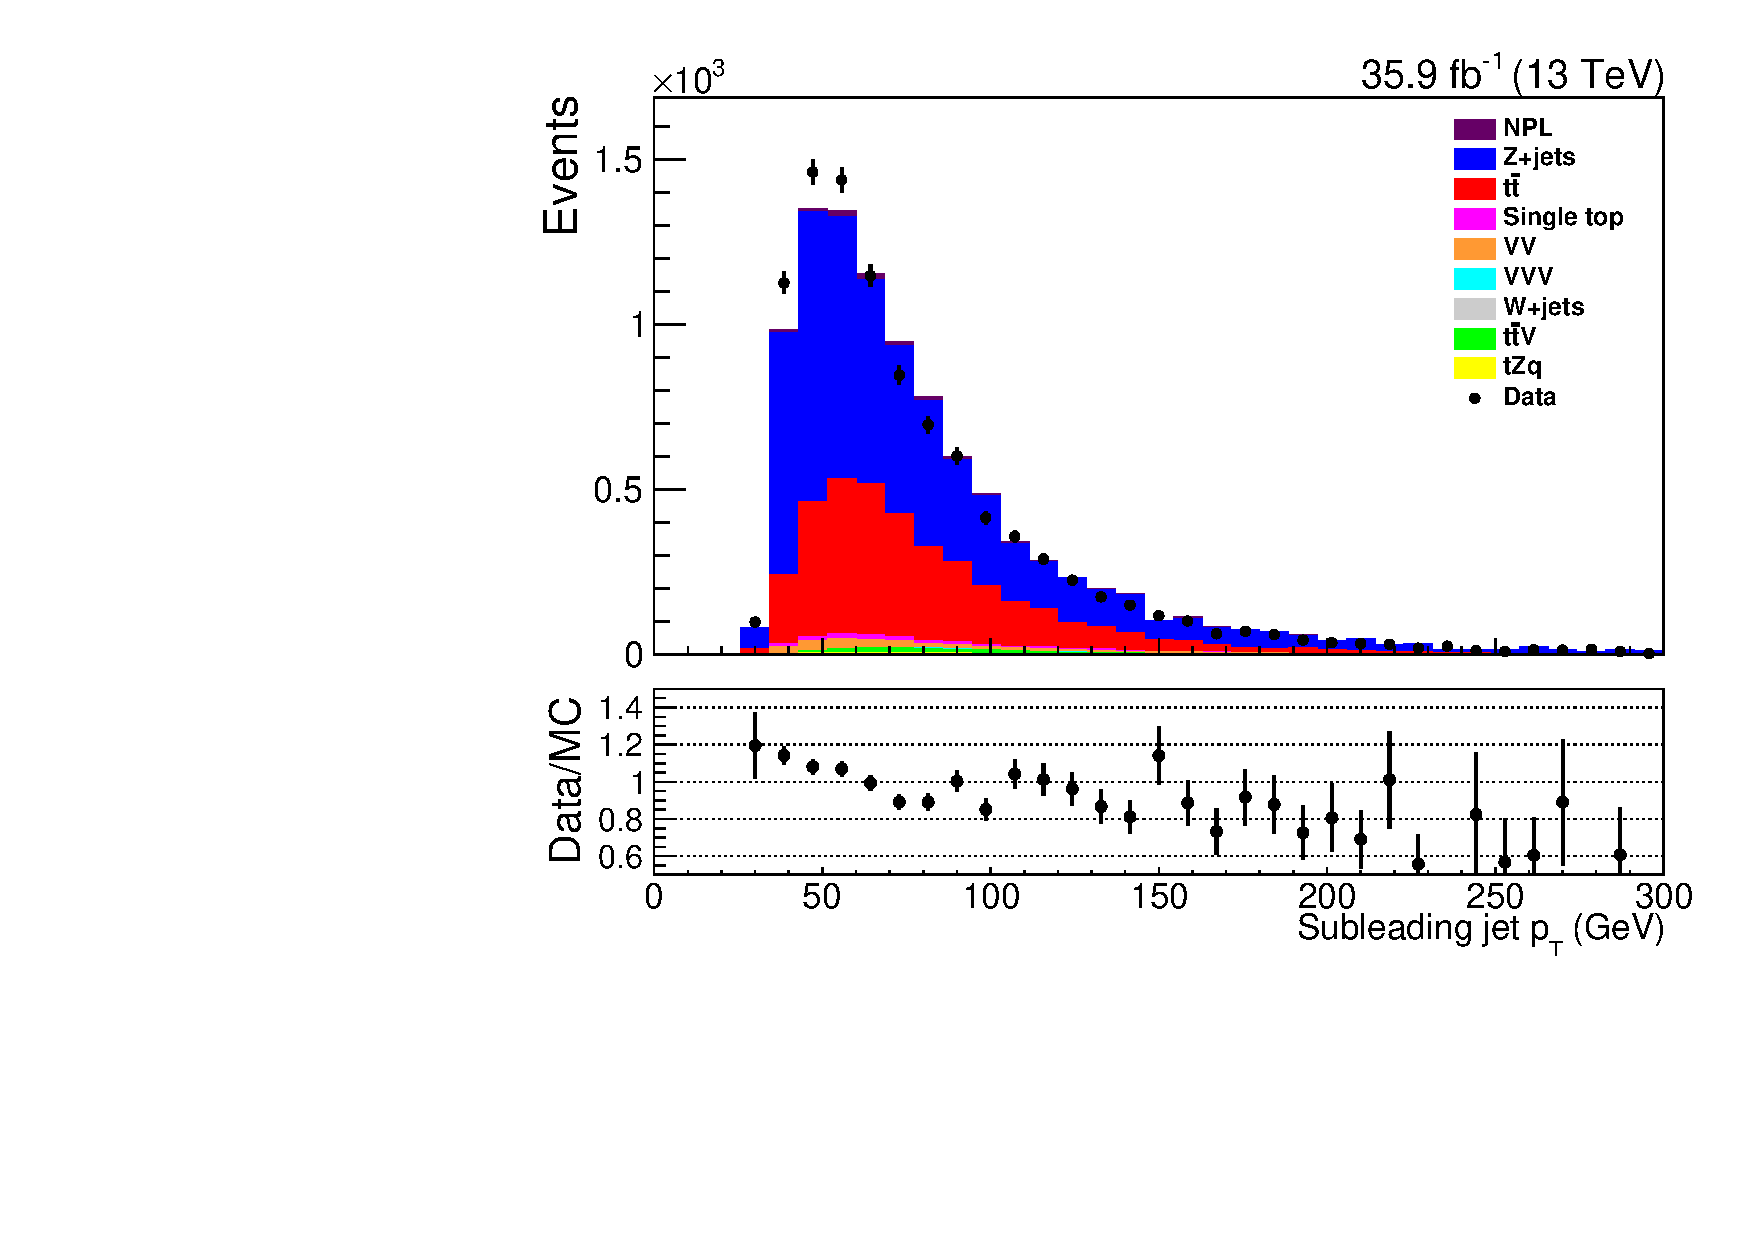
\includegraphics[width=0.47\textwidth]{figs/background-estimation/plots/unblinded/prompt_mumu_ttbarInc/secondJetPt_NPL_mumu_wMass_mumu.pdf}
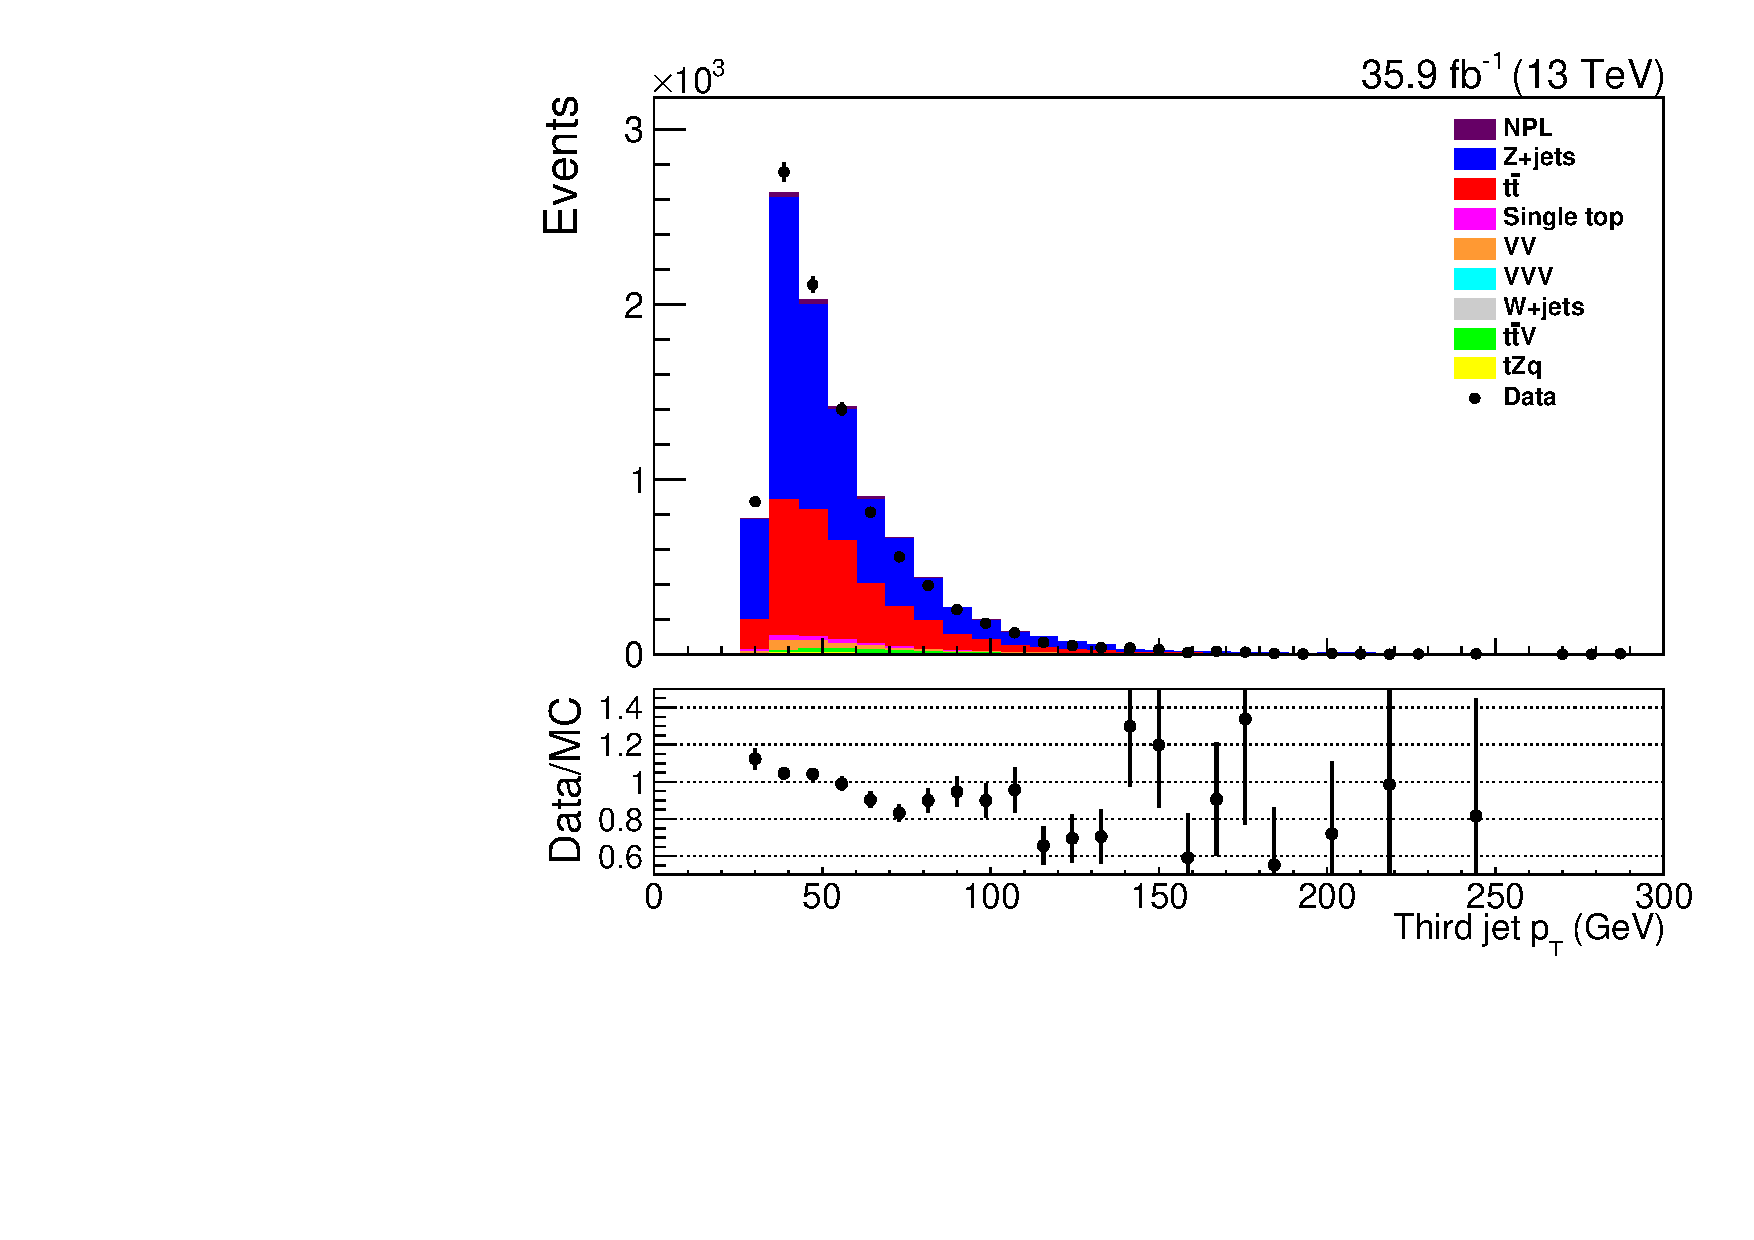
\includegraphics[width=0.47\textwidth]{figs/background-estimation/plots/unblinded/prompt_mumu_ttbarInc/thirdJetPt_NPL_mumu_wMass_mumu.pdf}
\\
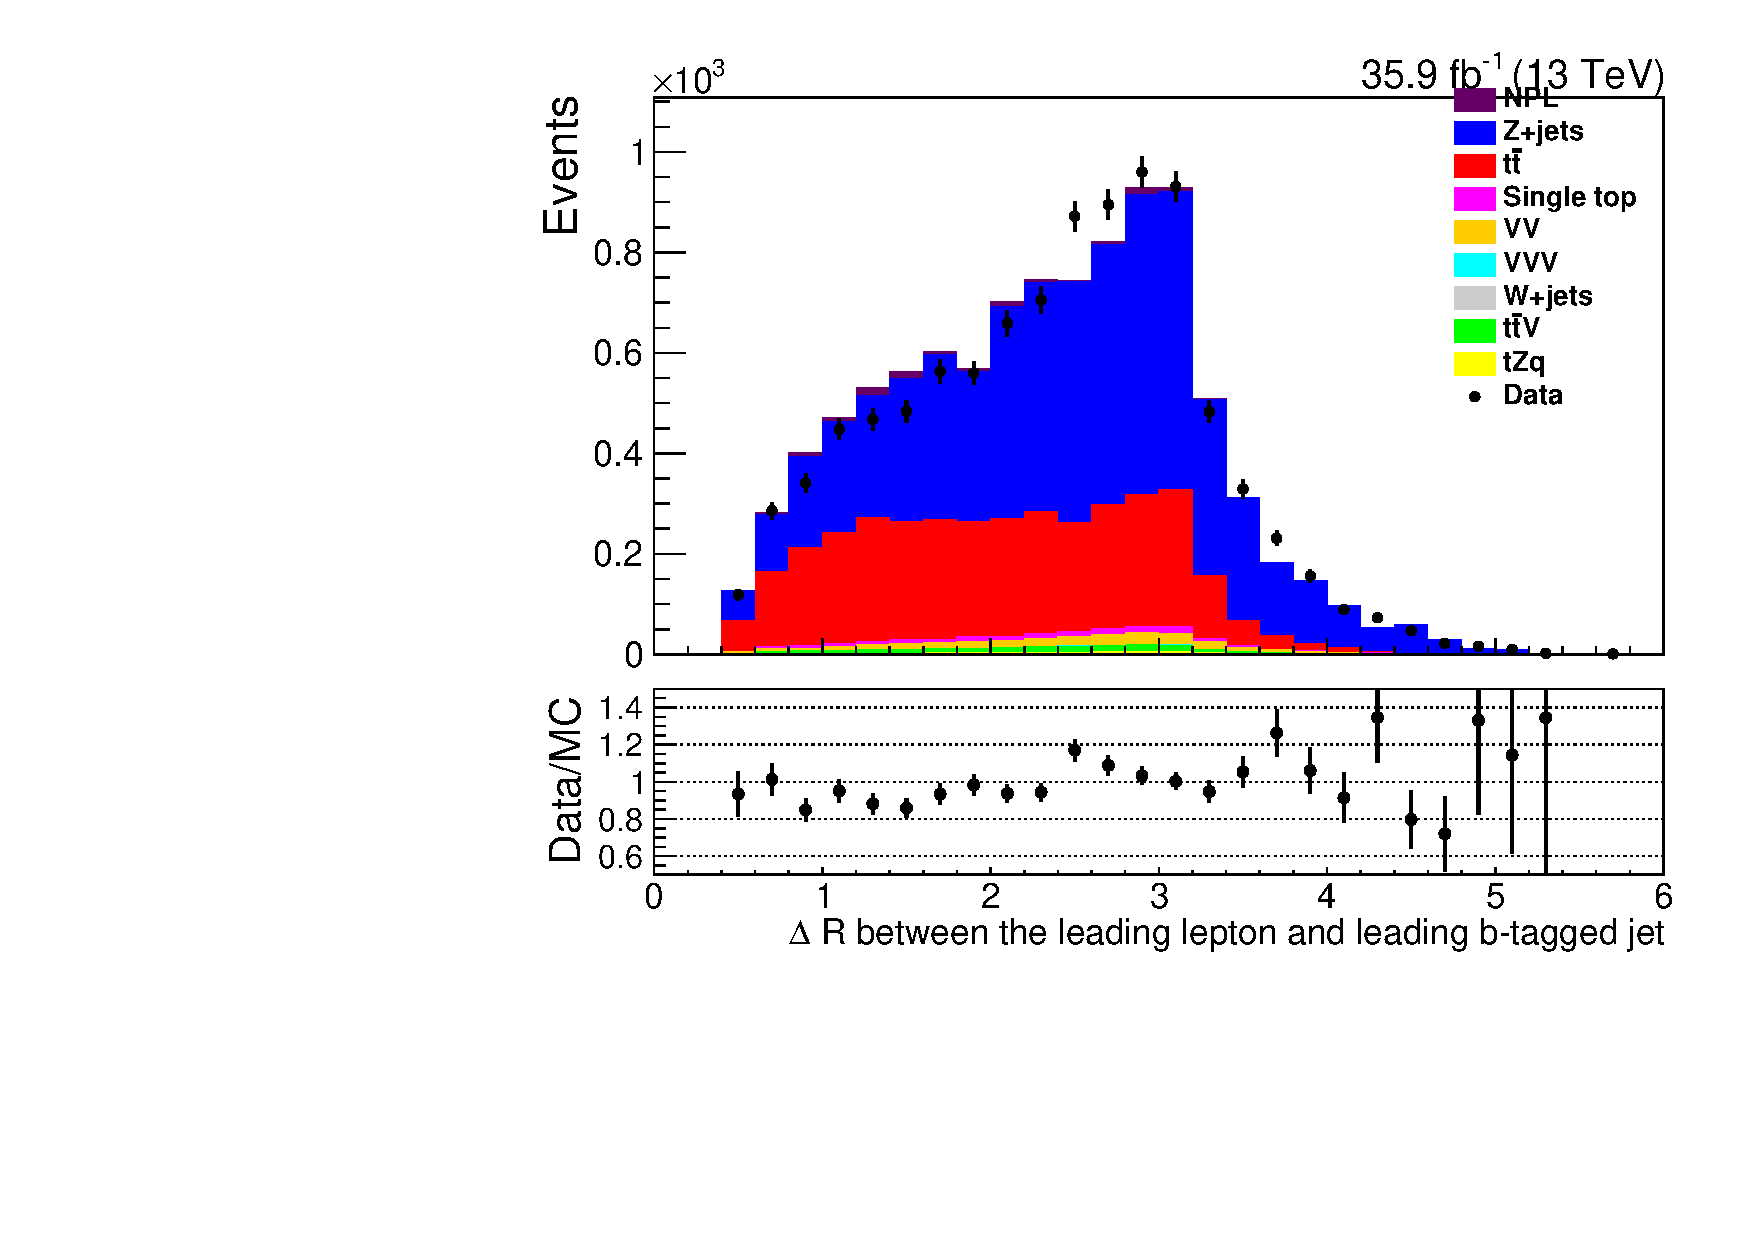
\includegraphics[width=0.47\textwidth]{figs/background-estimation/plots/unblinded/prompt_mumu_ttbarInc/zLep1BjetDelR_NPL_mumu_wMass_mumu.pdf}
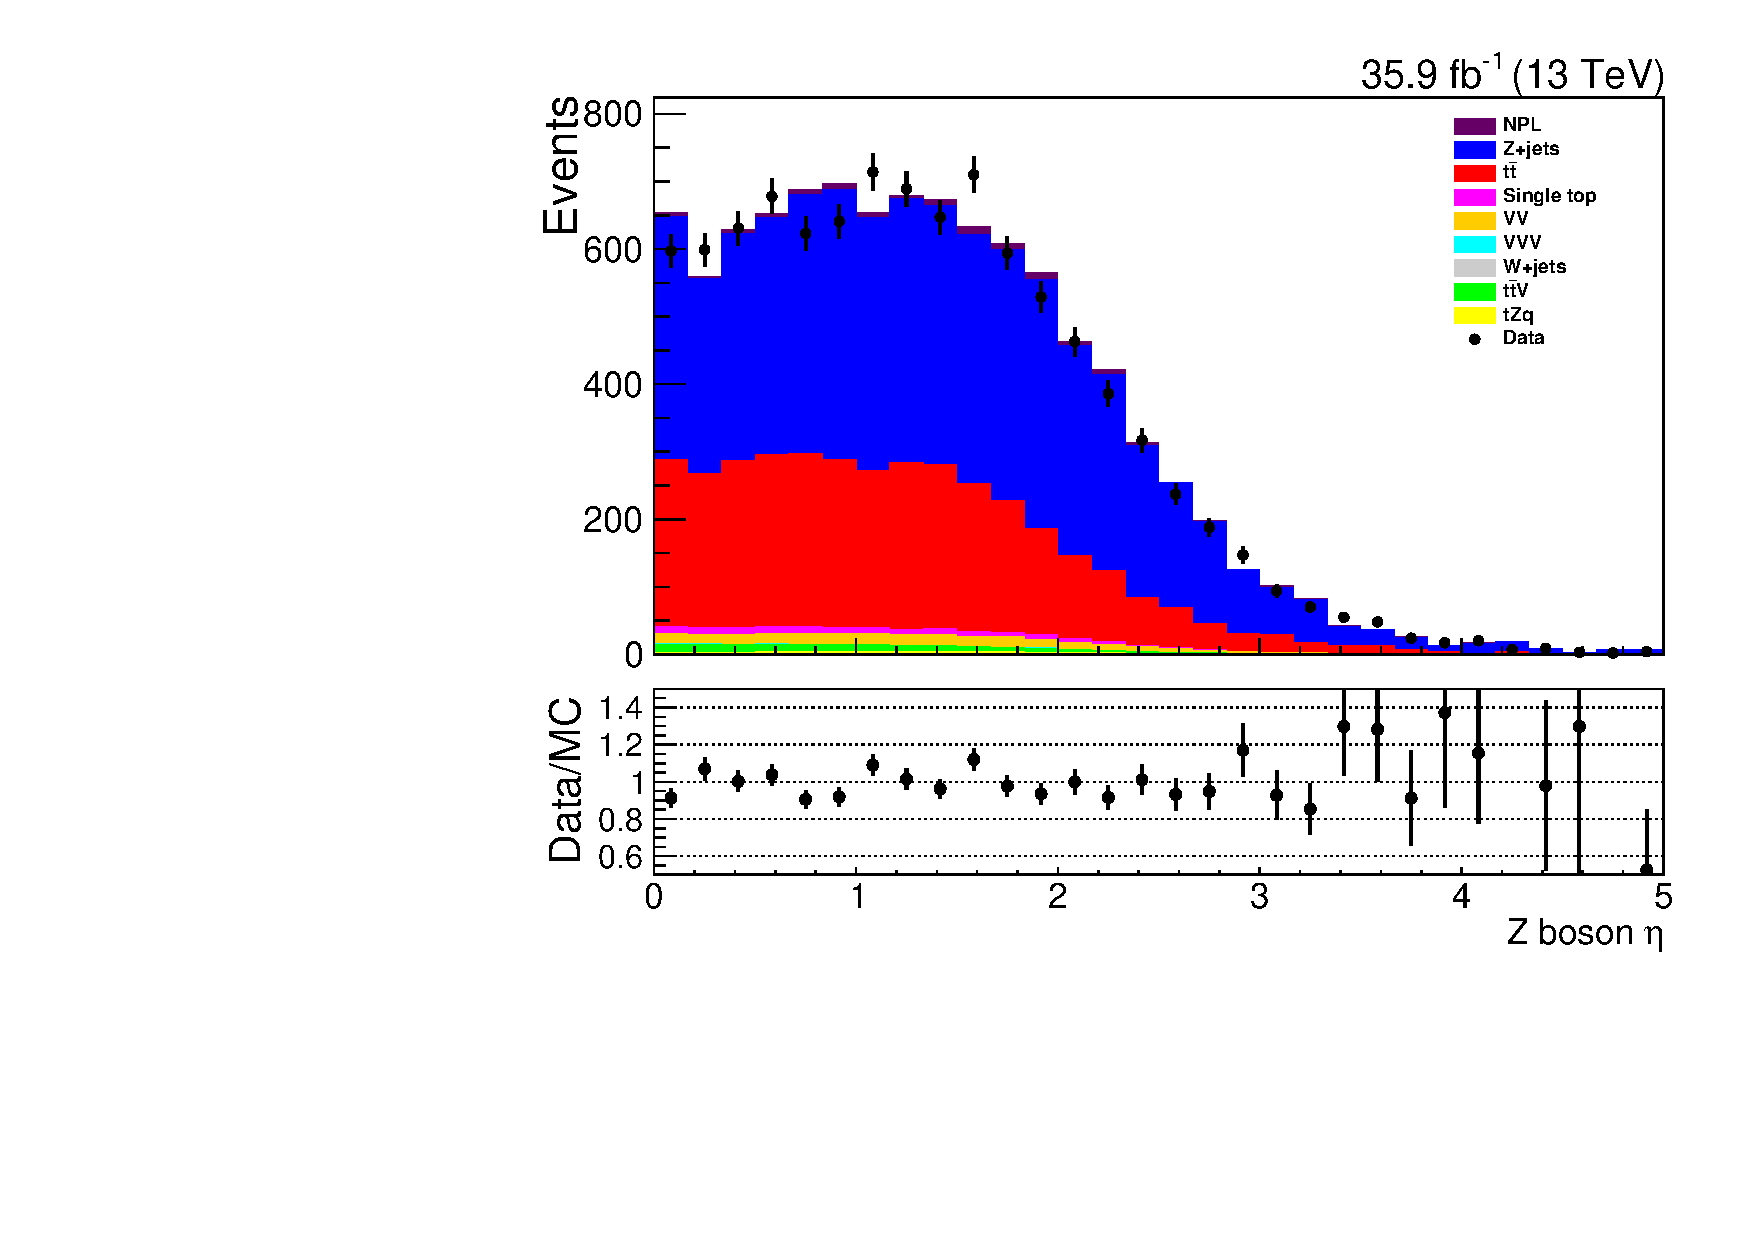
\includegraphics[width=0.47\textwidth]{figs/background-estimation/plots/unblinded/prompt_mumu_ttbarInc/zPairEta_NPL_mumu_wMass_mumu.pdf}
\caption{
Second jet \pt, third jet \pT, $\Delta R$ between leading lepton and leading b-tagged jet and reconstructed Z boson $\eta$ distributions for the $\mu\mu$ channel comparing the agreement between data and simulation for the variables used as input variables in the BDT training.}
\label{fig:inputFeaturesDataSimAgreement13}
\end{figure}
